\documentclass{sig-alternate-10pt}
\usepackage{amsfonts,xspace}
\usepackage{url}
%\usepackage{epsfig}
\usepackage{graphicx}
%\usepackage{subfigure}
\usepackage{ifpdf}
\usepackage{epstopdf}
\usepackage[usenames,dvipsnames]{color}
\newcommand{\ie}{{\it i.e.}\xspace}
\newcommand{\eg}{{\it e.g.}}
\newcommand{\etc}{{\it etc.}}
\newcommand{\useragent}{{\it User-Agent}\xspace}
\newcommand{\httphost}{{\it Host}\xspace}
\newcommand{\httpget}{{\it HTTP GET}\xspace}
\newcommand{\sslservername}{{\it Server-Name}\xspace}
\newcommand{\eat}[1]{}
\usepackage[english,plain]{fancyref}
\usepackage{times}
\usepackage{rotating}
\usepackage[labelformat=simple]{subfig}
\usepackage{multirow}

\newcommand{\mypara}[1]{\medskip\noindent{\bf {#1}:}~}
\newcommand{\chk}{$\checkmark$}
\newcommand{\dsh}{{\bf --}}
\newcommand{\til}{{\bf\large \textasciitilde}}
\newcommand{\tbd}[1]{[{\color{red}{\bf{TBD: #1}}}]}
\newcommand{\drc}[1]{[{\color{blue}{Dave: #1}}]}
%\newcommand{\tbd}[1]{}
\newcommand{\tbdv}[1]{{\color{blue}{!\bf{#1}$_{verify}$}!}}
\newcommand{\etal}{\emph{et~al.}}
\newcommand{\platname}{{\emph{MobiScope}}\xspace}
\newcommand{\platnameT}{{MobiScope}\xspace}
\newcommand{\dsum}{\displaystyle\sum}
\newcounter{packednmbr}
\newcommand{\iphone}{iPhone\xspace}
\newcommand{\wifi}{Wi-Fi\xspace}
\newcommand{\postfigspace}{-1em}
\newcommand{\figcapspace}{0em}
\newcommand{\mobWild}{{\emph{mobWild}}\xspace}

\newenvironment{packedenumerate}{\begin{list}{\thepackednmbr.}{\usecounter{packednmbr}\setlength{\itemsep}{0.2pt}\addtolength{\labelwidth}{-4pt}\setlength{\leftmargin}{\labelwidth}\setlength{\listparindent}{\parindent}\setlength{\parsep}{1pt}\setlength{\topsep}{0pt}}}{\end{list}}
\newenvironment{packeditemize}{\begin{list}{$\bullet$}{\setlength{\itemsep}{0.2pt}\addtolength{\labelwidth}{-4pt}\setlength{\leftmargin}{\labelwidth}\setlength{\listparindent}{\parindent}\setlength{\parsep}{1pt}\setlength{\topsep}{0pt}}}{\end{list}}
\newenvironment{packedtrivlist}{\begin{list}{\setlength{\itemsep}{0.2pt}\addtolength{\labelwidth}{-4pt}\setlength{\leftmargin}{\labelwidth}\setlength{\listparindent}{\parindent}\setlength{\parsep}{1pt}\setlength{\topsep}{0pt}}}{\end{list}}

%\renewcommand{\fref}{\S\ref}
\renewcommand\thesubfigure{~(\alph{subfigure})}

\title{MobiScope: Pervasive Internet Traffic Monitoring for Mobile Devices}

\numberofauthors{7}
\author{
\alignauthor
Ashwin Rao\\
\affaddr{INRIA}
\alignauthor
Amy Tang\\
\affaddr{UC Berkeley}
\alignauthor        
Shen Wang\\
\affaddr{University of Washington}
\and
\alignauthor
Nick Martindell\\
\affaddr{University of Washington}
\alignauthor
Justine Sherry\\
\affaddr{UC Berkeley}
\alignauthor
Walid Dabbous\\
\affaddr{INRIA}
\and
\alignauthor
Arvind Krishnamurthy\\
\affaddr{University of Washington}
\alignauthor 
Arnaud Legout\\
\affaddr{INRIA}
\alignauthor
David Choffnes\\
\affaddr{Northeastern University}
}
% Remove additional authors section
\def\addauthorsection{}
\date{}
\begin{document}	
\maketitle

\subsection*{Abstract}

We present, Meddle, a platform that relies on traffic indirection to diagnose mobile Internet traffic.
Meddle is motivated by the absence of built-in support from ISPs and mobile OSes to freely monitor and control mobile Internet traffic; the restrictions imposed by mobile OSes and ISPs also make existing approaches impractical.
%Instrumenting mobile OSes, static and dynamic analysis of application binaries, or the privilege of working with ISPs---impractical. 
Meddle overcomes these hurdles by relying on the native support for traffic indirection by mobile OSes.
Specifically, Meddle proxies mobile Internet traffic through a software defined middleboxes configured for mobile traffic diagnosis. 
In this paper, we use Meddle to tests the limits of the network perspective of mobile Internet traffic offered by traffic indirection. 

We use this perspective to characterize and control the behavior of mobile applications and provide a first look at ISP interference on mobile Internet traffic. 
\tbd{We report on controlled experiments we conducted to analyze the network behavior of 100 most popular iOS and Android applications.}
\tbd{We also report on how ISP interfere with mobile HTTP Internet traffic.}








%%% Local Variables: 
%%% mode: latex
%%% TeX-master: "meddle-main"
%%% End: 


\section{Introduction}
\label{sec:introduction}

%what is the problem area you are working in and why is it important? It is important to set the larger context here. Why is the problem of interest and importance to the larger community?

Mobile systems consist of walled gardens inside gated communities, i.e., locked-down operating systems running on devices that interact over a closed and opaque mobile network. 
Despite a large collection of privacy, policy and performance issues in mobile networks~\cite{enck:taintdroid,hornyack:appfence,speedtest,pathak:eprof}, researchers are faced with few options to characterize and address them.

%What is the specific problem considered in this paper? This paragraph narrows down the topic area of the paper. In the first paragraph you have established general context and importance. Here you establish specific context and background.
%Cannot mention user participation and crowd sourcing here because we have not achieved it in this work . 
%What we have here is a platform with a potential for user participation and preliminary results. 

The key challenge is that mobile devices, their OSes, and ISPs provide no built-in service to monitor and control \emph{all network traffic}.
As a result, previous studies~\cite{vallina-rod:ads,gerber:passivespeed,chen:wifi,enck:taintdroid,wang:middleboxes,sommers:cellwifi} are constrained by at least one of the following: mobile OSes, access technology, device manufacturer, installed applications, and user behavior.
In this work, we are the first to present an approach that compromises none of these, an approach that can be used across carriers, mobile devices, apps, and access technologies.

\meddle redirects all Internet traffic through a software-defined middlebox for the purpose of analysis and interposition.
Specifically, \meddle builds on the native support for VPN tunnels by mobile OSes to tunnel all the Internet traffic regardless of the access technology used by the device. 

\tbd{tripwire stuff}


In this paper, we use \meddle to test the limits to which mobile Internet traffic can be diagnosed using traffic redirection.
The main contributions of this paper are as follows:
\begin{packedenumerate}
\item Platform for practical mobile diagnosis. Single server solution empowers users to install and configure them on home-gateways.
Researchers can deploy them for measurement studies. 
\item Controlled experiments using off-the-shelf Android and iOS devices. 
\item Controlled experiments to analyze ISP interference in US and France. 
\end{packedenumerate}

The remainder of this paper is structured as follows.

%%% Local Variables: 
%%% mode: latex
%%% TeX-master: "meddle-main"
%%% End: 



\section{MobiScope Overview}
\label{sec:platform}

% This section describes the goals for our monitoring approach, and how
% \platname achieves these goals using proxying.  We show that our
% approach imposes reasonable overheads, and we describe how our
% IRB-approved study protects user privacy.

% \subsection{Goals}
% \label{sec:goals}
% Our primary goal is \emph{to monitor all the Internet traffic from
%   mobile devices regardless of the operating system, wireless access
%   technology, and the ISPs used by the mobile device}.  To achieve
% this goal, we identify the following desirable properties for a
% measurement platform:
% \begin{packedenumerate}
% \item \emph{Portable.} Our approach should work on all major device
%   OSes without requiring support from carriers or ISPs.
% \item \emph{Pervasive.} We should be able to measure traffic
%   regardless of the location, access technology, and ISPs used by
%   mobile devices.
% \item \emph{Passive.} We wish to understand the network traffic
%   naturally generated by users and their devices, requiring passive
%   monitoring.
% \item \emph{Deployable.} We want a low barrier to entry to facilitate
%   large-scale adoption with minimal impact on the user
%   experience. \tbd{We need to say easy to controlled perform
%     experiments}
% \end{packedenumerate}

In this section, we present an overview of the \platname{} platform\footnote{Our platform is currently in private beta with deployments in the US, France and China. We will make the \platname{} software publicly available.}. The goal of \platname{} is straightforward: we 
 seek to enable passive monitoring of \emph{all
  the Internet traffic from and to mobile devices}. While previous work has accomplished 
  this for a limited set of devices or networks, we seek to avoid such limitations. 
\begin{packedenumerate}
\item \emph{OS agnostic.} Monitor traffic independently of
  the OS run by the monitored device. In particular, we avoid the need to 
  develop OS-specific applications, or to root or jailbreak the device.
\item \emph{ISP agnostic.} Monitor traffic without any
  support from ISPs and cellular providers.
\item \emph{Access technology agnostic.} Monitor traffic
  whatever the access technology used by the mobile device (Wifi, GSM,
  CDMA, UMTS, LTE, etc.)
\item \emph{Continuous.} Monitor traffic continuously, even when devices switch 
between networks or return from being idle.

\tbd{There is not more reference to the flow modification (admittedly
  a bad term) feature. Don't we want to put it as a design
  goal. Section "Interposing on Traffic on Mobiscope" is just about
  that. May be we can add the goal "Traffic interposition".}
%\item \emph{Flow modification.} We want to not only monitor, but
 % also possibly modify data packets in order to experiment. This makes
 % \platname{} both a passive monitoring and an experimental
 % platform. 
\item \emph{Scalability.} \platname{} should be equally feasible to deploy 
on a single machine or using a collection of VMs in a hosted/cloud deployment. 

\item \emph{Encryption agnostic.} Achieve visibility of both encrypted and plaintext traffic.

 \end{packedenumerate}    
 

In the following, we describe in detail the design of \platname{},
then we discuss the limitations of the platform.


\subsection{MobiScope Design}

% We now describe how we achieve these goals using proxying.
% Specifically, we use two approaches to proxy mobile traffic: secure
% proxying via virtual private networks (VPNs) and insecure transparent
% proxying.  These two approaches allow us to measure traffic with and
% without carrier interposition, respectively.

% \subsubsection{VPN Proxying}
% \label{sec:platform-vpn}

To meet the above goals, we exploit the observation that nearly all 
devices support network traffic indirection via virtual private networks (VPNs). 
In particular, instead of using the VPN server to access a private network, 
we use it as a proxy for all of a device's mobile Internet traffic. This enables passive monitoring 
of Internet traffic regardless of device OS, carrier/ISP or access technology. 
Further, we show that this approach has minimal impact on 
performance and measurement fidelity -- making \platname{} a practical 
approach for pervasive passive network monitoring.

In the following sections, we describe how our measurement infrastructure 
achieves the goals stated in the previous section. We begin by describing 
how we addressed several challenges with implementing our VPN-based 
proxy. 


% designed the \platname{} platform
%on a VPN infrastructure. By instrumenting the VPN server that
%mobile devices are using, we can monitor all the Internet traffic going
%through the VPN tunnels. But, using a VPN infrastructure raises three
%important questions. i) How ubiquitous is the VPN technology on mobile
%devices?  ii) How to monitor traffic on \platname{}? iii) How to
%modify traffic on \platname? We explore in the following these three key questions.

\subsubsection{VPNs for Mobile Devices}
\label{sec:vpn-tech-mobile-device}
In this section, we provide a detailed description of how VPNs allow 
us to achieve many of our \platname{} design goals.  
Our first goal is to provide a measurement system that works regardless 
of device OS. To achieve this goal, we note that VPNs are widely supported 
on the most popular mobile OSes. Indeed, Android, BlackBerry, Bada, and iOS all support VPNs,
primarily to satisfy their enterprise clients. In this work, we focus on 
the two most popular OSes: iOS and Android. 

Our second and third goals are 
to enable measurements regardless of ISP or access technology. 
Fortunately, iOS and Android support VPN connectivity regardless of  
ISP or access technology -- so long as the network supports the Internet Protocol. 

We note that both iOS and Android support VPN connections 
using the IPSec standard, meaning we can implement our VPN proxy 
server using robust, open-source code from Strongswan~\cite{strongswan}. 
\platname{} thus supports IPSec tunnels using either IKEv1 or
IKEv2~\cite{rfc5996} for authentication and key negotiation.


To meet our goal of continuous network monitoring,
a VPN must always be enabled. Currently, all iOS devices (version 3.0
and above) support a feature called \textit{VPN On-Demand}.  VPN
On-Demand forces the iOS device to use VPN tunnels when connecting to
a specified set of domains. To ensure all possible addresses match this list, 
we observed that iOS uses suffix matching to determine which connections 
should be tunneled; accordingly, we specified the domain list as the set of 
alphanumeric characters (a-z, 0-9, one character per domain). 
Android version 4.2 and above support an
\textit{Always On VPN} connection that is always enabled for all data
traffic, and Android version 4.0 and above provide an API that allows
applications to manage VPN tunnels. We support both options: we have distributed Always On VPN 
configurations and implemented an application that
uses the VPN API to provide equivalent functionality for
Android 4.0 and 4.1.


% The use IPsec by mobile devices for pervasive VPN tunnels limited our
% choice of VPN daemons to manage VPN tunnels on our proxying server.
% Though VPN daemons manage tunnels created using protocols such as PPTP
% and L2TP, the ``VPN On-Demand'' feature of iOS is available only for
% VPN tunnels that use IPsec.  To the best of our knowledge, the only
% publicly available VPN daemon that uses IPsec in Linux \emph{without
%   any kernel modifications} is Strongswan~\cite{strongswan}.
% Strongswan also supports the faster IKEv2~\cite{rfc5996} based
% authentication which is supported by Android devices.

% \subsubsection{Advantages and Drawbacks of VPNs}
% \label{sec:advant-drawback-vpn}



\subsubsection{Monitoring Traffic on MobiScope}
\label{sec:monit-traff-mobiscope}



Having shown that VPNs support many of \platname{}'s goals, 
we now describe how we implement passive network monitoring 
using VPN proxying. While the high-level design for capturing 
network traffic from mobile devices is straightforward, the implementation 
is not. In particular, the interactions between IPSec, routing and NAT 
complicate our ability to map bidirectional flows to individual devices. 
The following paragraphs describe these challenges and how we 
addressed them to provide a stand-alone (\ie, single server) mobile-traffic monitoring 
proxy. We conclude by describing how our architecture facilitates 
pluggable modules for performing custom monitoring.

At first glance, capturing all traffic traversing a VPN server should be 
as simple as running a tap on the network interface, \eg using \textit{tcpdump}. 
While this indeed captures all traffic, it does not capture sufficient information 
to distinguish bidirectional flows and map them to individual devices. We now 
describe how to provide this mapping.

First, we describe how the Linux network stack interacts with IPSec. 
We assume the \platname{} server is assigned 
IP address $m$ and the mobile device's public IP address is $d$. When 
the VPN connection is established, the proxy assigns the device a private address 
$v$. Last, the device is attempting to access a service located at address $w$. 
We denote a packet from source $s$ to destination $d$ as $s \rightarrow d$.

\noindent \textbf{Forward path.} The first step is to map flows in the forward direction. Figure~\ref{fig:packet-monitor-a} shows the path that packets take 
through a \platname{} proxy.  At steps (1),
(2), and (3) the encrypted datagram (in gray, $d \rightarrow m$) is passed to the IPSec 
module to decrypt and process the encapsulated IP datagram ($v \rightarrow w$) sent from 
the device. Because the \platname{} assigns private address space to 
clients, it must use NAT in step (5) to convert the private IP address \emph{v} to the public IP
address \emph{m}. Last, the packet is forwarded to the Internet. 

We now describe how running tcpdump and tracking the VPN assignment
table\footnote{\platname{} maps a device identified by its public IP
  address to a private IP address in the VPN. We call the mapping
  between this device public and private IP addresses the \textit{VPN
    assignment table}.} are sufficient for mapping flows in the
forward direction. Running \emph{tcpdump} on the Ethernet device
captures packets at step (2), (4), and (7). The assignment table
provides a map between the public IP address \emph{d} of the device
and its private IP address \emph{v} in the tunnel. To associate
packets to a device and a Web service, we only need the packet
captured at step (4) that associates the packet to the private address
\emph{v} of the device in the VPN tunnel and the Web service (address
\emph{w}), and the assignment table that gives the mapping between the
device in the VPN tunnel (address \emph{v}) and the public IP address
\emph{d} of the mobile device.

\noindent \textbf{Reverse path.} In the reverse direction (when packets flow from the
Internet to the mobile device), it is no longer possible to associate a
mobile device to the packets. We refer to 
Figure~\ref{fig:packet-monitor-b}, where we continue to dump packets from 
the Ethernet device. From
steps (2) and (7), we know that a packet in sent by the service at address $w$ to
the \platname{} box (step (2)), but then this packet is encapsulated
at the IPsec layer -- address resolution is performed by the NAT
without passing through tcpdump. So, when we see the datagram at step (7), we have no
way to know which encrypted packet is encapsulated. We need to dump
the packet at step (4), but we have no access to it via the standard Linux networking stack. 

\noindent \textbf{Bidirectional mappings.} A straightforward solution to 
the reverse path mapping problem is to forward traffic to a separate NAT 
device and dump traffic there. To avoid the need for additional hardware/VMs,
we virtualize an additional network interface and route traffic through it. 

Namely, we use a Linux TUN device, send packets from \emph{w} to \emph{v} through 
it and run packet captures on that TUN device (Figure~\ref{fig:packet-monitor-d}). 
Indeed, when a packet is
received from the Internet and arrives at NAT at step
(3), the NAT resolves the public address of the
\platname{} box \emph{m} to the address of the device in the VPN
tunnel \emph{v}. We design the NAT such that each client is assigned an 
address from a space of prefix length $p-1$. The $p$th bit has a
specific role. By default it is set to 0, but we modified the NAT so
that when it receives a packet that resolve to \emph{v}, it changes it
to \emph{v'} that only differ from \emph{v} by the $p$th bit that is
set to 1. This facilitates routing traffic to the TUN device for all
packets whose destination is \emph{v}, and facilitates forwarding  
all packet with a \emph{v'} destination address ($p$th bit set
to 1) to the TUN device, step (5). Then, we implement a process at the
TUN device that changes the destination address
from \emph{v'} to \emph{v} and sends the packet to the IP
layer, step (6). Then the packet follows the path of a regular packet
in a VPN tunnel. 

When a packet is received from the mobile device, we perform a similar
process that is described in Figure~\ref{fig:packet-monitor-c}. 

%In summary, exploiting the notion of TUN device, we are now able to
%dump all Internet traffic from and to a mobile device connected to the
%\platname{} platform from a single machine, and to associate this
%traffic to corresponding mobile devices and Web services. 

\begin{figure}
\begin{center}
  \subfloat[Packet from mobile device. \emph{Tcpdump can capture
    packets at step (2)~d~$\rightarrow$~m, (4)~v~$\rightarrow$~w, and
    (7)~m~$\rightarrow$~w.}]{\label{fig:packet-monitor-a}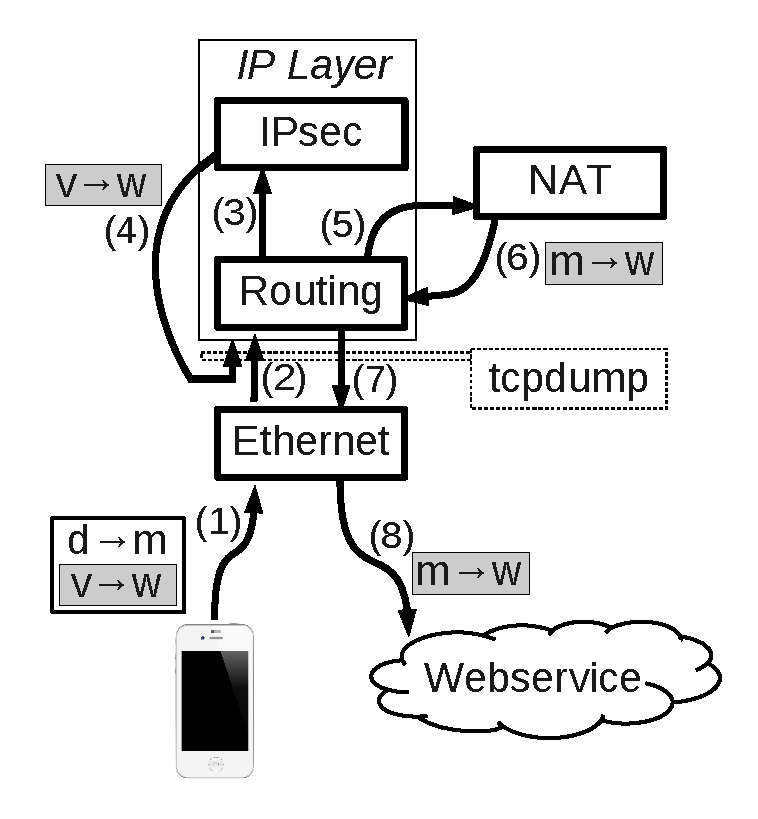
\includegraphics[width=0.47\columnwidth]{figures/packet-monitoring-a.pdf}}
  \hspace{0.05\columnwidth} \subfloat[Packet to mobile
  device. \emph{Tcpdump can capture packets at step
    (2)~w~$\rightarrow$~m and (7)~m~$\rightarrow$~d, however it is
    cannot log the packet
    w~$\rightarrow$~v.}]{\label{fig:packet-monitor-b}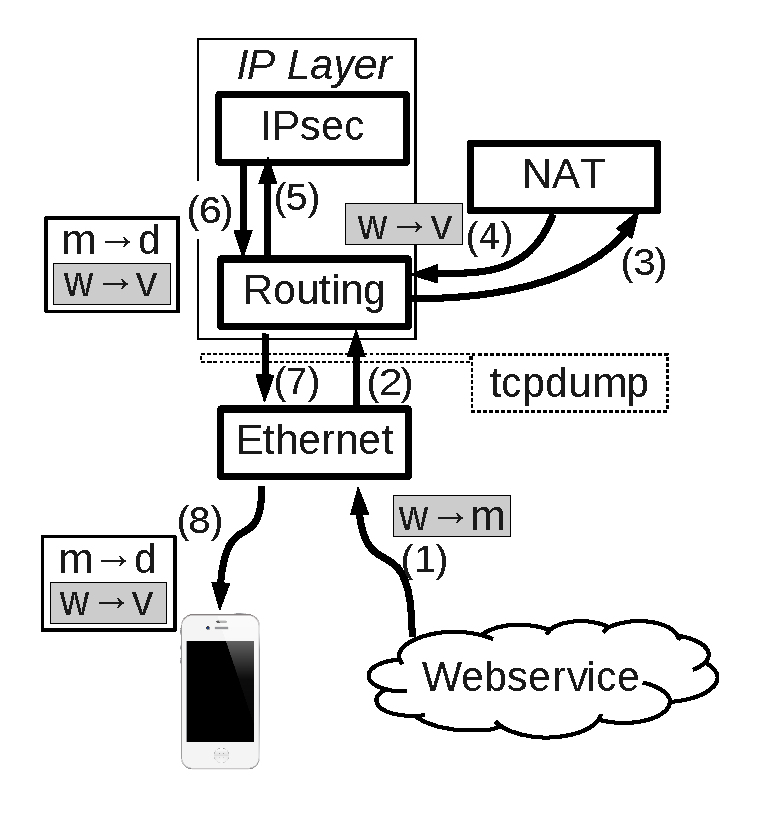
\includegraphics[width=0.47\columnwidth]{figures/packet-monitoring-b.pdf}}
  \newline \subfloat[Packet from mobile device. \emph{Tcpdump
    monitoring packets on the tun device can capture packets at step
    (5)~v~$\rightarrow$~w, and
    (6)~v'~$\rightarrow$~w.}]{\label{fig:packet-monitor-c}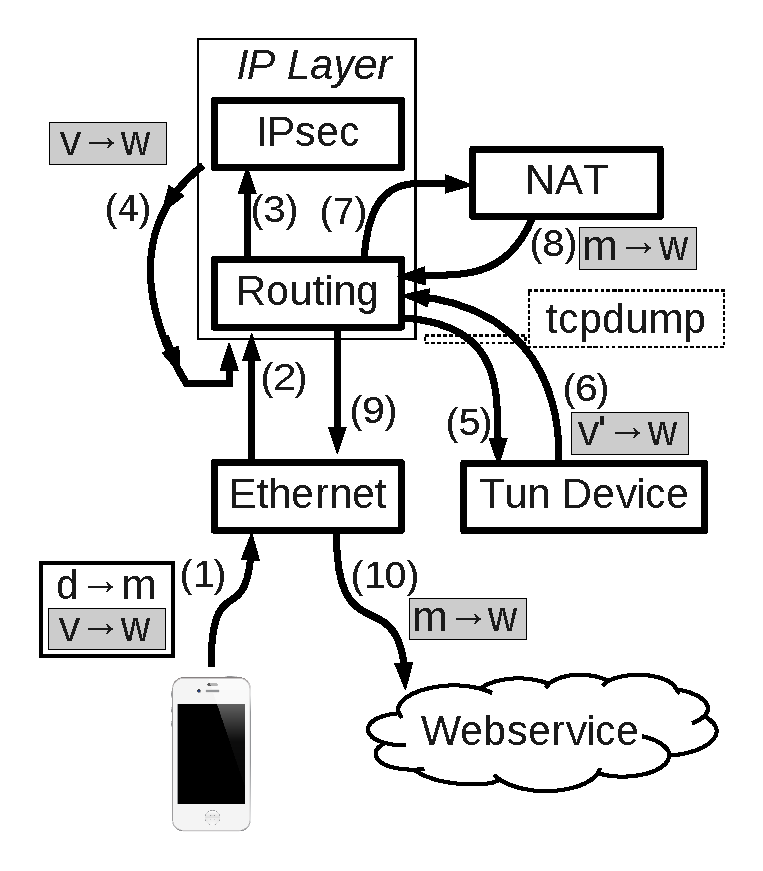
\includegraphics[width=0.47\columnwidth]{figures/packet-monitoring-c.pdf}}
  \hspace{0.05\columnwidth} \subfloat[Packet to mobile
  device. \emph{Tcpdump monitoring packets on the tun device can
    capture packets at step (5)~w~$\rightarrow$~v', and
    (6)~w~$\rightarrow$~v.}]{\label{fig:packet-monitor-d}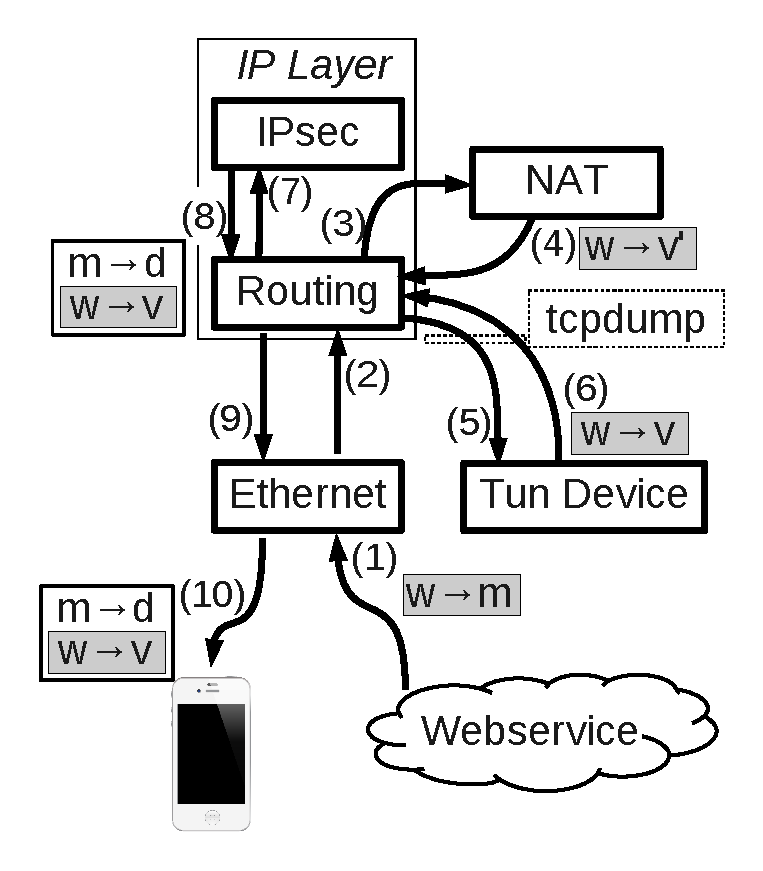
\includegraphics[width=0.47\columnwidth]{figures/packet-monitoring-d.pdf}}
  \newline
\begin{small}
\begin{tabular}{|c|p{0.8\columnwidth}|}
\hline
Symbol & Description \tabularnewline
\hline
d & IP address of the mobile device assigned by its ISP. \tabularnewline
m & IP address of the \platname server. \tabularnewline
w & IP address of the server providing the Web service. \tabularnewline
(i) & The i-th step of packet processing. \tabularnewline
\fbox{a $\rightarrow$ b} & Packet with source IP \emph{a} and destination IP \emph{b}. \tabularnewline
v & IP address of the mobile device in the VPN tunnel. \tabularnewline
v' & Temporary IP address of the mobile device used to send the packet
to the TUN device. \tabularnewline

\hline
\end{tabular}
\end{small}
\end{center}
\caption{Packet monitoring in the \platname{} box.}
\label{fig:packet-monitoring}
\end{figure}

% %start the discussion of the technical details. TO REWRITE
% The IPsec implementation in the Linux kernel is not suitable to
% traffic monitoring when the server running the VPN daemon is used to
% proxy Internet traffic.  A VPN Proxy, apart from serving VPN tunnels,
% relies on NAT to proxy Internet traffic.  When a mobile device
% establishes a VPN tunnel, the VPN server assigns it assigned a private
% IP address.  The mobile device therefore has two IP addresses, a
% private address assigned by the VPN server, and a public IP address
% assigned by the service provider.  The public IP address is used only
% to communicate with the VPN server while all other communication uses
% the private IP address.  Therefore all the traffic that would have
% used the public IP address when the VPN tunnel was not present, now
% uses the private IP address.  These packets that use the private IP
% are encapsulated and encrypted using IPsec and sent to the VPN server.
% The VPN server decapsulates these packets before forwarding them.
% Before forwarding the packet, the VPN server must perform NAT because
% these private IP address cannot used in the Internet.  The use of NAT
% and IPsec implies that the forwarding each packet by the server is
% governed by two rules: one rule to enforce IPsec encryption and
% decryption of packets that contain the public IP of the mobile device,
% and the other that enforces NAT for packets with the private IP
% address.

% An association between the mobile device and a packet is possible only
% if the packet encapsulated within an IPsec packets is monitored in the
% clear.  However, the current implementation of NAT and IPsec makes
% this association of packets with the mobile devices non-trival.  A
% packet from the mobile device, encrypted using IPsec, needs to be
% decrypted before undergoing NAT.  As shown in
% \fref{fig:packet-monitoring-problem}, because the IPsec computations
% take place after the NAT computations, the kernel loops the packet
% back to the IP layer after decryption.  This looping allows the packet
% monitor to observe the IPsec packet before and after
% decryption\footnote{A similar operation takes place if the mobile
%   devices communicate with each other over P2P however we do not
%   discuss this scenario due to lack of space.}.  When multiple flows
% pass through the VPN server, the packet monitor can use the private IP
% address to associate the packets with the mobile device.  Once the NAT
% operation is performed the packet is forwarded via the network card.
% When the network card receives a packet intended for the mobile
% device, as shown in \fref{fig:packet-monitoring-problem}, the packet
% first undergoes NAT followed by IPsec encryption.  The encrypted
% packet is then sent to the mobile device.  Because the packet is not
% looped through the packet monitor before encryption, the packet
% monitor is not able to see the packet after NAT and before encrpytion.
% This implies without any modifications, any off the shelf packet
% monitor shall fail to associate the packets destined for mobile
% devices with the corresponding mobile device.

\subsubsection{Interposing on Traffic on MobiScope}
\label{sec:modif-traffic-mobiscope}

\begin{figure}
\begin{center}
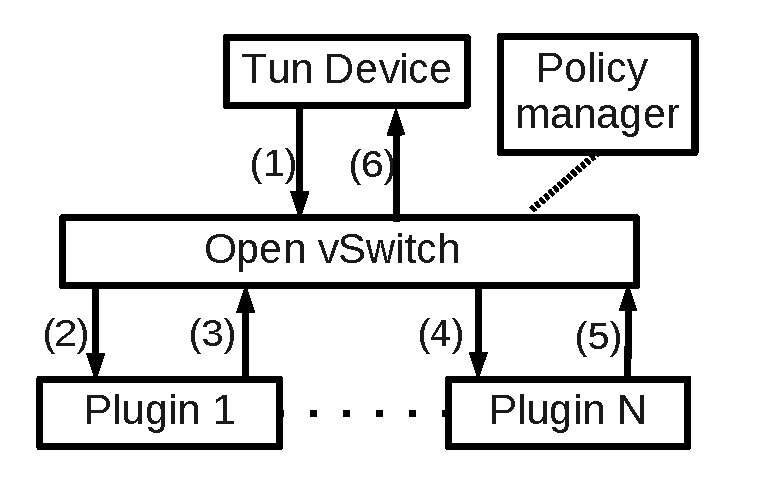
\includegraphics[width=0.8\columnwidth]{figures/packet-monitoring-plugin.pdf}
\end{center}
\caption{Plugin Infrastructure on \platname.}
\label{fig:packet-monitoring-solution}
\end{figure}

A key limitation of previous approaches to measuring mobile 
network traffic is that the contents of encrypted (SSL) traffic 
are unavailable for analysis. Of course, SSL rightfully provides 
authentication and protects user privacy from eavesdroppers; 
however, as increasing amounts of Web traffic flow over HTTPS, 
we lose the ability to understand how to optimize such traffic. 
This has implications both for performance (page speed optimizations) 
and privacy (PII leakage over secure channels). In this section, 
we describe how \platname{} allows us to analyze the contents 
of SSL flows generated by mobile devices. 

\noindent\textbf{Plugin infrastructure.} Figure~\ref{fig:packet-monitoring-solution} shows how we use 
our virtual network interface (TUN) to support a plugin
infrastructure for \platname. Each plugin takes as input a 
network flow and outputs a network flow (potentially empty). 
When a packet is received at the TUN
device, it is sent to a software-defined switch~\cite{Openvswitch} that 
determines the ordered set of plugins that flows will traverse. 
This order is configured by a policy manager, which determines 
the set of plugins that should operate on each flow. After the last 
plugin is traversed, the network flow is sent out through the TUN device 
to the Internet. 

Plugins can be used for many different purposes such as ad blocking, 
analyzing PII leakage or page speed optimization. In the following, we 
describe how we use a plugin to enable SSL traffic decryption using 
the \platname{} plugininfrastructure. 


\noindent\textbf{Example plugin: SSL bumping.} 
First, we note that our VPN proxy implementation uses a self-generated 
\platname{} root certificate that is used to sign all subsequent certificates 
issued to participating mobile devices. This allows us to perform SSL 
traffic decryption, using the Squid proxy's SSL bumping\tbd{AR: give a 
reference} feature, which is essentially a man-in-the-middle operation 
on the secure connection.\footnote{Note that for privacy reasons we do not 
decrypt traffic generated by human subjects; rather, we use this for controlled 
experiments in the lab setting.} Specifically, when the mobile device connects 
to a service supporting SSL, the proxy impersonates the service using a forged certificate signed
with the root certificate of the \platname{} platform. Then the proxy
establishes an SSL connection with the intended target, impersonating a mobile
device. Using the traffic dumped by the tcpdump process as shown in
Figures~\ref{fig:packet-monitor-c} and \ref{fig:packet-monitor-d}, and
using the private key generated by the squid proxy to communicate with
the mobile device, we can decrypt all SSL traffic. We note that when
traffic is not encrypted using SSL, the proxy simply acts as a
transparent proxy. 

This approach will fail for any app that does not trust certificates 
signed by anything other than a well known root authority. 
Surprisingly, this is rarely the case. Whereas the
Twitter application and the Firefox browser prevent SSL bumping by
validating the root certificate, Google Chrome, Safari, the Facebook
application, the Google+ application, the default mail clients, and
advertisement services do not check the validity of the root
certificate. This enables our approach to provide visibility into 
secure channels established with a wide range of popular apps. We will discuss
further this issue in Section~\ref{sec:classification}. 

% \begin{figure}
% \begin{center}
% \includegraphics[width=0.8\columnwidth]{figures/tun-device.pdf}
% \end{center}
% \caption{Tun-tap device to loop packets for packet monitoring.}
% \label{fig:packet-monitoring-solution}
% \end{figure}

% To monitor the packets that are encapsulated within IPsec packets we
% route the packets through a tun-tap device before encryption and after
% decryption.  As shown in \fref{fig:packet-monitoring-solution},

% \subsubsection{Transparent Proxy}
% \label{sec:platform-transparent-proxy}


\subsection{Limitations and Deployability}
\label{sec:addit-limit}

\platname{} provides a scalable way to achieve pervasive, portable 
and passive monitoring of network traffic from mobile devices. In 
this section, we discuss several issues that impact the coverage 
and deployability of our approach. Note that these limitations have 
not significantly impacted our ability to measure mobile networking 
traffic or to deploy our approach to users.

\subsubsection{Limitations}

\drc{Add text about monitoring only one interface.}

\noindent\textbf{At most one tunnel.} Currently iOS and Android 
support exactly one VPN connection at a time. This allows \platname{} 
to measure traffic over either WiFi or cellular interfaces, but not both at once. 
The vast majority of traffic uses only one of these interfaces, 
and that interface uses the VPN.

\noindent\textbf{Proxy location.} All traffic is proxied through a \platname{} box, thus the Web
services will see the \platname{} box address as the end-point and not
the mobile device. This might have an impact in case of Web service
tailoring the answer according to the IP address of the mobile device
(e.g., in case of localization). The biggest problem is when a Web
service deny access to some geographic area, but this problem can be
worked around by installing a \platname{} box on a local (to the Web
sevice) machine.

\noindent\textbf{ISP support.} Some ISPs block VPN traffic. In that case it is not possible
to use the \platname{} platform from a mobile device connected to
such an ISP. There are few ISPs blocking VPN traffic, and there is a
strong incentive to enable VPN traffic in order to attract
professional clients. 

\noindent\textbf{Limited ISP characterization.} \platname{} cannot detect traffic 
differentiation or any other techniques that ISPs use to interpose on network 
traffic using deep packet inspection (such as
advertisement insertion \tbd{AR: give a reference}) or optimization
(such as traffic compression \tbd{AR: give a reference}). This is because the traffic between mobile devices and \platname{}
is encrypted.

\noindent\textbf{IPv6.} \platname{} cannot be currently used on networks using IPv6
because IPv6 is not fully supported by mobile devices. Indeed, we
observe that though iOS and Android support IPv6 they currently do not
support IPv6 traffic through VPN tunnels.

\tbd{Should we use the tripewire experiment? Currently the description
looks like a very small contribution, and it does not bring much to
the discussion. }

\subsubsection{Deployability}
\platname{} uses standard and often open-source software to manage and
record traffic from mobile devices, making it easy to deploy to users
and servers. However, a key question is whether the system is
sufficiently efficient to minimize its impact on both controlled and
in-the-wild experiments. We show empirically that the overheads are
reasonable, and provide a brief discussion of incentives for users to
adopt our system for in-the-wild experiments.

We identify the following key aspects of user-perceived inefficiency from 
proxying their network traffic through \platname{}: 
\begin{itemize}
\item \textbf{Establishment delay.} We made a simple set of 50 VPN establishments on both iOS (on an
iPhone 5 running iOS 6.1) and Android (on a Galaxy Nexus running
Android 4.2), and for both \wifi{} and cellular connections. For
Android, we found maximum VPN establishment of 0.81 second on \wifi{}
and of 1.59 second on cellular. For iOS that uses the older IKEv1, the
VPN establishment takes longer: we observe a maximum of 2 seconds on
\wifi{} and 2.18 seconds on cellular.  In summary, for most long term
traffic monitoring experiments, the VPN establishment delay is
negligible. \drc{median? AL: I removed the median to reduce too many
  references to numbers. In that case, the max is enough to support
our argument.}
\item \textbf{Encapsulation overhead -- data consumption.} \platname{} uses IPsec for datagram encryption, thus there is
an encapsulation overhead for each packet exchanged between the mobile
device and the \platname{} box. To evaluate this overhead, we logged
for 30 days and 25 mobile devices the size of all IPsec packets and of
the encapsulated packet. We observe a maximum increase in the packet
size due to the IPsec encapsulation of 12.8\%. Within the scope of the
traffic monitoring experiments performed with \platname{}, the impact
of this overhead is negligible. However, in case of experiments with a
limited cellular data plan, this overhead must be taken into account.

\item \textbf{Encapsulation overhead -- power consumption.}
To establish and maintain a VPN tunnel, the mobile devices need
additional resources that translate into a larger battery drain during
experiments. To evaluate this battery consumption due to the VPN, we
used a power meter to measure the draw from a Galaxy Nexus running
Android 4.2. We run 10-minute experiments with and without the VPN
enabled. For each experiment, we generated an intensive activity such
as Web searches, map searches, Facebook interaction, e-mail and video
streaming. We found that the VPN leads to a 10\% power overhead. 

We used a power meter on an Android device only because power
measurements require physical access to the battery for a device,
which is not feasible for iOS devices. For iOS devices we conducted
an experiment using video streaming to drain a fully charged battery with 
and without the VPN enabled. We again found approximately 10\% power overhead. 

In summary, the power overhead is low enough to run long experiments
using mobile devices on \platname. To further reduce this overhead (which 
is primarily for cryptographic operations), we are investigating using NULL 
encryption (\ie no encryption) for users that do not need 
the additional privacy enabled by our VPN proxy.

\end{itemize}

\noindent\textbf{Incentives.} \platname{} is a fantastic platform for
controlled experiments. However, it is also important to measure
traffic from real users, so we must provide an incentive for them to
use the platform. We have developed a variety of user incentives that
can offset the costs of \platname{}; here, we name a few of the most
interesting ones.\footnote{We have implemented most of these examples,
  but their details are beyond the scope of this paper.} For example,
we can provide users with fine-grained views of privacy leaks from
their applications, and allow them to enable a \platname{} plugin that
blocks Personally Identifiable Information (PII). In addition, we are
investigating the opportunities for page speed optimization. Last, we
have implemented opt-in device-wide ad-blocking, which can reduce the
volume of costly cellular traffic transferred by a device.


%
%
%VPN establishment delay,
%data consumption overhead due to the VPN encapsulation, power
%consumption overhead on the mobile device. Then we discuss additional
%limitations such as the one due to the encryption of all the traffic
%between the mobile device and the \platname{} box, encryption
%preventing the access ISP to perform traffic modification and
%optimization. 
%% Finally, we discuss the scalability of a single
%% \platname{} box.
%
%\subsubsection{VPN Establishment Delay}
%To establish a VPN tunnel, the mobile device and the \platname{} box
%must negotiate, which takes time. iOS devices use IKEv1 to establish VPN
%tunnels, whereas Android devices use the more recent and faster IKEv2.
%
%% The iOS devices use IKEv1 to manage the VPN tunnels while Android
%% devices support both IKEv1 and IKEv2.  To establish the VPN tunnel,
%% IKEv1 requires a total of 16 packets to be exchanged between the
%% mobile client and the VPN server while IKEv2 requires 4 packets.
%% \platname uses IKEv2 for Android devices while IKEv1 is used for iOS
%% devices.
%
%We made a simple set of 50 VPN establishments on both iOS (on an
%iPhone 5 running iOS 6.1) and Android (on a Galaxy Nexus running
%Android 4.2), and for both \wifi{} and cellular connections. For
%Android, we found maximum VPN establishment of 0.81 second on \wifi{}
%and of 1.59 second on cellular. For iOS that uses the older IKEv1, the
%VPN establishment takes longer: we observe a maximum of 2 seconds on
%\wifi{} and 2.18 seconds on cellular.  In summary, for most long term
%traffic monitoring experiments, the VPN establishment delay is
%negligible. \drc{median?}
%
%% To measure the time required to establish a VPN tunnel, we performed
%% controlled tests using one Android device and an iPhone 5.  We
%% performed these tests from two different locations based in the same
%% city in which the server was deployed.  OUr tests involved
%% \tbdv{number} of VPN tunnel creation over a time period of \tbdv{}
%% hours.  When the Android device used \wifi to establish the VPN
%% tunnel, we observe a median connection establishment time of 0.62
%% seconds from both locations with a maximum of 0.81 seconds and 0.79
%% seconds respectively.  When the Android device used cellular networks
%% to establish the tunnel, the median connection establishment time was
%% 0.81 seconds from both locations with a maximum of 1.59 seconds.
%
%% Compared to the Android device, the iOS devices required a larger
%% amount of time to establish the connection because it relies on a an
%% older key authentication protocol.  From the two Wi-Fi networks, to
%% establish the VPN tunnel, the iOS device required 1.60 seconds and
%% 1.34 seconds with a maximum of 2.0 seconds and 1.48 seconds
%% respectively; in the case of cellular networks we observed a median of
%% 1.80 seconds and 1.65 seconds with a maximum of 2.18 seconds and 1.87
%% seconds respectively. \drc{This needs to go in a table, since it is
%%   impossibly dense.}
%
%% \tbd{In summary, we observe that because iOS devices use an older key
%%   exchange protocol they can take up to twice as much time as Android
%%   devices to establish the VPN tunnel.  Any more insights .. The
%%   tunnel establishment times in the order of 2 seconds implies that
%%   \platname can have a significant latency overhead if VPN tunnels are
%%   established periodically for short tests.}
%
%\subsubsection{Data Consumption Overhead}
%\platname{} uses IPsec for datagram encryption, thus there is
%an encapsulation overhead for each packet exchanged between the mobile
%device and the \platname{} box. To evaluate this overhead, we logged
%for 30 days and 25 mobile devices the size of all IPsec packets and of
%the encapsulated packet. We observe a maximum increase in the packet
%size due to the IPsec encapsulation of 12.8\%. Within the scope of the
%traffic monitoring experiments performed with \platname{}, the impact
%of this overhead is negligible. However, in case of experiments with a
%limited cellular data plan, this overhead must be taken into account. 
%
%
%% IPSec encapsulation slightly inflates packet sizes, in addition to
%% preventing carrier middleboxes from applying their own compression.
%% We measured the overhead of the tunnel in terms of data overhead from
%% IPsec headers and keep-alive messages, finding that it ranges from
%% 8--12.8\%.
%
%% To compute the increase in the amount of bytes transferred due to
%% encapsulation and the keep-alive messages, we log the packet lengths
%% of the encrypted packets (IPsec packets) exchanged by our \platname
%% servers and the mobile clients.  We performed this packet capture for
%% 30 days during which 25 devices tunneled their traffic via \platname.
%% During this time interval we also log the packet length of the packets
%% encapsulated within the IPsec packets.  During this 30 day period we
%% observe that the median of the increase to be 8.31\%, with a maximum
%% increase of 12.8\%.
%
%% \tbd{In summary, we observe a maximum overhead of 12.8\% increase in data consumption. We believe the costs of this overhead are minimal compared to the cost of warrant voiding the device.}
%
%\subsubsection{Power Consumption Overhead}
%To establish and maintain a VPN tunnel, the mobile devices need
%additional resources that translate into a larger battery drain during
%experiments. To evaluate this battery consumption due to the VPN, we
%used a power meter to measure the draw from a Galaxy Nexus running
%Android 4.2. We run 10 minutes experiments with and without the VPN
%enabled. For each experiment, we generated an intensive activity such
%as Web searches, map searches, Facebook interaction, e-mail and video
%streaming. We found that the VPN leads to a 10\% power overhead. 
%
%We used a power meter on an Android device only because power
%measurements require physical access to the battery for a device,
%which is not feasible for iOS devices. For iOS devices we made
%simpler experiments consisting in draining a fully charged battery with
%a video streaming with a without the VPN enabled. We found also around
%a 10\% power overhead. 
%
%In summary, the power overhead is low enough to run long experiments
%using mobile devices on \platname. 
%
%% \footnote{We use Android because power measurements
%%   require physical access to the battery for a device, which is not
%%   feasible for iOS devices. We found similar results when testing the
%%   time to discharge an iOS device while streaming video with and
%%   without a VPN connection.}
%
%% We found that VPN proxying imposes approximately 10\% power overhead
%% compared to direct traffic. To test the additional power consumption
%% from using a VPN proxy, we used a power meter to measure the draw from
%% a Galaxy Nexus running Android 4.2.\footnote{We use Android because
%%   power measurements require physical access to the battery for a
%%   device, which is not feasible for iOS devices. We found similar
%%   results when testing the time to discharge an iOS device while
%%   streaming video with and without a VPN connection.} While
%% instrumented, we conducted 10-minute experiments where we scripted
%% device usage with and without a VPN enabled. The activities included
%% Web searches, map searches, Facebook interaction, e-mail and video
%% streaming.
%
%\subsubsection{Additional Limitations}
%

% To understand whether traffic interposition by ISPs is frequent, we
% made a dedicated experiment using tripewires\tbd{cite the paper}.  In
% particular, we exploit Android's support for apps providing VPN
% services; instead of establishing a secure connection we simply
% forward traffic to a proxy server without additional encryption. In
% this way, the mobile device's ISP can inspect the contents of all
% non-SSL traffic and interpose accordingly.  Note that one limitation
% of this approach is that the ISP will see the destination for all
% network traffic is our proxy server (instead of the original
% destination), which could impact how ISPs treat the corresponding
% traffic.

% T-Mobile  AT&T 1000 first alexa rank, in France Orange and Free. 

% VPN proxying via secure tunnels prevent ISPs from inspecting or
% interposing on network traffic, thus preventing us from measuring this
% behavior. To understand ISP interference with mobile Internet traffic,
% we additionally support measurement using an \emph{insecure}
% transparent proxy.  In particular, we exploit Android's support for
% apps providing VPN services; instead of establishing a secure
% connection we simply forward traffic to a proxy server without
% additional encryption. In this way, the mobile device's ISP can
% inspect the contents of all non-SSL traffic and interpose accordingly.
% Note that one limitation of this approach is that the ISP will see the
% destination for all network traffic is our proxy server (instead of
% the original destination), which could impact how ISPs treat the
% corresponding traffic.


% \tbd{In summary, despite these shortcoming we believe that \platname can be used for realistic measurements of mobile Internet traffic.}




%%% Local Variables: 
%%% mode: latex
%%% TeX-master: "main.tex"
%%% End: 


\section{Evaluation}
\label{sec:eval}
This section evaluates \meddle in terms of overhead, visibility into network traffic and 
the ability to map network traffic to the apps that generated it. We use the results in 
this section to inform the applications we build in \S\ref{sec:characterize-app} and \S\ref{sec:isp-behavior}.

\subsection{Methodology}
\label{sec:dataset}
Using \platname, we collected full packet traces from Internet activity generated by
mobile devices. We use this data to study how to map monitored traffic to applications, and to
analyze PII leakage. Below, we describe our data-collection methodology, which consists of
1) controlled experiments in a lab setting and 2) IRB-approved ``in the wild'' measurements 
gathered from real users during seven months.


\subsubsection{Controlled Experiments with Apps}
\label{sec:dataset-contr-exper}
Our goal with controlled experiments is 1) to obtain ground truth information 
about network flows generated by apps and devices, and 2) characterize the 
network activity for a large variety of apps in a lab setting. We use 
this data to understand how to model apps' network behavior, how to map network flows 
to the app that generated them and how to identify PII in those network flows. 

\noindent\textbf{Device setup.} We conducted our controlled experiments using two Android 
devices (running Android 4.0 and 4.2) and an iPhone running iOS 6. We start each set of controlled experiments
 with a factory reset of the device to ensure that software installed by previous 
 experiments cannot impact the network traffic generated by each device. 
 Then we connect the device to \platname{}  and begin
the experiment. 


\noindent\textbf{SSL bumping.} 
We use SSL bumping only in controlled experiments where \emph{no user traffic is intercepted}.
%, using a plugin to enable % SSL traffic decryption. 
We are also designing a study for IRB approval in which users can opt in to use SSL bumping for obfuscating PIIs in their SSL traffic.

\noindent\textbf{Manual tests.} We manually test the
100 most popular free Android apps in the \emph{Google Play} store and 209
iOS apps from the iOS App store on April 4, 2013. For each
app, we install it, enter user credentials %for the account 
if relevant, interact with it for up to 10 minutes, and uninstall
it. This allows us to characterize real user interactions with popular apps
in a controlled environment.  
We enter unique and distinguishable user credentials when 
interacting with apps to easily extract the corresponding PII from 
network flows (if they are not obfuscated). We use the same technique 
to test malware apps (\S\ref{subsec:malware}).

\noindent\textbf{Automated tests.} The second set of controlled experiments consist of fully-automated
experiments on 732 Android apps from a free,
third-party Android market, \emph{AppsApk.com}~\cite{appsapk}.
We perform this test because Android users can install
\emph{Third-party apps} without rooting their device. 
% that are not available on the
%\emph{Google Play} store, 

Our goal is to understand how these apps differ from those in the standard \emph{Google Play} 
store, as they are not subject to Google Play restrictions.
%\tbd{Is there different constraints on this free market, AR: They do not have paid application. All apps must be free.}
We automate experiments using \emph{adb} to
install each app, connect the device to the \meddle platform, and
start the app. Then we use \emph{Monkey}~\cite{adbmonkey}, an app-scripting 
tool, to perform a series of  approximately 100,000 actions that include
random swipes, touches, and text entries.  Finally, we use adb to
uninstall the app and reboot the device to forcibly end any
lingering connections. This set of experiments is limited to
Android devices because iOS does not provide equivalent 
scripting functionality. 
%\tbd{Are they stores from which you can download apps for non jail-broken iOS devices? DC: No.}

\subsubsection{In Situ Study}
\label{sec:dataset-wild-measurements}

The controlled experiments in the previous section provide us with 
ground-truth information for a large number of apps running in a controlled 
setting for a short period of time. To understand the network behavior of 
devices with real users ``in the wild'' over longer time periods, we conducted 
an IRB-approved measurement study with a small set of subjects, from 
Oct. 15, 2012 to Sep. 1, 2013.\footnote{The measurement study is ongoing, we report a subset of results.}

Our measurement data was collected from 26 devices: 10 iPhones, 4 iPads, 1 iPodTouch, and 11
Android phones.  The Android devices in this dataset include the
Nexus, Sony, Samsung, and Gsmart brands while the iPhone devices
include one iPhone~3GS, four iPhone~5, and five iPhone~4S.  These
devices belongs to 21 different users, volunteers for our IRB approved
study.  This dataset, called \mobWild, consists of 318 days with data; the number of 
days for each user varies from 5 to 315 with a median of 35 days.  For privacy reasons, the
SSL-Bumping plugin is \emph{disabled} for all measurements involving
real users.


\subsection{Overheads}
\noindent\emph{Network Latency.}
We first test indirection overhead from mobile networks to a \meddle instance. In the 
US with EC2, delays from mobile-network egress points to EC2 nodes are on generally less than 10\,ms. 
For other networks, we will achieve similarly low indirection overhead by placing instances in a cloud/hosting 
provider near subscribers and use DNS redirection (\eg via Amazon's Route 53) to direct clients to nearby instances. 

The other source of network delays is connection establishment time, incurred once per session. We measured 
50 VPN-connection establishment times on both iOS (iPhone 5 / iOS 6.1) and Android (Galaxy Nexus /
Android 4.2), for \wifi{} and cellular connections. We conduct tests in rapid succession to ensure the radio is in the high power state.
The \meddle server was running on a university network. 
For Android (using IKEv2), the maximum establishment time was 0.81 seconds on \wifi{} and 1.59 seconds on cellular. 
For iOS (using IKEv1), the connection takes longer due to the older protocol version: we observe a maximum of 2 seconds on \wifi{} and 2.18 seconds on cellular. 
Because each VPN session supports many flows, the amortized cost of connecting is  small. 
%\tbd{Cite results from latency to home gateways based on DSL results in PAM and IMC.}
%\tbd{Address comments in conext review on latency}

\noindent\emph{Power Consumption.}
Mobile devices expend additional power to establish, maintain and encrypt data for a VPN tunnel. 
To evaluate the impact on battery, we used a power meter to measure the draw from a Galaxy Nexus running Android 4.2. 
We run 10-minute experiments with and without the VPN enabled. 
For each experiment, we used an activity script that included Web and map searches, Facebook interaction, e-mail and video
streaming. 
The VPN leads to a 10\% power overhead. 
For iOS devices, we relied on the battery readings provided by iOS because we cannot attach a power meter directly to the battery.
We again found an approximately 10\% power overhead of using VPNs when we drained a fully charged battery while performing the operations performed during the tests for Android devices.  

%\item 
\noindent\emph{Traffic Volume.}
\meddle relies on IPsec for datagram encryption, thus there is an encapsulation overhead for each tunneled packet. 
To evaluate this overhead, we use 30 days of data from 25 devices that to compare encapsulated and raw packet sizes. 
We observe a maximum encapsulation overhead of 12.8\% (average approximately 10\%). 
For users that have limited data plans and consume most of their quota per month, this can have 
a significant impact. We note that this is partially offset by \meddle services such as content filtering and 
connection blocking. % and optimizations such as transcoding and compression. 

\noindent\emph{Scalability.} We currently use Amazon EC2 to support users at our cost. 
Without exploring opportunities for economies of scale, we estimate that 
it will cost less than a penny (\$0.0084) per user per day. At this cost, we can support up to 
10,000 users with research funds. If \meddle were to become extraordinarily popular, it would 
cost each user approximately a quarter per month to pay their own way. By comparison, 
data plans in the US tend to cost \$30-\$90 per month -- more than two orders of magnitude larger.

\subsection{Meddle Visiblity}

%We now highlight key features of the \mobWild dataset. 
We now use data gathered from users to demonstrate that there is a need for a platform like \meddle that provides a comprehensive view of Internet traffic from mobile devices. 
Note that due to the relatively small number of users in our study, we do not attempt to  
draw strong and generalizable conclusions. 

\noindent\textbf{Observation 1: \emph{End-host instrumentation provides a more complete view of 
Internet traffic from mobile devices.}} We infer the access technology (WiFi or cellular) for 
each session with the AS description from a \emph{WHOIS} lookup for each IP address used by a mobile device.
Based on this classification, the \mobWild dataset consists of traffic from 65 distinct ASes, of which 8 are cellular ASes and 7 are university networks.

We observe less diversity in cellular ASes compared to \wifi ASes.
During the measurement study, each device connected to our \platname server from at most two distinct cellular ASes. 
In contrast, a median of 4 \wifi ASes were observed per device and for one device we observed traffic from 36 different \wifi ASes spread across 5 countries.
In terms of traffic volumes, collectively our users with cellular connectivity transferred 24-56\% of their traffic over cellular and the remainder over WiFi. 
The key take-away is that, for the users in the \mobWild dataset, we would miss a large fraction of traffic generated by the mobile devices by instrumenting a single cellular carrier or WiFi access point. 
\meddle does not have this limitation.

\noindent\textbf{Observation 2: \emph{\meddle provides visibility into a wide range of traffic patterns}.} 
We use the classification provided by Bro~\cite{bro} to categorize flows as either TCP, UDP, or \emph{other}, along with subcategories HTTP, SSL and DNS.
Table~\ref{tab:summaryIOSAndroidTraffic} summarizes the traffic generated by user devices in our study. 

There are three key take-aways from this table. 
First, Web and SSL traffic dominate the traffic for users in the \mobWild dataset; 91.26\% (137.63 GB) of the traffic volume in the \mobWild dataset is either HTTP or SSL.
Second, there is significant diversity in the usage patterns for users with Android and iOS devices; the fraction of total flows over cellular or \wifi differ significantly for each OS. 
Third, a platform that cannot analyze SSL traffic will miss a large fraction of the traffic.
Indeed, a significant fraction of flows use SSL, which prevents classification using deep packet inspection.
This calls into question the overall effectiveness of traffic optimization approaches that rely on middlebox technologies that interpose on plaintext traffic (\eg page rewriting or downsampling media).
This motivates the need for a platform that not only covers multiple OSes and multiple access technologies but is also capable of intercepting all mobile Internet traffic, including SSL traffic, for the purpose of analysis and interposition. 

\begin{table}
\begin{small}
\begin{center}
\begin{tabular}{|p{0.11\columnwidth}|p{0.14\columnwidth}|r|r|r|r|}
\hline
{\bf IP} & \multirow{2}{*}{\bf Service} & \multicolumn{2}{|c|}{\bf Android} & \multicolumn{2}{|c|}{\bf iOS} \tabularnewline
\cline{3-6}
{\bf Protocol} &           &  \textbf{Cell.}  &  \textbf{\wifi}  &  \textbf{Cell.}  &  \textbf{\wifi}  \tabularnewline
\hline
\multirow{3}{*}{TCP}
       &  HTTP (\%)  & 44.83 & 68.23 & 60.07 & 76.92 \tabularnewline
\cline{2-6}
       &  SSL (\%)   & 44.74 & 20.89 & 36.19 & 14.11 \tabularnewline
\cline{2-6}
       &  other (\%) & 8.26  & 10.10  & 2.74  & 1.33 \tabularnewline
\hline
\multirow{2}{*}{UDP}
       &  DNS (\%)   & 1.31  & 0.58  & 0.64  & 0.38  \tabularnewline
\cline{2-6}
       &  other (\%) & 0.54  & 0.11  & 0.31  & 7.24  \tabularnewline
\hline
 Other &  other (\%) & 0.32  & 0.09 & 0.05  & 0.02  \tabularnewline
\hline
\multicolumn{2}{|c|}{\emph{total (\%)}} & 100.00 & 100.00 & 100.00 & 100.00 \tabularnewline
\hline
\multicolumn{2}{|c|}{\emph{Traffic Volume (GB)}}& 9.57 & 21.10 & 16.61  & 103.52 \tabularnewline
\hline
\multicolumn{2}{|c|}{\emph{\# Flows}}   & 927660 & 761735 & 730209 & 2796130 \tabularnewline
\hline
%\multicolumn{2}{|c|}{\emph{\# Devices}} & 10 & 11 & 10 & 15 \tabularnewline
%\hline
\end{tabular}
\end{center}
\end{small}
\caption{\textbf{Traffic volume (in percentage) of popular protocols and services on Android and iOS devices over cellular and \wifi.}
\emph{TCP flows are responsible for more than 90\% of traffic volume. Traffic share of SSL over cellular networks is more than twice the traffic share of SSL over \wifi.}} 
\label{tab:summaryIOSAndroidTraffic}
\end{table}


%\section{Data Analysis}
%
%In this section, we analyze the network traces gathered by \meddle to 
%1) provide summary statistics of data gathered from our 
%users ``in the wild'' and
%2) develop and evaluate several techniques for mapping network flows to 
%applications, which we will use in subsequent sections to identify privacy 
%leaks and malware.


%An important question for network characterization is which app is responsible for which 
%network flows. As we demonstrate in the following section, previous approaches are insufficient 
%for mapping the majority of apps to their corresponding network flows. We describe 
%several techniques to improve this mapping, and present results for controlled experiments 
%and the \mobWild dataset.

\subsection{Mapping Network Flows to Apps}
%\section{Traffic Classification}
\label{sec:classification-methodology}

Mapping network flows to apps is an important step for determining the origins of potentially costly 
network traffic, and for identifying which apps are responsible for privacy leaks. The following 
sections show that  \emph{previous approaches to mapping passively gathered traffic fail to identify
apps responsible for that traffic most of the time} and that \meddle facilitates a first look at 
determining which apps generate traffic over SSL connections.

%Previous work uses passively gathered data 
%to characterize such traffic, which can be useful for a variety of important topics that include 
%traffic engineering, optimization of network-enabled apps and understanding threats to user privacy. 


% 1) for the users in our study, traffic over WiFi and cellular networks 
%are qualitatively different, and studies that focus on only one technology will miss approximately 
%half of the traffic generated by devices; 

%\subsubsection{Classification of Mobile Apps and Services}

Table~\ref{tab:summaryIOSAndroidTraffic} suggests that apps, OS services, and libraries often rely on HTTP and SSL to exchange data.
%To analyze the behavior of mobile services we need to first associate the observed flows with the applications and the OS services responsible for the flows.
In the following analysis, we focus on identifying the apps, OS services, and other services responsible for these HTTP and SSL flows. 
We use ground-truth data from controlled experiments to show that the previous approach for classification fails 
for most popular apps; we then develop techniques to improve this mapping and apply it to our \mobWild dataset. 

\subsubsection{Improving HTTP Traffic Classification}
In \meddle, we need to know which app is responsible for Internet traffic using only network flow information. This section shows how to use \useragent and \httphost fields to identify the apps and services responsible for HTTP flows. Previous work~\cite{maier:mobtraffic,xu:appusage,falaki:mobileusage,falaki:smartphoneusage} is insufficient -- they use HTTP header fields to identify the \emph{category} of corresponding apps, not the specific app.


\begin{table} 
     \centering
     \begin{small}
     \begin{tabular}{|p{0.05\columnwidth}|p{0.08\columnwidth}|p{0.07\columnwidth}|p{0.08\columnwidth}|p{0.09\columnwidth}|p{0.09\columnwidth}|p{0.09\columnwidth}|p{0.09\columnwidth}|}
        \hline
        {\bf OS}&{\bf Store}&{\bf Apps}&{\bf Gen.}&\multicolumn{2}{|c|}{\bf Host} & {\bf User-}&{\bf Combi-} \tabularnewline
        \cline{5-6}    
             &        &     & {\bf HTTP} & {\bf App. } & {\bf Org.}& \bf{Agent}   & \bf{nation}  \tabularnewline                
        \hline    
        iOS  & Apple  & 209 & 176 & 83 (47.1\%)  &  119 (67.6\%)   &  149 (84.6\%)& 157 (89.2\%) \tabularnewline
        \hline
        And. & Google & 100 & 92  & 41 (44.5\%)  &  54 (58.6\%)    &  21 (22.8\%) &  59 (64.1\%)  \tabularnewline
        \hline    
        And. & Other  & 732 &  365 &  17 (4.6\%) &  79 (21.6\%)    &  52 (14.2\%)  & 83 (22.7\%)  \tabularnewline
        \hline
     \end{tabular}
     \end{small}
     \caption{\textbf{Classification of apps based on \httphost and \useragent.} \emph{ Most iOS apps use dedicated \useragent strings to fetch data over HTTP. A combination of \useragent and \httphost identifies the majority of Android and iOS apps.}}
     \label{tab:classification-success}
\vspace{\postfigspace}
\end{table}

%%
%% No HTTP Traffic from 209 - 38 = 171; 171 + 5 (OS possibly - confirm) = 176  ,
%% 181 unique signature, 7*2 = 14 duplicate (fooducate, fdct). 
%% 174 unique application signatures found
%% 5 UA belonged to OS services, geoservices, applecoremedia, gamedkit, securityd, mmsdk 
%% Ads from 98 - 4 -> 94 labels
%% Rough estimate of HTTP for apps because mapping  -- 414 files without HTTP
%%%
%% In amy dataset, 
%% 132 generate only ad traffic 


\noindent\textbf{Controlled experiments.}
In Table~\ref{tab:classification-success} we present results from our classification study using controlled experiments. To 
the best of our knowledge, we are the first to attempt to use ground-truth information to evaluate the 
effectiveness of app classification using only header data. 
%We begin classification using the \httphost field.

\emph{Classifying with \httphost:}
First, we note that 176 of the 209 iOS apps we manually tested generated HTTP traffic.
Column 5 of Tab.~\ref{tab:classification-success} shows that the \httphost field uniquely identified the corresponding app for 47\% of the iOS apps. 
Each app generated multiple flows, some of which did not contain the app signature in the \httphost field, \eg when contacting ad sites or CDNs. 
Such flows comprised 2\% to 85\% of the traffic volume from the iOS apps used during our measurements. 
The \httphost field also can identify the provider that released an app.
For example, we observed the name \emph{Zynga} in the \httphost field when using \emph{Farmville}, an app created by Zynga.
When testing an app, we noted down the name of its creator as the organization, and we searched this name in the \httphost field in the HTTP flows generated by this app.  
In column 6 of Table~\ref{tab:classification-success}, we see that classification by organization is effective for 67\% of iOS apps. 

We observe similar results for flows from apps in Google Play.
However, for the apps from the Third-party store we observe that the \httphost field is less effective. 
Primarily this is due to the fact that a majority of the apps we tested (about 77\%) were stand-alone services such as games. 
These apps contacted advertisement or or CDN sites that do not uniquely identify the app.
Along with the organizations of the apps we tested, we used the Google Play API~\cite{googleplay:api} to extract the names of the creators (organizations) for the 5000 most popular Android apps on the Google Play store. 

\emph{Classifying with \useragent:} 
We observed a non-empty \useragent string in more than 99.7\% of the HTTP flows from iOS and 90.9\%flows from Android. 
A \useragent string may contain an app identifier and other auxiliary information such as details of the OS~\cite{mozilla:useragentdetection}. 
For example, Yahoo Mail's \useragent string contains the string \emph{YahooMobileMail/1.0}. 
However, some apps use more generic \useragent strings such as \emph{AppleCoreMedia} (streaming video on iOS) or \emph{Dalvik} (generic text for Android). 
To extract the app information, we use regular expressions to filter the auxiliary information from the \useragent and cluster the extracted tokens using the edit distance.

Table~\ref{tab:classification-success} shows that 84.6\% of the 176 iOS apps generating HTTP traffic were correctly identified by their \useragent, which we verified by manual inspection.
In contrast, the \useragent was useful in identifying only 23\% of the Android apps generating HTTP traffic, meaning previous techniques depending solely on the \useragent will fail~\cite{maier:mobtraffic,xu:appusage}. 
For the 27 iOS apps which we failed to identify, we observed signatures for OS services and libraries.
Similarly, the majority of Android HTTP traffic contained flows with the default \useragent (\eg, \emph{Dalvik}).
%Further, for the apps from the third-party store, we observe that the \useragent for ads and analytics libraries such as \emph{Google Analytics} and \emph{Adsense for Mobile} were the most common \useragent after the default \useragent.
% such as \emph{Apple Core Media}, \emph{Game Kit}, \emph{Geo Services}, etc. and signatures of third-party libraries and services such as \emph{Google Analytics} and \emph{Adobe Air}.
%,falaki:mobileusage,falaki:smartphoneusage

\emph{Combination of \useragent and \httphost:} 
In Table~\ref{tab:classification-success}, we observe that the \useragent is more effective for mapping iOS apps while the \httphost is more effective for Android apps; however, neither alone is a complete solution. 
We therefore rely on a combination of \useragent and \httphost to classify HTTP traffic. 
For our classification, we first try to classify the HTTP flow using the \useragent.
We use the \httphost field only if we were unable to extract any useful signature from the \useragent field. 
In Table~\ref{tab:classification-success}, we observe that by using a combination of the \useragent and \httphost we were able to identify 64\% of the Android apps and 89\% of the iOS apps. 
%To fill this gap, we are currently investigating how to use ad-network identifiers to classify apps. 

\begin{figure}
\subfloat[iOS]{\label{fig:http-wordcloud-ios}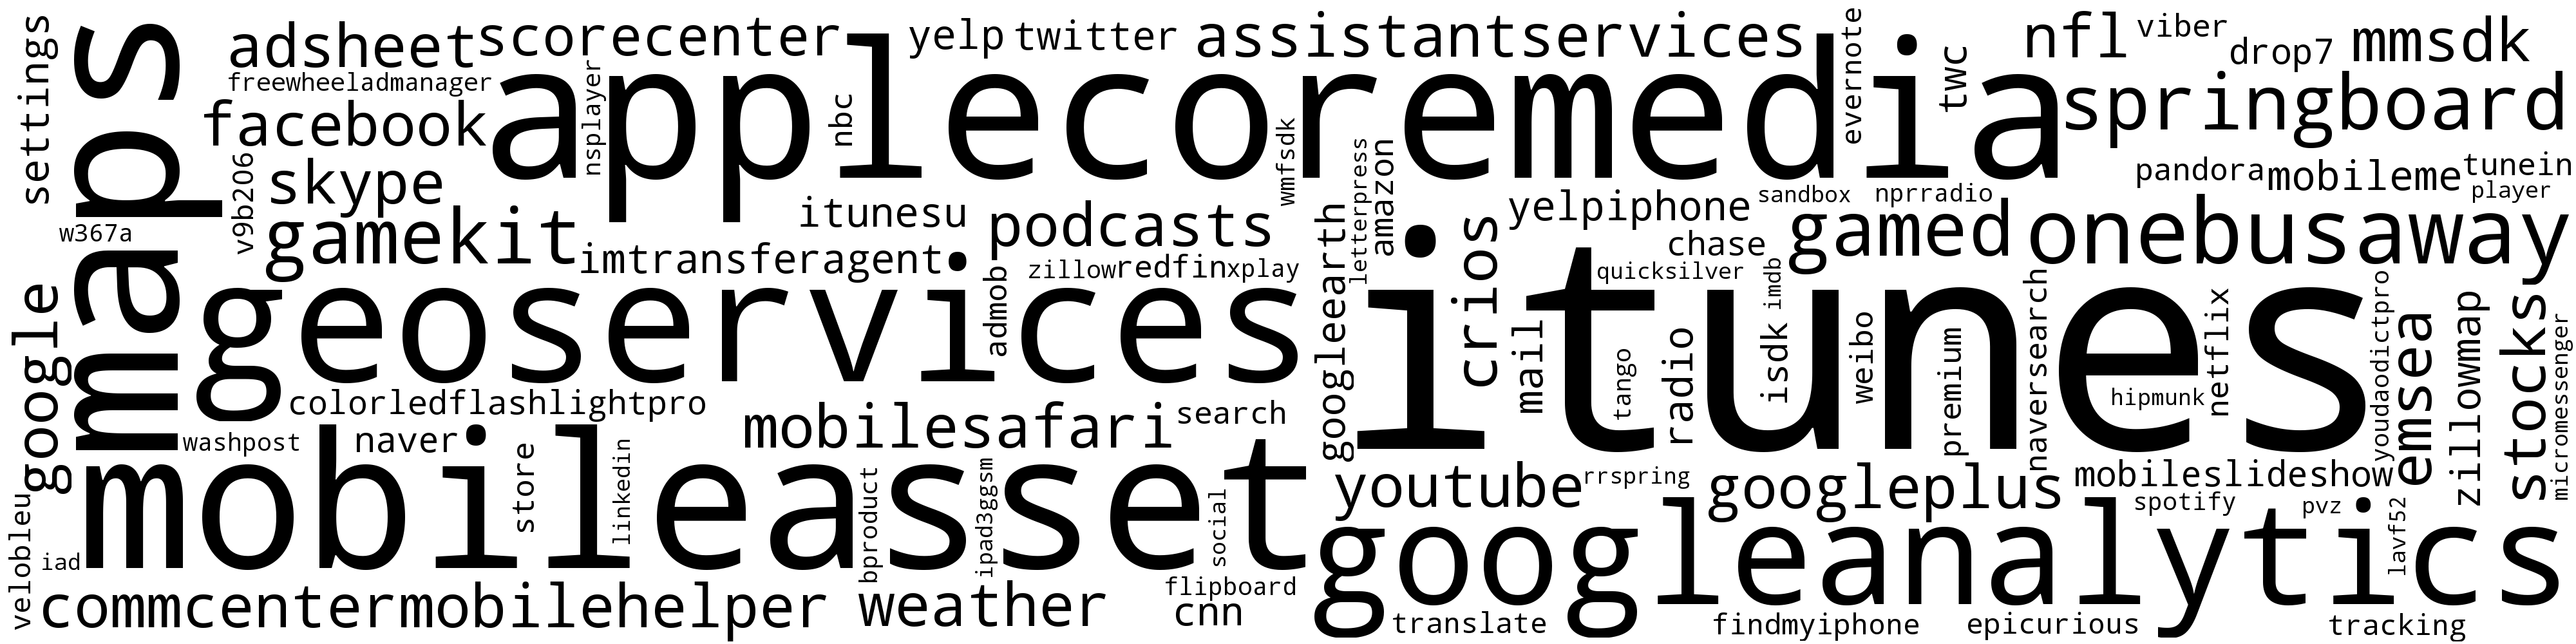
\includegraphics[width=\columnwidth]{figures/wordcloud_useragentsignature_ios_image.png}}\newline
\subfloat[Android]{\label{fig:http-wordcloud-android}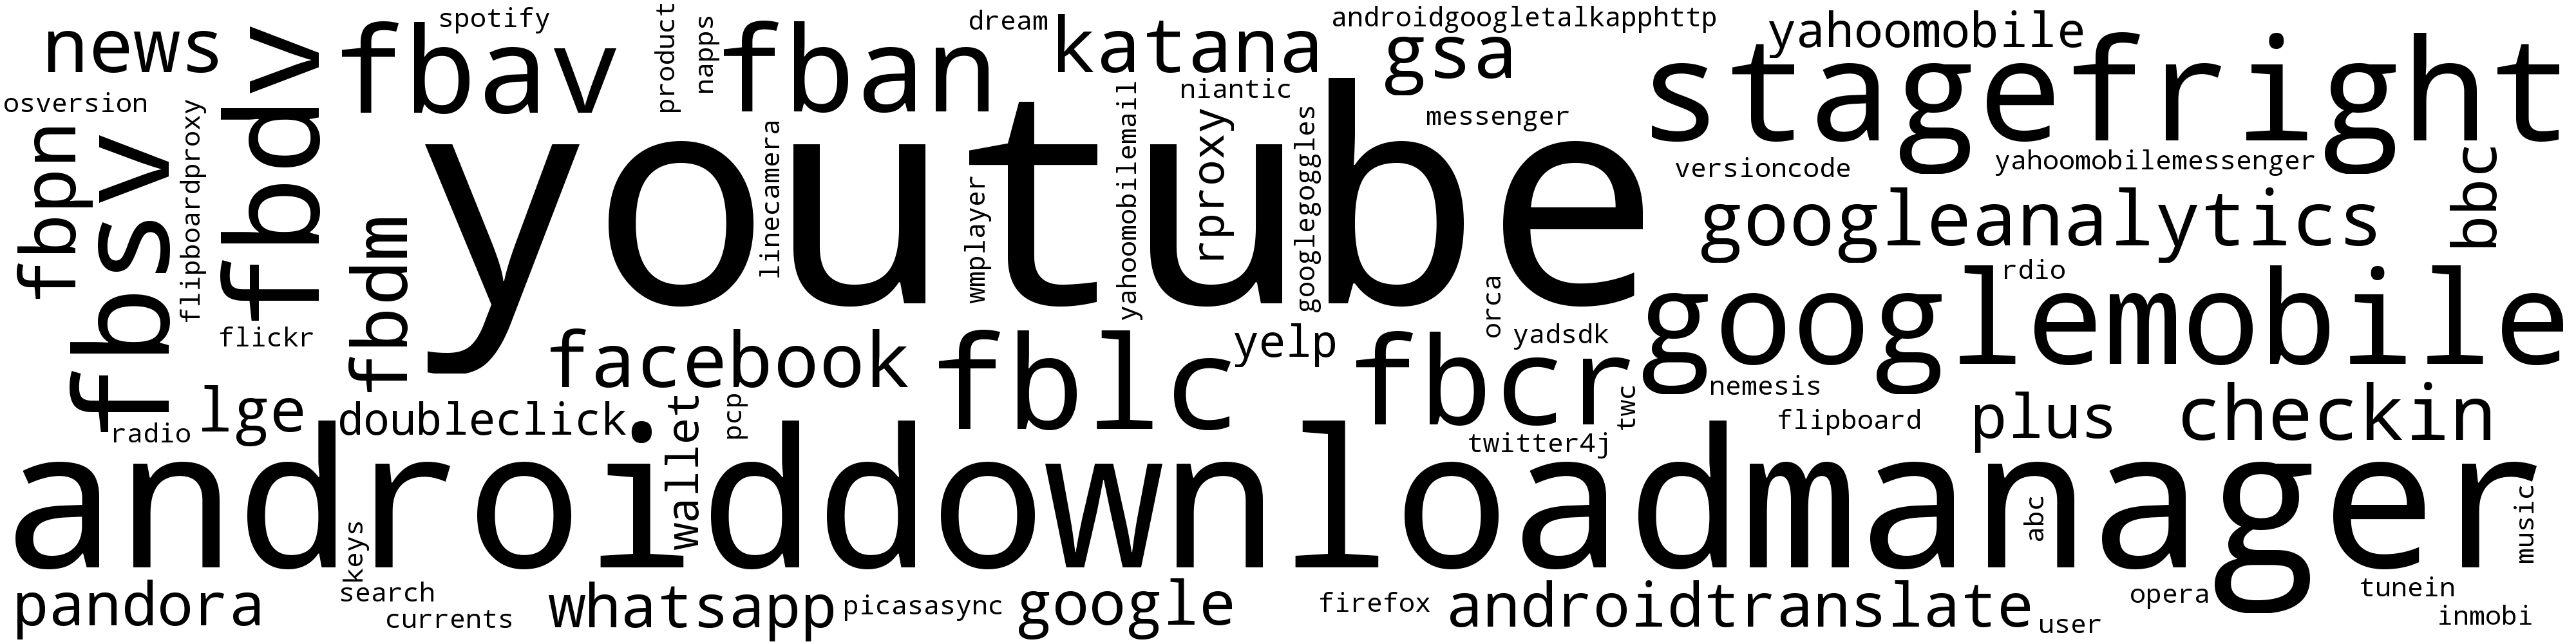
\includegraphics[width=\columnwidth]{figures/wordcloud_useragentsignature_android_image.png}}
\caption{\textbf{\useragent signatures in  iOS and Android HTTP flows.} \emph{The font weight represents the number of users for which a particular signature was observed.}}
%\vspace{\postfigspace}
\label{fig:http-wordcloud}
\end{figure}

%We now describe the results of classifying HTTP traffic in the \mobWild dataset. %mapping data gathered from our user study.
%Using only the \useragent on the \mobWild dataset, we were able to identify 256 iOS and 86 Android apps, OS libraries, and services. 
%The \emph{word cloud} in Fig.~\ref{fig:http-wordcloud} contains the summary of our results; the font size of an app/service name is proportional to the number of users for which it was observed.
%Note that \emph{Apple Core Media} and \emph{Stagefright} are services for downloading media content on iOS and Android devices, respectively.
%For the iOS devices in the \mobWild dataset, we observe a signature of \emph{Apple Core Media} in more than 98.45\% of the content downloaded from the YouTube servers (identified by their \httphost field).
%Similarly, we observe that YouTube flows contain ``Stagefright'' in HTTP headers. % to Android devices depending on the OS version. 
%We observe a similar signatures for other popular media services such as Netflix, YouTube, Vimeo, Pandora, etc, so we use the \httphost field to identify these Web services.
%\drc{AM: Suggests removing word cloud. PG doesn't like them either.}

\begin{table}
\centering
\begin{small}
\begin{tabular}{|p{0.15\columnwidth}|p{0.2\columnwidth}|c|c|c|c|}
\hline
\multirow{2}{*}{\bf Technique}&\multirow{2}{*}{\bf Category} & \multicolumn{2}{c|}{\bf iOS} &  \multicolumn{2}{c|}{\bf Android} \tabularnewline
\cline{3-6}
&   & {\bf Bytes}  & {\bf Flows} & {\bf Bytes} & {\bf Flows}   \tabularnewline
&   & {\bf (\%)}  & {\bf (\%)} & {\bf (\%)} & {\bf (\%)}   \tabularnewline

\hline
\multirow{2}{*}{\useragent} &Apps             & 43.21  & 85.73 & 15.01 & 75.17 \tabularnewline
\cline{2-6}
                            & OS Services$^{*}$            &  0.19  & 3.82 & 17.42 & 0.81 \tabularnewline
\hline
\useragent + &Media (Popular)         & 51.36  & 7.12  & 61.98 & 3.56 \tabularnewline
\cline{2-6}
\httphost  &Media (Other)           & 4.90  &  0.85 &  0.68 &  0.12 \tabularnewline
\hline
\httphost & Other Apps/Web-services  & $<$0.01 & 0.49 & 1.53  & 12.98 \tabularnewline
\hline
\multicolumn{2}{|c|}{Total Classified}  & {\bf 99.6} & {\bf 98.01} & {\bf 96.62} & {\bf 92.64} \tabularnewline
\hline
\end{tabular}
\end{small}
\caption{\textbf{Effectiveness of mapping HTTP traffic}. \emph{OS services$^{*}$ includes services other than those used to download media content.}}
\label{tab:classify-http}
\end{table}

\textbf{In situ data.}
Table~\ref{tab:classify-http} shows that a combination of \useragent and \httphost field in HTTP headers can map more than 92\% of the traffic (flows and bytes) from iOS and Android devices.

Using only the \useragent on the \mobWild dataset, we were able to identify 256 iOS and 86 Android apps, OS libraries, and services. 
We observe that the \useragent is more effective in identifying iOS apps compared to Android apps, which concurs with what we observed during our controlled experiments.

The \emph{word cloud} in Fig.~\ref{fig:http-wordcloud} contains the signatures we extracted from the \useragent; the font size of an app/service name is proportional to the number of users for which it was observed.
Signatures such as facebook and youtube are useful in identifying the apps, Facebook and YouTube respectively.
However, signatures such as applecoremedia and stagefright represent the OS services provided by iOS and Android to download media content which are internally used by media streaming apps such as Pandora and YouTube.
Audio and video streaming apps such as Pandora and YouTube use the \emph{Apple Core Media} and \emph{Stagefright} services on iOS and Android respectively to download media content, and for other auxiliary content such as list of related videos and recommendations these apps use the \useragent that contains their app signature.
We therefore use a combination of \useragent and \httphost field to identify such apps.

In Table~\ref{tab:classify-http}, we observe that media from popular streaming services---Netflix, YouTube, Pandora, Spotify, and Vimeo---contribute to more than 50\% of the traffic volume from iOS and Android devices in the \mobWild dataset.
We also observe that unmapped media served from CDNs and others hosts comprises less than 5\% of the traffic volume for the iOS and Android devices. 
We also observe that the \httphost field is more useful to classify Android traffic compared to iOS traffic, which concurs with what we observed during our controlled experiments. 

To summarize, by using a combination of \useragent and \httphost we were able to classify more than 92\% of the iOS and Android traffic by flows and bytes. 
%\drc{From PG: How is mapping to organization done?}

\subsubsection{SSL Traffic Mapping without Decryption}

SSL flows provide limited information in plaintext to identify apps. 
For the traces captured during our controlled experiments, we use SSL bumping to map HTTP flows using the techniques described in the previous section. 
However, we did not perform SSL bumping for the devices in the \mobWild dataset, so we now describe how to 
map SSL flows \emph{without decryption}. 

\noindent\textbf{Overview of mapping technique.}
Using port numbers, we observe in that more than 98\% of SSL flows observed in our controlled experiments were due to HTTPS, the rest of the flows were due to email, instant messaging, and OS notification services. 
We therefore focus our attention on identifying the apps responsible for the HTTPS flows.
We use DNS responses and subsequent SSL handshakes to determine the \emph{hostnames} of the remote hosts contacted by mobile devices.
After identifying the hostnames, we try to map these hostnames to apps using the technique described in the previous section.

%During manual examination of the results, we observe that Google and Apple to the be two main groups of organizations: Google and Apple.

% After identifying a hostname, we map the corresponding traffic in two phases.
% In the first phase we use the port number and hostname to identify the service 
% and group the traffic based on service. \drc{Why are you using the term ``service'' instead of app? 
% Why is this classification so different from the previous section? Need to make it more uniform.}
% The five most popular groups that we found in our dataset are social network, mail, media, instant messages, and notification.
% For example, flows to \url{facebook.com}, \url{twitter.com}, \url{plus.google.com} are grouped as social networks.
% Traffic to well known email ports such as TCP port 993, and traffic to hosts such as \url{mail.google.com} are classified as mail traffic.
% Similarly, we use documented ports to identify notification services (Android push) and instant messages (Facebook Messenger).

% In the second phase, we group hostnames that do not contain details of Web services.
% For example, the hostname \url{fbcdn-photos-a.akamaihd.net} indicates that the traffic is due to Facebook (due to \emph{fbcdn}), while \url{www.googleapis.com} hides the underlying app.
% We group hostnames that hide the app and Web service based on the parent organization.
% During manual examination of the traces, we observe two main groups: Google Services and Apple Services.
% Google Services includes flows whose remote hosts are served by Google, \eg \url{www.googleapis.com}, while Apple Services includes flows to servers managed by Apple, \eg \url{*.phobos.apple.com}
% This mapping, though crude, gives insights on the key sources of SSL traffic.

\noindent\textbf{Identifying hostname using the SSL Handshake.}
We first use the common name (CN) field of certificates to identify the servers that exchanged data using HTTPS.
We observe that less than 25\% of the HTTPS traffic from iOS and Android contains the fully qualified domain name (FQDN) in the subject of the certificate; the rest of the traffic either contains regular expressions such as *.google.com or is a continuation of a previous SSL session. 
To further resolve the hostnames, we rely on the \emph{Server Name Indication} (SNI) used by SSL flows~\cite{rfc:servernametls}.
Servers that host multiple services use the SNI to distinguish these services.   
For example, we observe an SNI of \url{plus.google.com} and \url{s.youtube.com} in two flows that used a certificate with a CN \url{*.google.com}.
Using either the certificate or the SNI we were able to identify the hostname for less than 40\% of HTTPS traffic.

\noindent\textbf{Identifying hostname using the DNS messages.} 
For the remaining flows we use DNS messages exchanged by the mobile device with its DNS server before starting the HTTPS flows, a technique similar to DN-Hunter~\cite{bermudez:dnhunter}.
DN-Hunter relies on the most recent FQDN that corresponds to the IP address, however in our controlled experiments we observe Android and iOS devices use the first entry in DNS response while resolving hostnames.
We therefore use the latest DNS response that contains the IP address of the Web service in the first position.
In spite of the potential usefulness of DNS responses, we give a high priority to the SNI and the certificates because the DNS response differs from these in 9.2\% of the iOS traffic and 5.6\% of Android traffic.
This difference is due to caching of DNS responses by the apps.

% \begin{table}
% \centering
% \begin{small}
% \begin{tabular}{|p{0.1\columnwidth}|p{0.2\columnwidth}|c|c|c|c|}
% \hline
% \multirow{2}{*}{\bf Phase} & \multirow{2}{*}{\bf Category} & \multicolumn{2}{c|}{\bf iOS Traffic} &  \multicolumn{2}{c|}{\bf Android Traffic} \tabularnewline
% \cline{3-6}
%  &         & {\bf Bytes}  & {\bf Flows} & {\bf Bytes} & {\bf Flows}   \tabularnewline
%  &         & {\bf (\%)}  & {\bf (\%)} & {\bf (\%)} & {\bf (\%)}   \tabularnewline
% \hline
% \multirow{5}{*}{Apps (A)}
% & Social Ntwks    & 12.81 &  7.74 & 35.39 & 19.28 \tabularnewline
% \cline{2-6}
% & Mail               &  6.11 &  9.26 &  6.46 & 11.02 \tabularnewline
% \cline{2-6}
% & Media              &  0.94 &  0.25 &  3.66 &  3.62 \tabularnewline
% \cline{2-6}
% & Instant Msg   &  3.70 & 14.09 &  0.21 &  0.48 \tabularnewline
% \cline{2-6}
% & Notifications     &  4.69 & 17.45 &  2.02 &  6.57 \tabularnewline
% \cline{2-6}
% %\hline
% & \emph{Total (A) }       & {\em 28.25} & {\em 48.79} & {\em 47.74} & {\em 40.97} \tabularnewline
% \hline
% \multirow{2}{*}{Organization (B)}
%  & Google Svcs   & 36.32 & 17.56 & 47.31 & 48.27 \tabularnewline
% \cline{2-6}
%  & Apple Svcs    & 25.26 & 28.26 & $<$0.01 & $<$0.01 \tabularnewline
% \cline{2-6}
% \cline{2-6}
% & \emph{Total (B) }       & {\em 61.58} & {\em 45.82} & {\em 47.31} & {\em 48.27} \tabularnewline
% \hline
% \multicolumn{2}{|c|}{\emph{Total (A + B)}}       & {\em \bf 89.83} & {\em\bf 94.61} & {\em\bf  96.10}  &  {\em\bf  89.24} \tabularnewline
% \hline
% \end{tabular}
% \end{small}
% \caption{\textbf{Mapping SSL traffic in the \mobWild dataset.} \emph{The iOS and Android SSL traffic in the \mobWild dataset is dominated by Google and Apple Services. The share of Social Network traffic is higher for Android devices because the default photo backup services on Android devices uses the Google Plus (and Picasa) Social Network.}}
% \label{tab:classify-ssl-traffic}
% \end{table}



\begin{table}
\centering
\begin{small}
\begin{tabular}{|p{0.3\columnwidth}|c|c|c|c|}
\hline
\multirow{2}{*}{\bf App/Org} & \multicolumn{2}{c|}{\bf iOS Traffic} &  \multicolumn{2}{c|}{\bf Android Traffic} \tabularnewline
\cline{2-5}
                              & {\bf Bytes}  & {\bf Flows} & {\bf Bytes} & {\bf Flows}   \tabularnewline
                              & {\bf (\%)}  & {\bf (\%)} & {\bf (\%)} & {\bf (\%)}   \tabularnewline
\hline

Apps            & 28.25 & 48.79 & 47.74 & 40.97 \tabularnewline
\hline
Google Services & 36.32 & 17.56 & 47.31 & 48.27 \tabularnewline
\hline
Apple Services  & 25.26 & 28.26 & $<$0.01 & $<$0.01 \tabularnewline
\hline
{\emph{Total}}  & {\em \bf 89.83} & {\em\bf 94.61} & {\em\bf  96.10}  &  {\em\bf  89.24} \tabularnewline
\hline
\end{tabular}
\end{small}
\caption{\textbf{Mapping SSL traffic in the \mobWild dataset.} \emph{The SSL traffic from the iOS and Android devices in the \mobWild dataset is dominated by Google and Apple services.}}
\label{tab:classify-ssl-traffic}
\end{table}

\noindent\textbf{Mapping results.} 
Table~\ref{tab:classify-ssl-traffic} shows our SSL mapping results on the SSL traffic in the \mobWild dataset. 
We first group hostnames to the apps and we were able to identify the apps for more than 40\% of the iOS and Android SSL flows.
For flows whose hostnames are ambiguous, we group them according to organizations.
During manual examination of the results, we observe that Google and Apple to be the two main organizations that contributed to the majority of the flows; we label these flows as Google Services and Apple services respectively. 

In Table~\ref{tab:classify-ssl-traffic}, we observe that 61.5\% of iOS and 47.3\% of Android traffic (by bytes) is respectively 
to Google and Apple servers where the hostname does not contain signatures of the app.
This share does not include the traffic to Google and Apple servers that we classified as apps.
For example, flows to \url{mail.google.com} were classified as GMail and are placed in the category apps, while flows to \url{www.googleapis.com} is categorized as Google Services. 
Google services and Apple services are therefore the largest sources of SSL traffic in our \mobWild dataset.

In summary, using the certificates, SNI, and DNS messages, we were able to identify the hostname of the remote hosts for more than 89\% of the SSL flows.
We observe that Google and Apple are the dominant sources of SSL traffic for the Android and iOS devices in the \mobWild dataset.

\subsubsection{Summary}

We use the a combination of \useragent and \httphost field to identify apps responsible for HTTP flows.
On applying our technique to the \mobWild dataset, we were able to classify more than 92\% of the iOS and Android traffic by flows and bytes. 
We observe that the \useragent field is more effective to identify HTTP flows from iOS devices compared to Android devices.
We speculate that this behavior is because of the strict coding practices mandated by Apple while packaging iOS apps~\cite{xcode:distrib}.

We use certificates, SNI, and DNS messages to map SSL flows, and we were able to classify more than 90\% of SSL traffic in the \mobWild dataset using our classification technique. 
To the best of our knowledge, we are the first to study the effectiveness of these fields in classifying SSL flows from mobile devices.

%%% Local Variables: 
%%% mode: latex
%%% TeX-master: "main"
%%% End: 




\section{Classification Methodology}
\label{sec:classification-methodology}

\platname offers a network perspective of the mobile Internet traffic.
To detail the mobile traffic, we need to first identify the access technology used by the devices, and the applications and Web-services responsible for each flow captured by \platname.
In this section we describe the technique we used to identify the access technology and the applications and Web-services. 

\subsection{Access Technology Classification}

To quantify the impact of the access technology, we need to first identify the access technology used by the devices when accessing the Internet via \platname servers.
A mobile devices can access the Internet using either \wifi or cellular networks. 
We estimate the access technology with the description of the AS through which the mobile client connects to our \platname server. 
We get this AS description by performing a \emph{WHOIS} lookup on the IP address used by the mobile client to tunnel Internet traffic. 
For our analysis, we use the WHOIS databases available at \emph{whois.cmyru.com} and \emph{utrace.de}.
We use the information from these \emph{WHOIS} databases to manually classify the ASes to be either cellular or \wifi.
Our dataset consists of data traffic from 54 distinct ASes, of which we classify 9 to belong to cellular networks.
Each device connected our \platname server from at most two distinct ASes during the measurement study.
In contrast, a median of 4 \wifi ASes were observed per device and for one device we observed traffic from 25 different \wifi ASes that were spread across 5 countries. 

\subsection{Classification of Mobile Applications and Services}

The data traffic from mobile devices is because of the applications running on the device and OS services and libraries used by the applications. 
To analyze the behavior of mobile services we need to first associate the observed flows with the applications and the OS services responsible for the flows.
For our analysis, we focus on identifying the OS services and the applications and Web-services responsible for HTTP and SSL flows, the largest sources of mobile Internet traffic~\cite{maier:mobtraffic,falaki:mobileusage,xu:appusage}.

\begin{table}
\begin{small}
\begin{center}
\begin{tabular}{|p{0.15\columnwidth}|p{0.12\columnwidth}|r|r|r|r|}
\hline
\multirow{2}{*}{\bf IP Protocol} & \multirow{2}{*}{\bf Service} & \multicolumn{2}{|c|}{\bf Android} & \multicolumn{2}{|c|}{\bf iOS} \tabularnewline
\cline{3-6}
           &           &  \textbf{Cell.}  &  \textbf{\wifi}  &  \textbf{Cell.}  &  \textbf{\wifi}  \tabularnewline
\hline
\multirow{3}{*}{TCP}
       &  HTTP  & 35.386 & 68.686 & 52.109 & 75.506 \tabularnewline
\cline{2-6}
       &  SSL   & 61.135 & 27.366 & 46.765 & 18.777 \tabularnewline
\cline{2-6}
       &  other & 2.346  & 3.290  & 0.256  & 1.818 \tabularnewline
\hline
\multirow{2}{*}{UDP}
       &  DNS   & 0.682  & 0.496  & 0.545  & 0.305  \tabularnewline
\cline{2-6}
       &  other & 0.316  & 0.098  & 0.286  & 3.583  \tabularnewline
\hline
 Other &  -     & 0.135  & 0.064 & 0.039  & 0.011  \tabularnewline
\hline
\multicolumn{2}{|c|}{\emph{total}} & 100.00 & 100.00 & 100.00 & 100.00 \tabularnewline
\hline
\end{tabular}
\end{center}
\end{small}
\caption{Traffic volume (in percentage) of popular protocols and services on Android and iOS devices over cellular and \wifi.
\emph{TCP flows are responsible for more than 90\% of traffic volume. Traffic share of SSL over cellular networks is more than twice the traffic share of SSL over \wifi.}} 
\label{tab:summaryIOSAndroidTraffic}
\end{table}

We begin our identification process using the classification provided Bro~\cite{bro}.
Bro uses the protocol field in the IP header to broadly classify the flows, and we use this classification to label flows as either TCP, UDP, or \emph{other}.
Bro further classifies TCP flows using well defined port numbers, and we use this classification to label flows as either HTTP, SSL (which includes HTTPS, IMAP, etc.) or \emph{other} flows.
Similarly, we use Bro to label UDP flows as either DNS or \emph{other}. 
Indeed, in \fref{tab:summaryIOSAndroidTraffic}, we observe that more than 92\% of the traffic in our \mobWild dataset is either HTTP or SSL. 
We also observe that the share of HTTP volume over \wifi and ce
llular are significantly different. 
This increase is a result of the reduced share of media traffic and the use of email and for social networking applications that rely on SSL.

\subsubsection{HTTP Traffic Classification}

Differences with ~\cite{erman2011http,xu:appusage,maier:mobtraffic}.

Web-services rely on the \useragent field to distinguish HTTP flows from their mobile applications from the flows originating from Web-browsers.
In our controlled experiments we observed a valid \useragent string in more than 99\% of the HTTP flows from Android and iOS.
However, because the mobile applications use built in OS services and libraries to download media content, we do not observe the identifier of the application using the OS service and library in the \useragent string for media traffic. 
For example, when an iOS devices is used to stream YouTube video on a YouTube Application or if the video is viewed on clicking a video link on Facebook application, we observe that the media content is downloaded by AppleCoreMedia service of iOS~\cite{apple:coremedia}. 
We now show how a combination of \useragent and \httphost can be used to identify either the Web-service or the application associated with the flow.

\begin{figure}
\subfloat[iOS]{\label{fig:http-wordcloud-ios}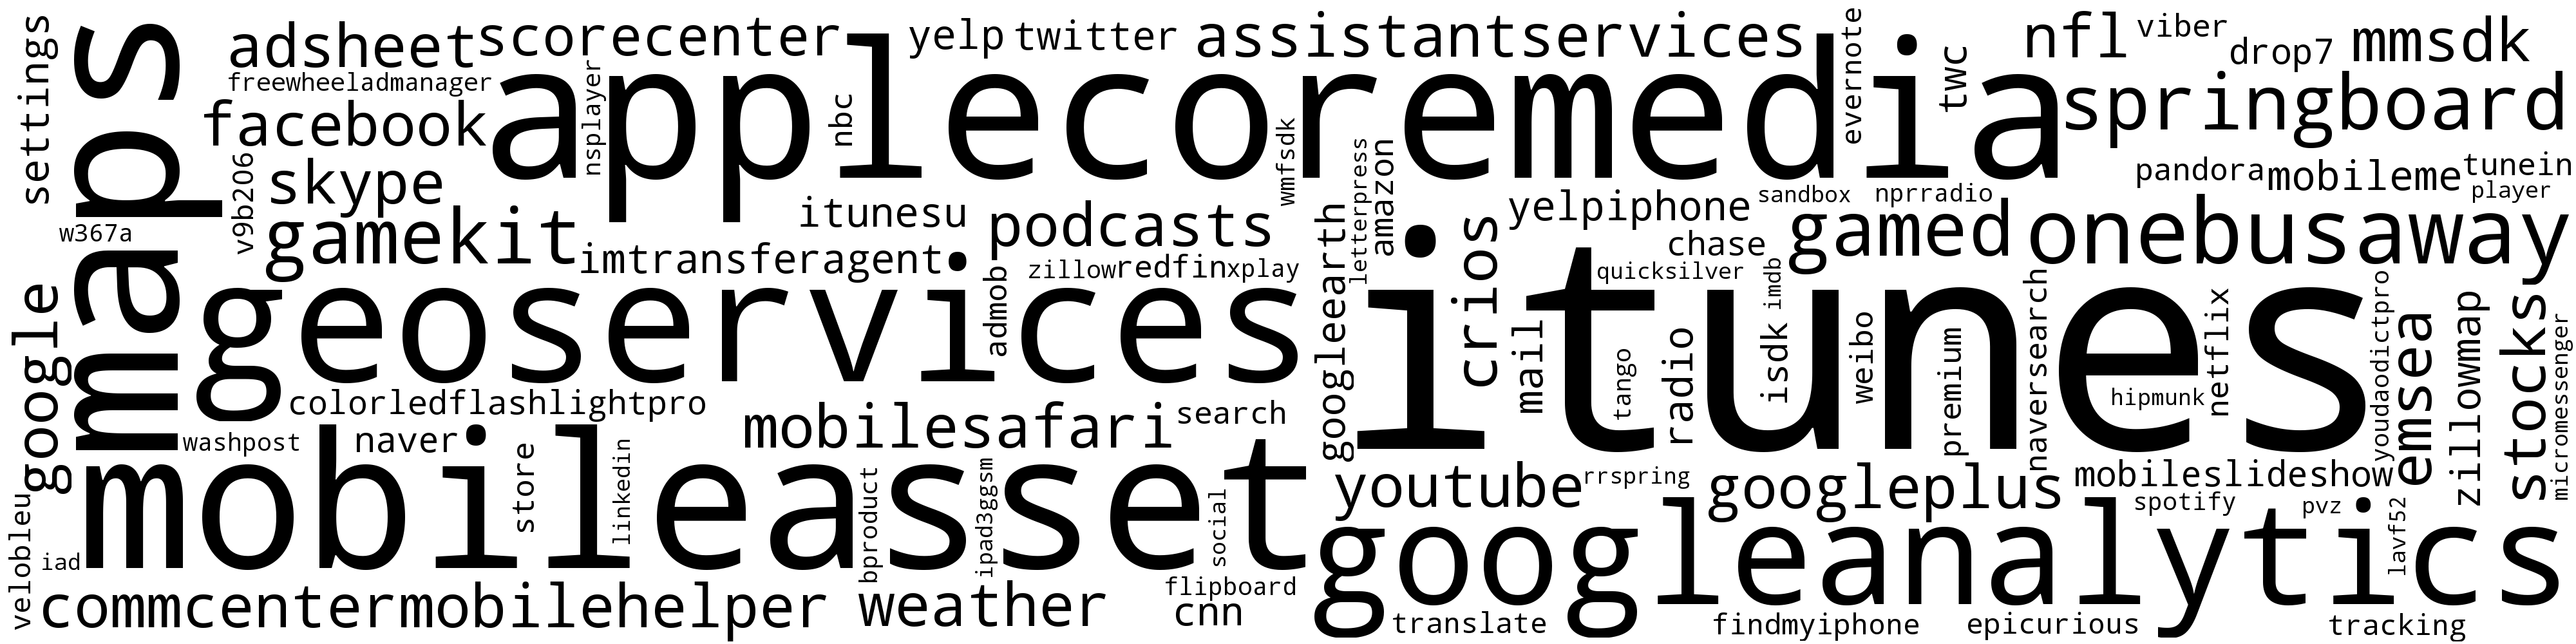
\includegraphics[width=\columnwidth]{figures/wordcloud_useragentsignature_ios_image.png}}\newline
\subfloat[Android]{\label{fig:http-wordcloud-android}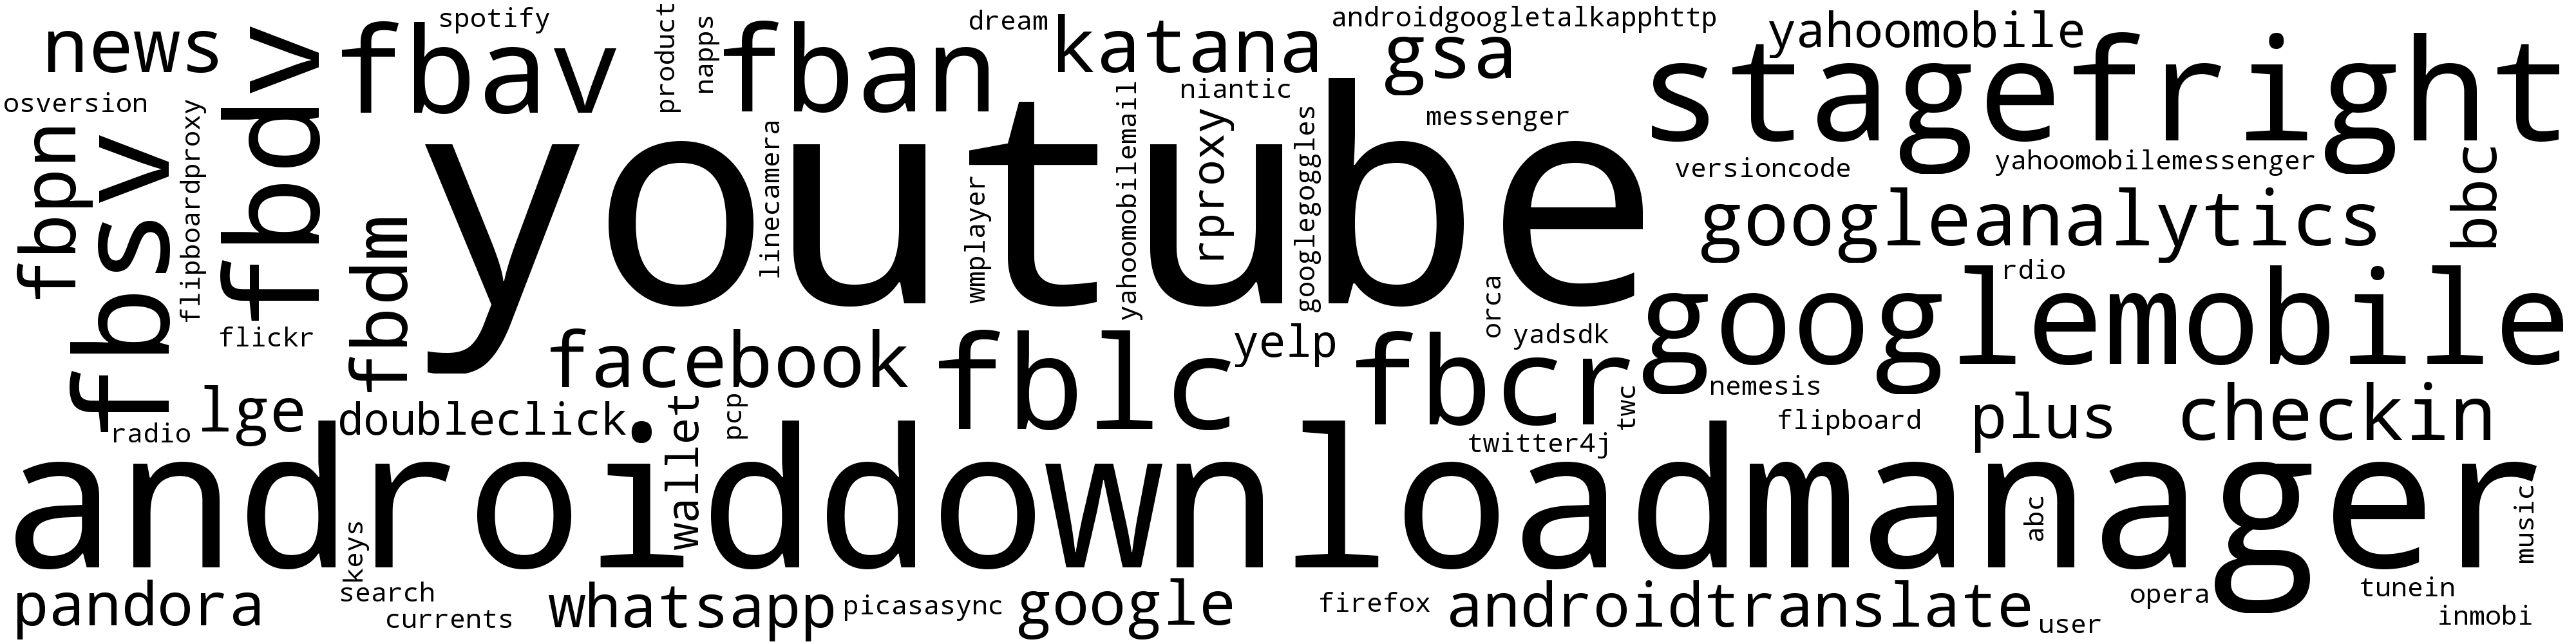
\includegraphics[width=\columnwidth]{figures/wordcloud_useragentsignature_android_image.png}}
\caption{\useragent signatures in  iOS and Android HTTP flows. \emph{The font weight represents the number of users for which a particular signature was observed.}}
\label{fig:http-wordcloud}
\end{figure}

We observe that more than 98\% of HTTP traffic from Android and iOS devices in the \mobWild dataset have a valid \useragent string; we observe a total of 1435 unique \useragent strings across Android and iOS devices. 
These \useragent strings contain an application identifier and other auxiliary information such as details of the OS, manufacturer, display resolutions, carrier, and information such as versions and compatibility with other browser engines~\cite{mozilla:useragentdetection}. 
We use regular expression to extract the tokens that contain the application information, and cluster these tokens using edit distance\footnote{We plan to release this code along with \platname package.}.
At the end of this process we were able to identify 361 unique signatures which we resolve as either applications or OS services. 

In \fref{fig:http-wordcloud} we present a \emph{word cloud} of the signatures we were able to extract from \useragent field; the text size of the signature represents the number of users for which the signature was observed.
Despite the usefulness of the \useragent, we observe that relying only on the \useragent is not sufficient to identify the application.
For example, we observe the signatures \emph{applecoremedia} and \emph{stagefright} in the \emph{word cloud} for iOS devices and Android devices, signatures of the OS services responsible to download media content.

The iOS devices rely on AppleCoreMedia service~\cite{apple:coremedia} to download media content.
We therefore observed the signature of AppleCoreMedia in more than 98.45\% of the content downloaded from the YouTube servers (which we identify based on the \httphost field in the \httpget requests). 
Similarly, depending the Android version we observe either the signature for Stagefright\cite{android:stagefright} or no application or OS service signature for YouTube traffic to Android devices. 
Indeed, we observed signatures for popular media services such as Netflix, YouTube, Vimeo, Pandora, etc. in the \httphost field in the majority traffic from iOS devices and Android devices. 
We therefore used the \httphost field to classify media content.

\begin{table}
\centering
\begin{small}
\begin{tabular}{|p{0.25\columnwidth}|c|c|c|c|}
\hline
\multirow{2}{*}{\bf Category} & \multicolumn{2}{c|}{\bf iOS} &  \multicolumn{2}{c|}{\bf Android} \tabularnewline
\cline{2-5}
  & {\bf Bytes}  & {\bf Flows} & {\bf Bytes} & {\bf Flows}   \tabularnewline
\hline
Media (Popular)         & 51.405  & 12.131 & 65.922 & 22.377 \tabularnewline
\hline
Application             & 33.987  & 80.758 & 31.353 & 77.498 \tabularnewline
\hline
Media (Other)       & 14.572  &  5.914 &  2.712 &  0.044 \tabularnewline
\hline
Other                   &  0.036  & 1.1963 &  0.013 &  0.081 \tabularnewline
\hline
{\em total}            & 100 & 100 & 100 & 100 \tabularnewline
\hline
\end{tabular}
\end{small}
\caption{Classification of HTTP Traffic.}
\label{tab:classify-http}
\end{table}

In summary, we use a combination of \useragent and \httphost field in HTTP headers to classify HTTP traffic.
In \fref{tab:classify-http}, a table that provides an overview of our classification results.
We observe that we were able to classify more than 98\% of the traffic in terms of flows and bytes from iOS and Android devices using the \useragent and the \httphost field. 
We observe that media from popular hosts contribute to more than 50\% of the traffic volume from iOS and Android devices.
Similarly, we were able to identify applications for more than 77\% of flows from Android and iOS devices. 
However, we observe media (identified based on the \useragent) served from CDNs and others hosts from which we could not identify the webservice from other fields in the HTTP header and the DNS responses before the HTTP flows to be 14.5\% of the traffic volume for the iOS devices in our dataset.

\subsubsection{Classification of SSL Traffic.}

Unlike HTTP flows, SSL flows provide limited information that can be used to identify the applications. 
Our objective classifying SSL traffic was therefore focused towards identifying the Web-services responsible for the SSL flows. 
We now show how we used the port number, the SSL certificate with server name identification, and DNS queries to identify the source of SSL traffic. 

\begin{table}
\centering
\begin{small}
\begin{tabular}{|p{0.25\columnwidth}|c|c|c|c|}
\hline
\multirow{2}{*}{\bf Service} & \multicolumn{2}{c|}{\bf iOS} &  \multicolumn{2}{c|}{\bf Android} \tabularnewline
\cline{2-5}
  & {\bf Bytes}  & {\bf Flows} & {\bf Bytes} & {\bf Flows} \tabularnewline
\hline
HTTPS                   & 91.287 & 81.960 & 97.852 & 97.168    \tabularnewline
\hline
Mail                    &  6.700 & 15.872 & 0.689  & 0.320  \tabularnewline
\hline
Notification            &  1.412 & 1.553  & 1.321  & 2.100  \tabularnewline
\hline
Other                   &  0.601 & 0.615  & 0.138  & 0.412 \tabularnewline
\hline
{\em total}             & 100 & 100 & 100 & 100 \tabularnewline
\hline
\end{tabular}
\end{small}
\caption{Classification of SSL Traffic based on port number. \emph{HTTPs is the most popular service that uses SSL in the \mobWild dataset.}}
\label{tab:classify-ssl-port}
\end{table}

Mobile devices use SSL for various services including mail, notifications, instant messaging, and web browsing.
Services such as mail, instant messaging, and notifications are documented to use dedicated port numbers of their traffic\footnote{We also use the AS for identifying the notification messages as detailed in \fref{sec:characterize-os}.}
On using port numbers, we observe in \fref{tab:classify-ssl-port} that a majority of SSL traffic by volume and flows is HTTPS.
We then focus our attention on indentifying the Web-services responsible for the HTTPs flows. 

We first use the common name (CN) field of certificates to identify the servers that exchanged data using HTTPS.
We observe that less than 25\% of the HTTPS traffic from iOS and Android contains the fully qualified domain name (FQDN) in the subject of the certificate; the rest of the traffic either contains regular expressions such as *.google.com in the certificate or is a continuation of a previous SSL session. 
To further resolve the hostnames, we rely on \emph{server name indication} used by SSL flows~\cite{rfc:servernametls}.
Servers that host multiple services use the \emph{server name indication} to distinguish these services.   
For example, we observe a \emph{server name indication} of \emph{plus.google.com} and \emph{s.youtube.com} in two flows that used a certificate with a CN \emph{*.google.com}.
However, we observe that by using either the certificate or the \emph{server name} we were able to identify the name of the Web-service in less than \tbd{40}\% of iOS and Android HTTPS traffic.

For such flows we use DNS requests made by the mobile devices before starting the HTTPS flows, a technique similar to DN-Hunter~\cite{bermudez:dnhunter}.
DN-Hunter relies on the most recent FQDN that corresponds to the IP address, however in our controlled experiments we observe Android and iOS devices use the first entry in DNS response while resolving \emph{hostnames}.
We therefore use the latest DNS response that contains the IP address of the webservice in the first position of the DNS response. 
Indeed, for 97.8\% of the Android and 83.4\% of the iOS HTTPS traffic that we could not classify using other fields, we observe that the latest DNS response before the flow started contained the IP address of the webservice as the first entry in the DNS response\footnote{The share of SSL traffic where the latest DNS response contains the IP address of the web-service in the first position is 97.4\% for Android and 88.6\% of iOS}. 
Despite the potential usefulness of DNS responses, we give a high priority to the server-name and the certificates because we observed that for flows that contained the server name did not contain the same name in the DNS response for 9.2\% of the iOS traffic and 5.6\% of Android traffic.

\begin{table}
\centering
\begin{small}
\begin{tabular}{|c|c|}
\hline
{\bf iOS} & {\bf Android} \tabularnewline
\hline
imap.gmail.com & picasaweb.google.com \tabularnewline
www.google.com & www.googleapis.com \tabularnewline
sphotos-a.xx.fbcdn.net & android.clients.google.com \tabularnewline
itunes.apple.com  & clients4.google.com \tabularnewline
m.google.com & fbcdn-photos-a.akamaihd.net \tabularnewline
\hline
\end{tabular}
\end{small}
\caption{Popular hostnames for iOS and Android based on traffic volume.}
\label{tab:sslclassify-popular-host}
\end{table}

In \fref{tab:sslclassify-popular-host} we present the top5 hostnames that were responsible for 66\% of iOS traffic and 54\% of Android by volume. 
We observe that despite the hostname we cannot uniquely identify the application. 
For example, \emph{www.google-apis.com} and \emph{clients4.google.com} offer limited information on the application or web-service that is responsible for the content; one can only guess that these flows belong to some google service.
However, hostname such as \emph{fbcdn-photos-a.akamaihd.net} gives an indication that the traffic is due to facebook.

\begin{table}
\centering
\begin{small}
\begin{tabular}{|p{0.35\columnwidth}|c|c|c|c|}
\hline
\multirow{2}{*}{\bf Service} & \multicolumn{2}{c|}{\bf iOS} &  \multicolumn{2}{c|}{\bf Android} \tabularnewline
\cline{2-5}
  & {\bf Bytes}  & {\bf Flows} & {\bf Bytes} & {\bf Flows} \tabularnewline
\hline
Mail                 & 9.970    & 62.168   & 1.626  & 1.565 \tabularnewline
\hline
Social Networking    & 12.491   & 6.683    & 36.661 & 22.352 \tabularnewline
\hline
Apple/Google Store   & 5.457    & 3.463    & 0.044  & 0.036 \tabularnewline
\hline
Instant Messages     & 0.982    & 7.089    & 1.411  & 3.109 \tabularnewline
\hline
Other Google Services & 58.665   & 13.32510 & 45.024 & 46.089 \tabularnewline
\hline
\emph{total}         & 87.564   & 92.728   & 84.776 & 73.151 \tabularnewline
\hline
\end{tabular} 
\end{small}
\caption{Sample classification of SSL traffic based on names in certificate, server name identification, and DNS request.}
\label{tab:classify-ssl-traffic}
\end{table}

In \fref{tab:classify-ssl-traffic} we show how we grouped SSL traffic based on names identified using the SSL fields and DNS queries and port numbers.
We observe that the iOS devices in our dataset generated a significant number of flows to email sites.
Similarly, we were able to group 12.49\% of iOS and 36.661\% of Android traffic with social network services that includes \emph{Google Plus, Facebook, and Twitter}.
We speculate the increase in traffic share for Android devices is because Android devices offer services to backup photos on \emph{Google Plus}.
Similarly, we observe that 5.4\% of the traffic from iOS devices was from Apple stores while we observe only 0.04\% of traffic to the \emph{Google Play} store. 
This low share is because google can use hosts matching the pattern \emph{client*.google.com} to serve for different Web-services.
We observed a similar behavior in our controlled experiments, and we group such traffic as \emph{other google services}.
Indeed, in \fref{tab:classify-ssl-traffic} we observe that traffic from Google is the largest source of SSL traffic for iOS and Android devices in our dataset. 

In summary, we use \platname to perform controlled experiments and in the wild measurements to characterize mobile Internet traffic. 
We use Bro to analyze the data and build on the output of bro to further classify HTTP flows and SSL flows to identify the source of the traffic. 
We now present the results of our experiments and measurements study. 


%%% Local Variables: 
%%% mode: latex
%%% TeX-master: "main.tex"
%%% End: 

% Popular webservices such as google are known to use the same pool of IP addresses for various applications, for example the IP for gmail may also be used for search. 
% In \fref{fig:ssl-classification-app-service} we present the fraction of SSL traffic where the most recent DNS response contained the IP address of the SSL flow in the first position. 
% We observe that for the majority of SSL traffic by volume and flows can be classified by using the DNS responses. 

% \begin{table}
% \centering
% \begin{small}
% \begin{tabular}{|p{0.35\columnwidth}|c|c|c|c|}
% \hline
% \multirow{2}{*}{\bf Service} & \multicolumn{2}{c|}{\bf iOS} &  \multicolumn{2}{c|}{\bf Android} \tabularnewline
% \cline{2-5}
%   & {\bf Bytes}  & {\bf Flows} & {\bf Bytes} & {\bf Flows} \tabularnewline
% \hline
% FQDN in Certificate    & 24.274 & 31.423  & 19.318 & 29.424 \tabularnewline
% \hline
% Regular expression     & 50.463 & 35.318  & 42.427 & 31.670 \tabularnewline
% \hline
% No Subject or CN       & 25.263 & 33.259  & 38.254 & 38.906 \tabularnewline
% \hline
% {\em total}            & 100 & 100 & 100 & 100 \tabularnewline
% \hline
% \end{tabular}
% \end{small}
% \caption{Classification of HTTPs based on certificates.}
% \label{tab:classify-http-cert}
% \end{table}

%\section{Network Characteristics of Notification Services}
\label{sec:characterize-os}

Mobile operating systems provide OS level notification services to optimize network usage.
The Apple Push Notification service (APNs) and Google Cloud Messaging (GCM)~\cite{gcm} are used by iOS and Android applications respectively to receive notifications from the Internet.
In this section we show how \platname was used to compare the notification services of iOS and Android, and detailing it behavior in the wild. 

\begin{figure}
\centering
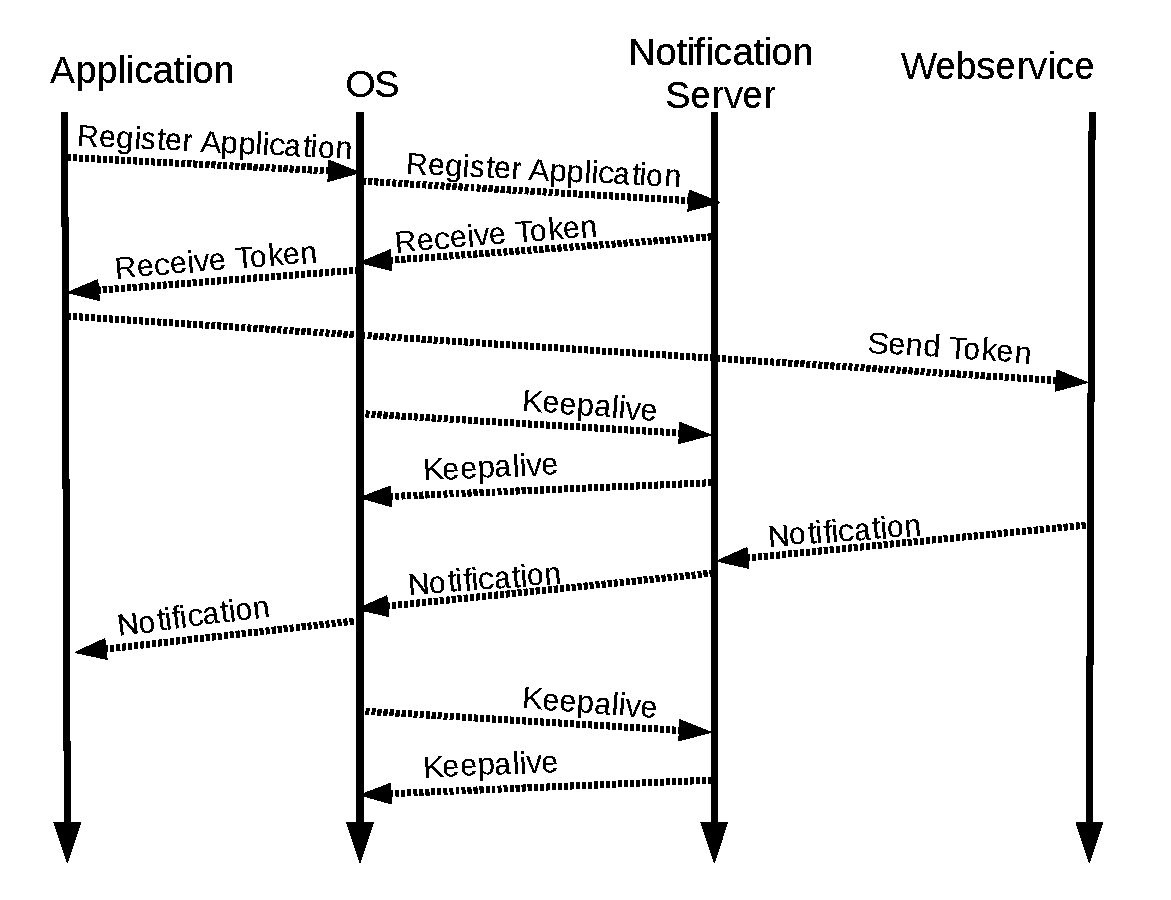
\includegraphics[width=\columnwidth]{figures/Notification.pdf}
\caption{Notifications on mobile OSes. \emph{Because notification messages are sent over TCP, keepalive messages are periodically exchanged to ensure TCP connections do not timeout.}}
\label{fig:push-expt-interarrival}
\end{figure}



\subsection{Controlled Experiment on Factory Reset Devices}

We first detail the detail the behavior of notification services by performing a controlled experiment on \emph{factory-reset} devices. 
The objective of this experiment was to analyze notification services for devices that are used \emph{out of the box}, and detail the impact of device manufacturer, and pre-installed applications. 

For our experiment, we performed a \emph{factory reset} on an iPod Touch, an iPad, an iPhone, a Samsung Galaxy SIII, and a Google Nexus S Phone; the reset was performed after their batteries were fully charged. 
We then perform the initialization step and assigned a dummy email account as the primary account to each of these devices.
We then allowed these devices to connect to the Internet over \wifi through \platname and monitored the Internet traffic from these devices.
We then studied the impact of access technology by letting the iPhone and Samsung Galaxy SIII tunnel traffic through \platname using cellular networks. 

We observed that the traffic volume during the 24 hour periods varied from 19~KB to 97~KB depending on the devices. 
We classify APNS and GCM messages using the TCP port numbers mentioned in their specifications~\cite{gcm, apns}.
Because we did not run any applications in the foreground, notification messages were responsible for largest fraction of the traffic volume; the share was 35\% for Nexus S, 88\% for the Samsung SIII and around 50\% for each of the iOS devices. 
The share of DNS traffic varied from 10\% to 40\% for each of the devices while the other services contributed to less than 10\% of the traffic volume.
The only exception was the Samsumg Galaxy SIII which used location services that contributed to 26\% of 47~KB traffic volume generated by the device.

\begin{figure}
\centering
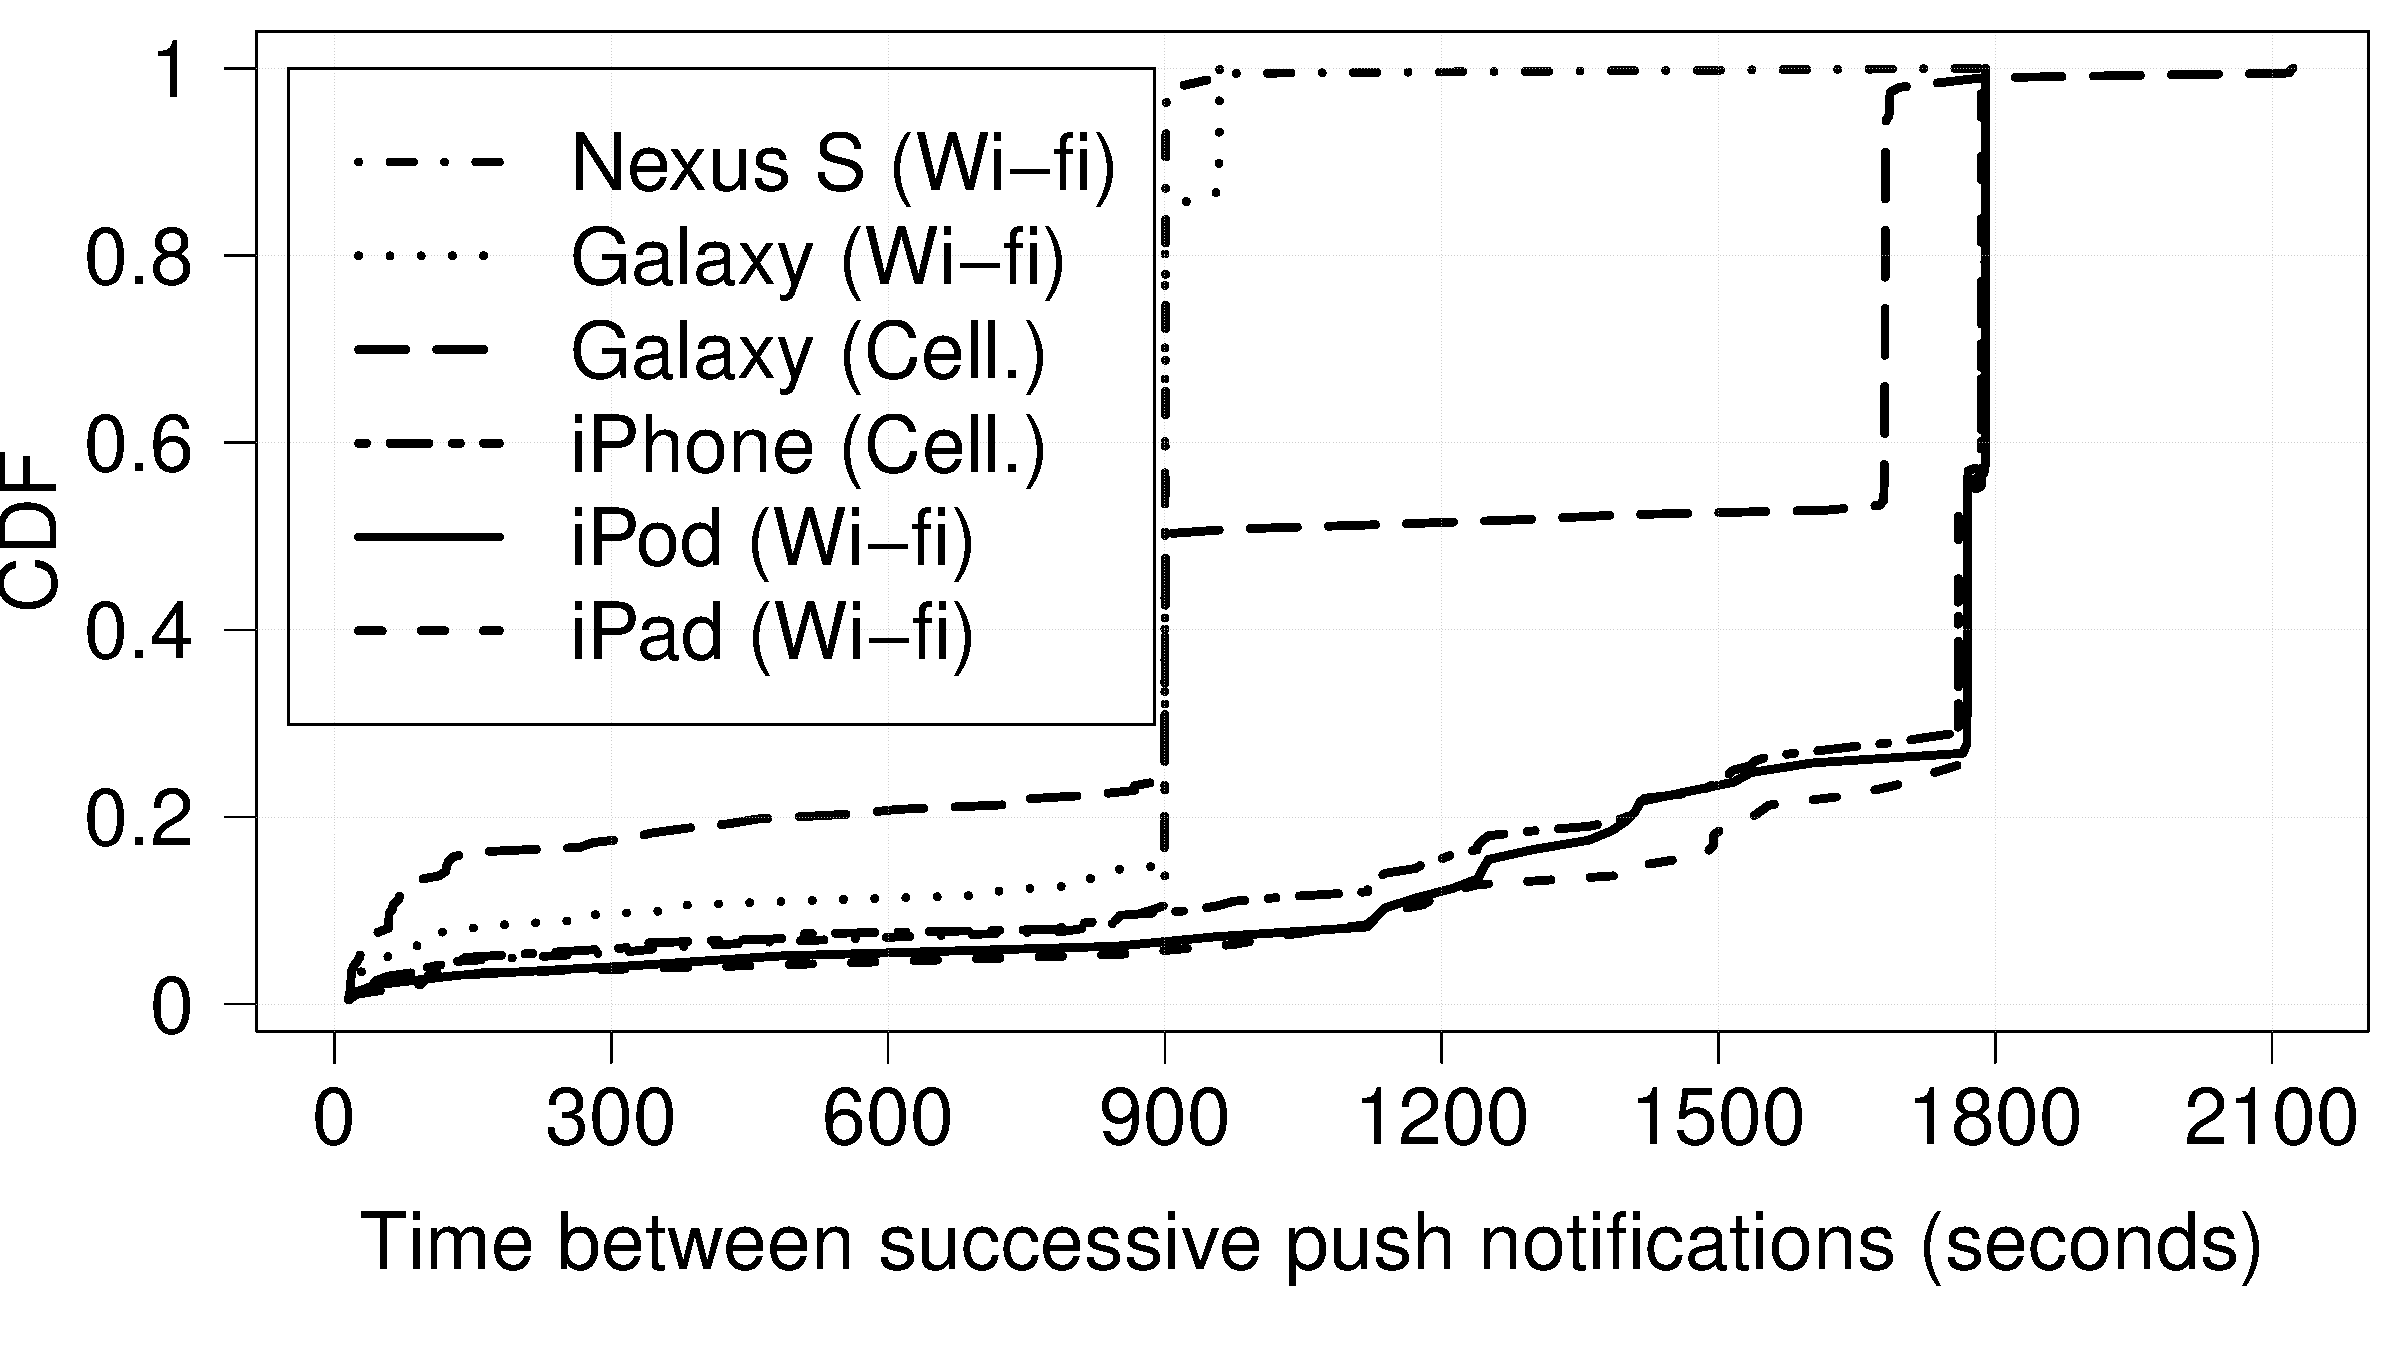
\includegraphics[width=\columnwidth]{plots/push_factoryreset_interarrival_distrib.pdf}
\caption{Inter-arrival time between notification messages after factory reset. \emph{The Android and iOS devices communicate with the notification server approximately once every 900~seconds and 1800 seconds respectively. The behavior of Android devices depends on the device, the pre-installed applications, and the access technology.}}
\label{fig:push-expt-interarrival}
\end{figure}

In \fref{fig:push-expt-interarrival} plot the time between successive messages sent by the notification servers on the ports assigned for notifications. 
We observe that the inter-arrival time between notifications for the Android devices is at least 900 seconds for more than 80\% of the notifications observed. 
The distribution of the inter-arrival time also depends on the access technology for the Samsung Galaxy SIII phone; we observe steps in the distribution for the SIII phone while we do not observe these steps when the same phone uses \wifi. 
We do not observe this difference when the Nexus S phone used the cellular data connection; we do not present the figure due to lack of space. 
\tbd{AR: Why these difference -- which applications stop coming up and so on}.
For the iOS devices, we observe an inter-arrival time at least 1700~seconds for that more than 75\% of the notifications in \fref{fig:push-expt-interarrival}. 
We do not observe a significant difference between the inter-arrival times for the iPhone over cell and \wifi and we do not present these results due to lack of space. 

On analyzing the packets exchanged, we observe that  all Android flows with an inter-arrival time larger than 800 seconds consisted of an empty TCP packet sent by the device followed by a 25 byte payload sent by the server.
Similarly, all iOS flows with an inter-arrival time larger than 1500 seconds began with an TCP packet with a payload of 85 bytes sent by the device followed by the server responding with of a TCP packet of 37 byte payload.

In summary, we observe notifications consume very little data, less than 50~KB in 24 hours, on Android and iOS devices in their default state.
The large time between successive notifications and the small amount of data exchanged implies they consume very little power.
We also observe that iOS devices have a larger time between successive notifications compared to Android devices in the default state. 
Furthermore, the inter-arrival time between notifications for Android devices differs based on the device manufacturer and the access technology. 

\subsection{Notifications In The Wild} 

We now characterize our observations on the notifications we observed in the \mobWild dataset. 
The objective of this analysis was to detail the frequency, traffic volume, and source of the notification services. 

\begin{figure}
\centering
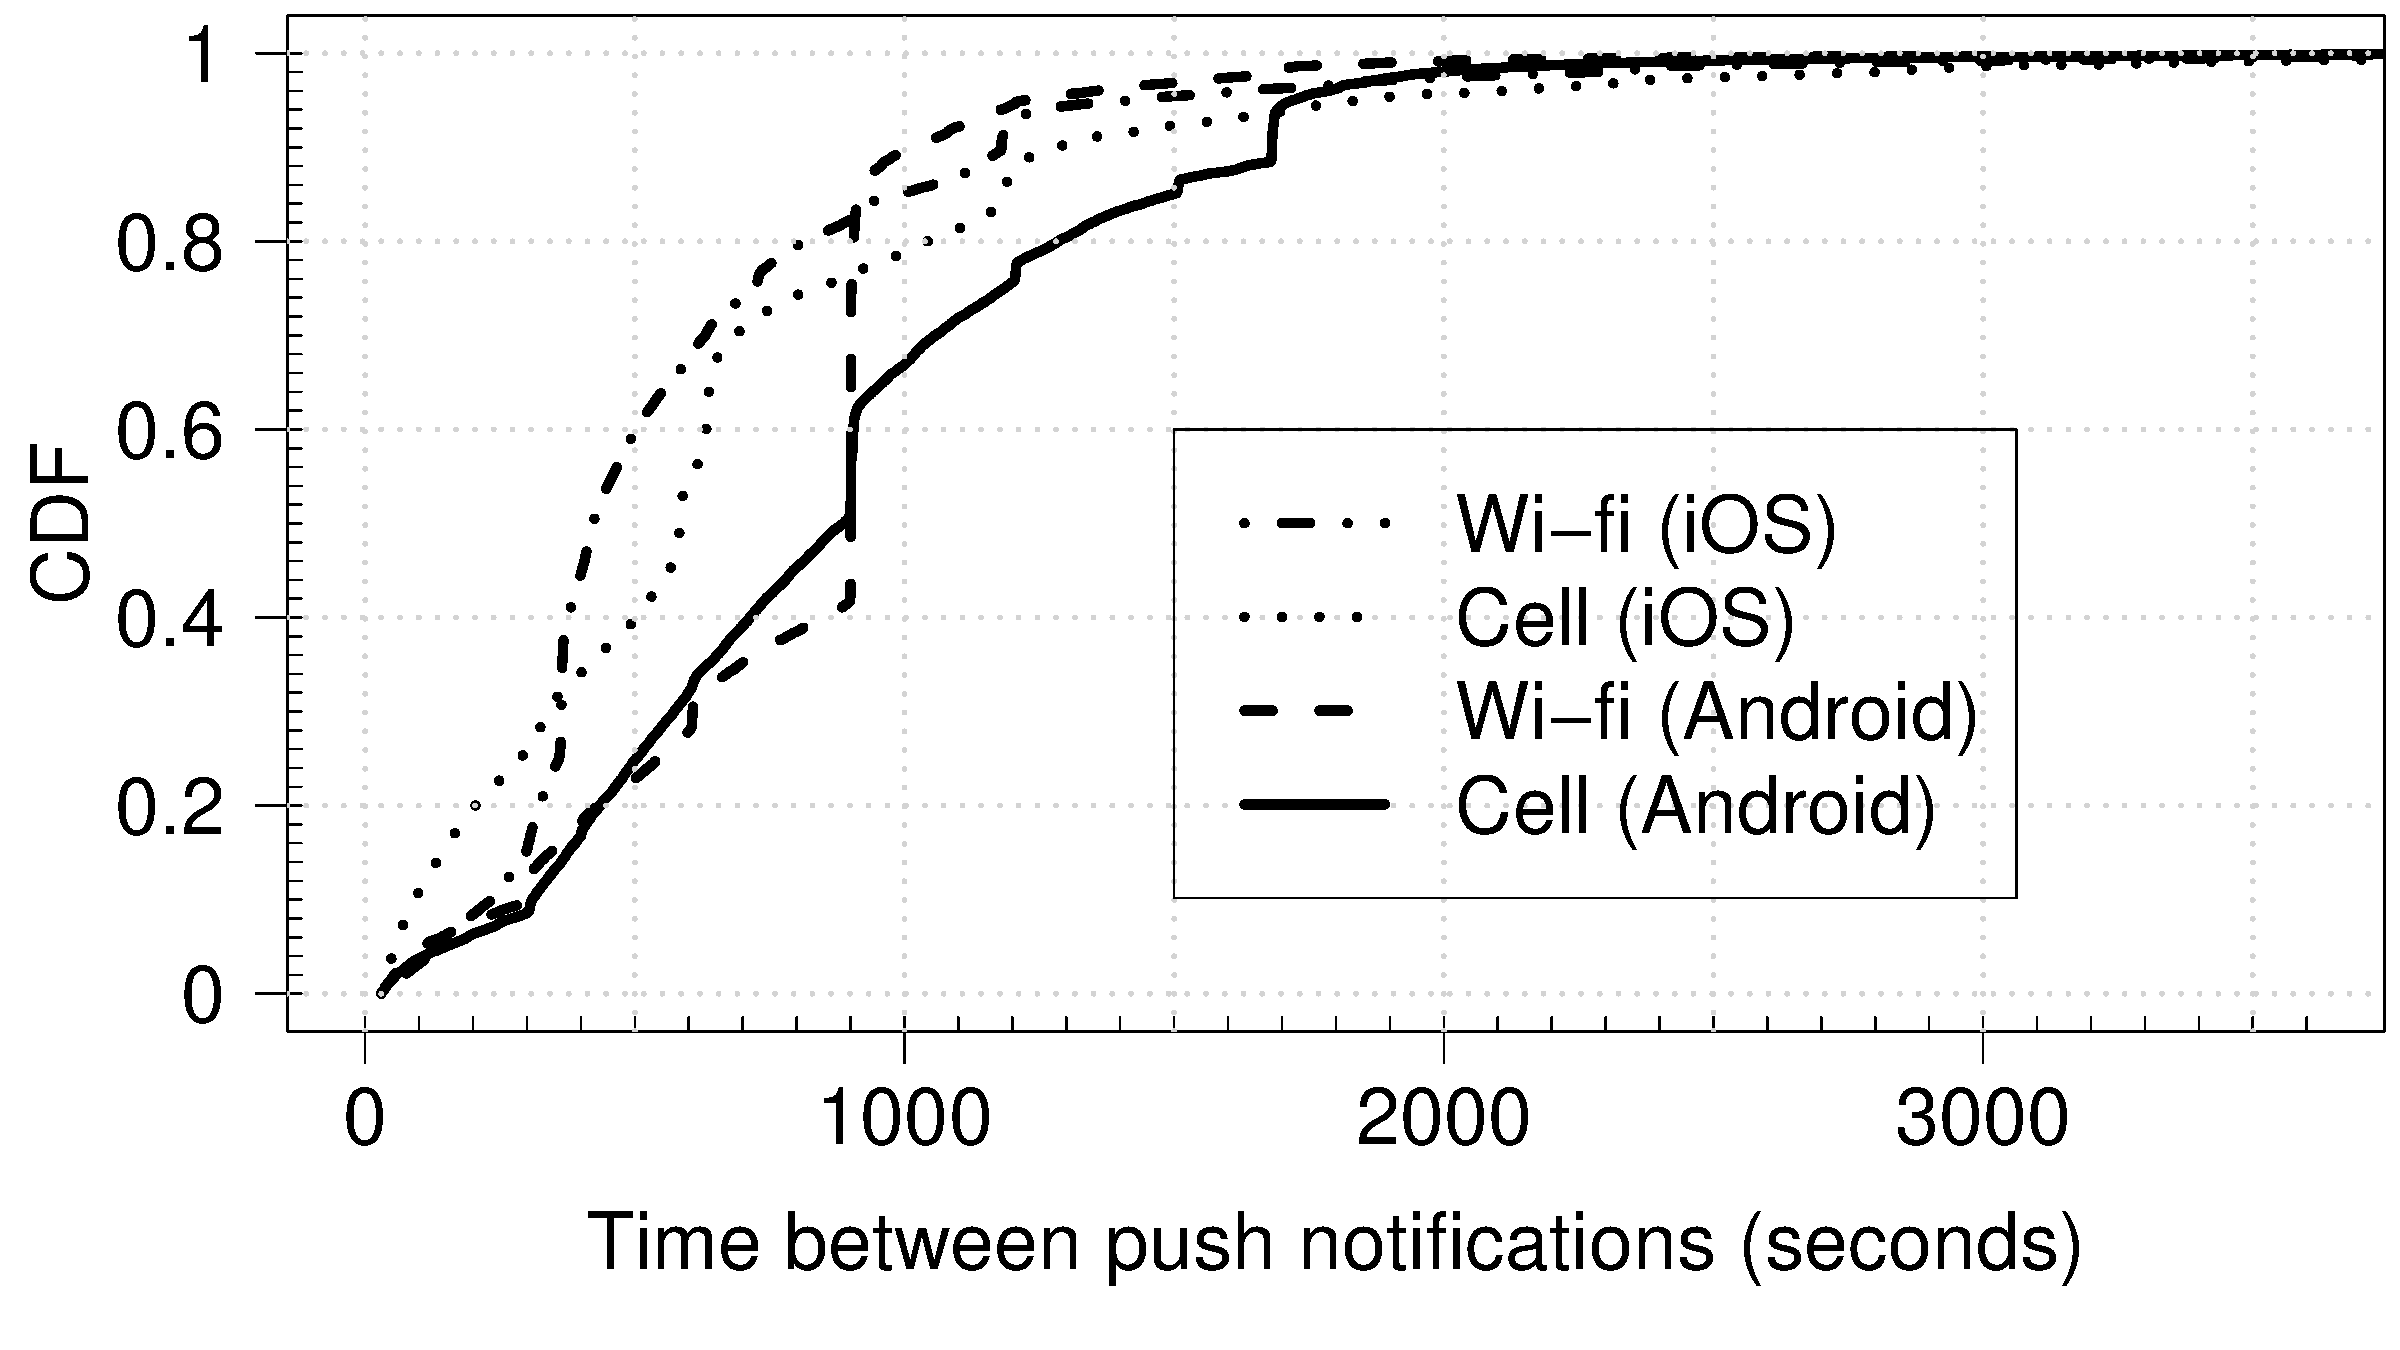
\includegraphics[width=\columnwidth]{plots/push_compare_os_tech_wild_distrib.pdf}
\caption{Distribution of the time between push notification messages in the wild. \emph{The frequency of push notification messages is higher for the iOS devices in our dataset compared to the Android devices. Notification messages are less frequent over cellular networks compared to Wi-Fi networks.}}
\label{fig:push-wild-compare-ostech}
\end{figure}

%The advantage of \platname is that it allows for direct comparison between devices across and their behavior across access technologies. 
To analyze the frequency of notification messages, we plot the distribution of the time between successive push notification messages for Android and iOS devices over cellular and \wifi networks in \fref{fig:push-wild-compare-ostech}.
In \fref{fig:push-wild-compare-ostech} we observe that a higher time between push notifications over cellular networks in comparison to \wifi networks for iOS and Android devices.  
We also observe the Android devices in our dataset receive notifications less frequently compared to the iOS devices in our dataset. 
We also observe a heavy tail for the time between notification messages which implies potentially long idle intervals.
\tbd{Correlation between time between notification messages and size of the next idle time observed?}


\begin{figure}
\centering
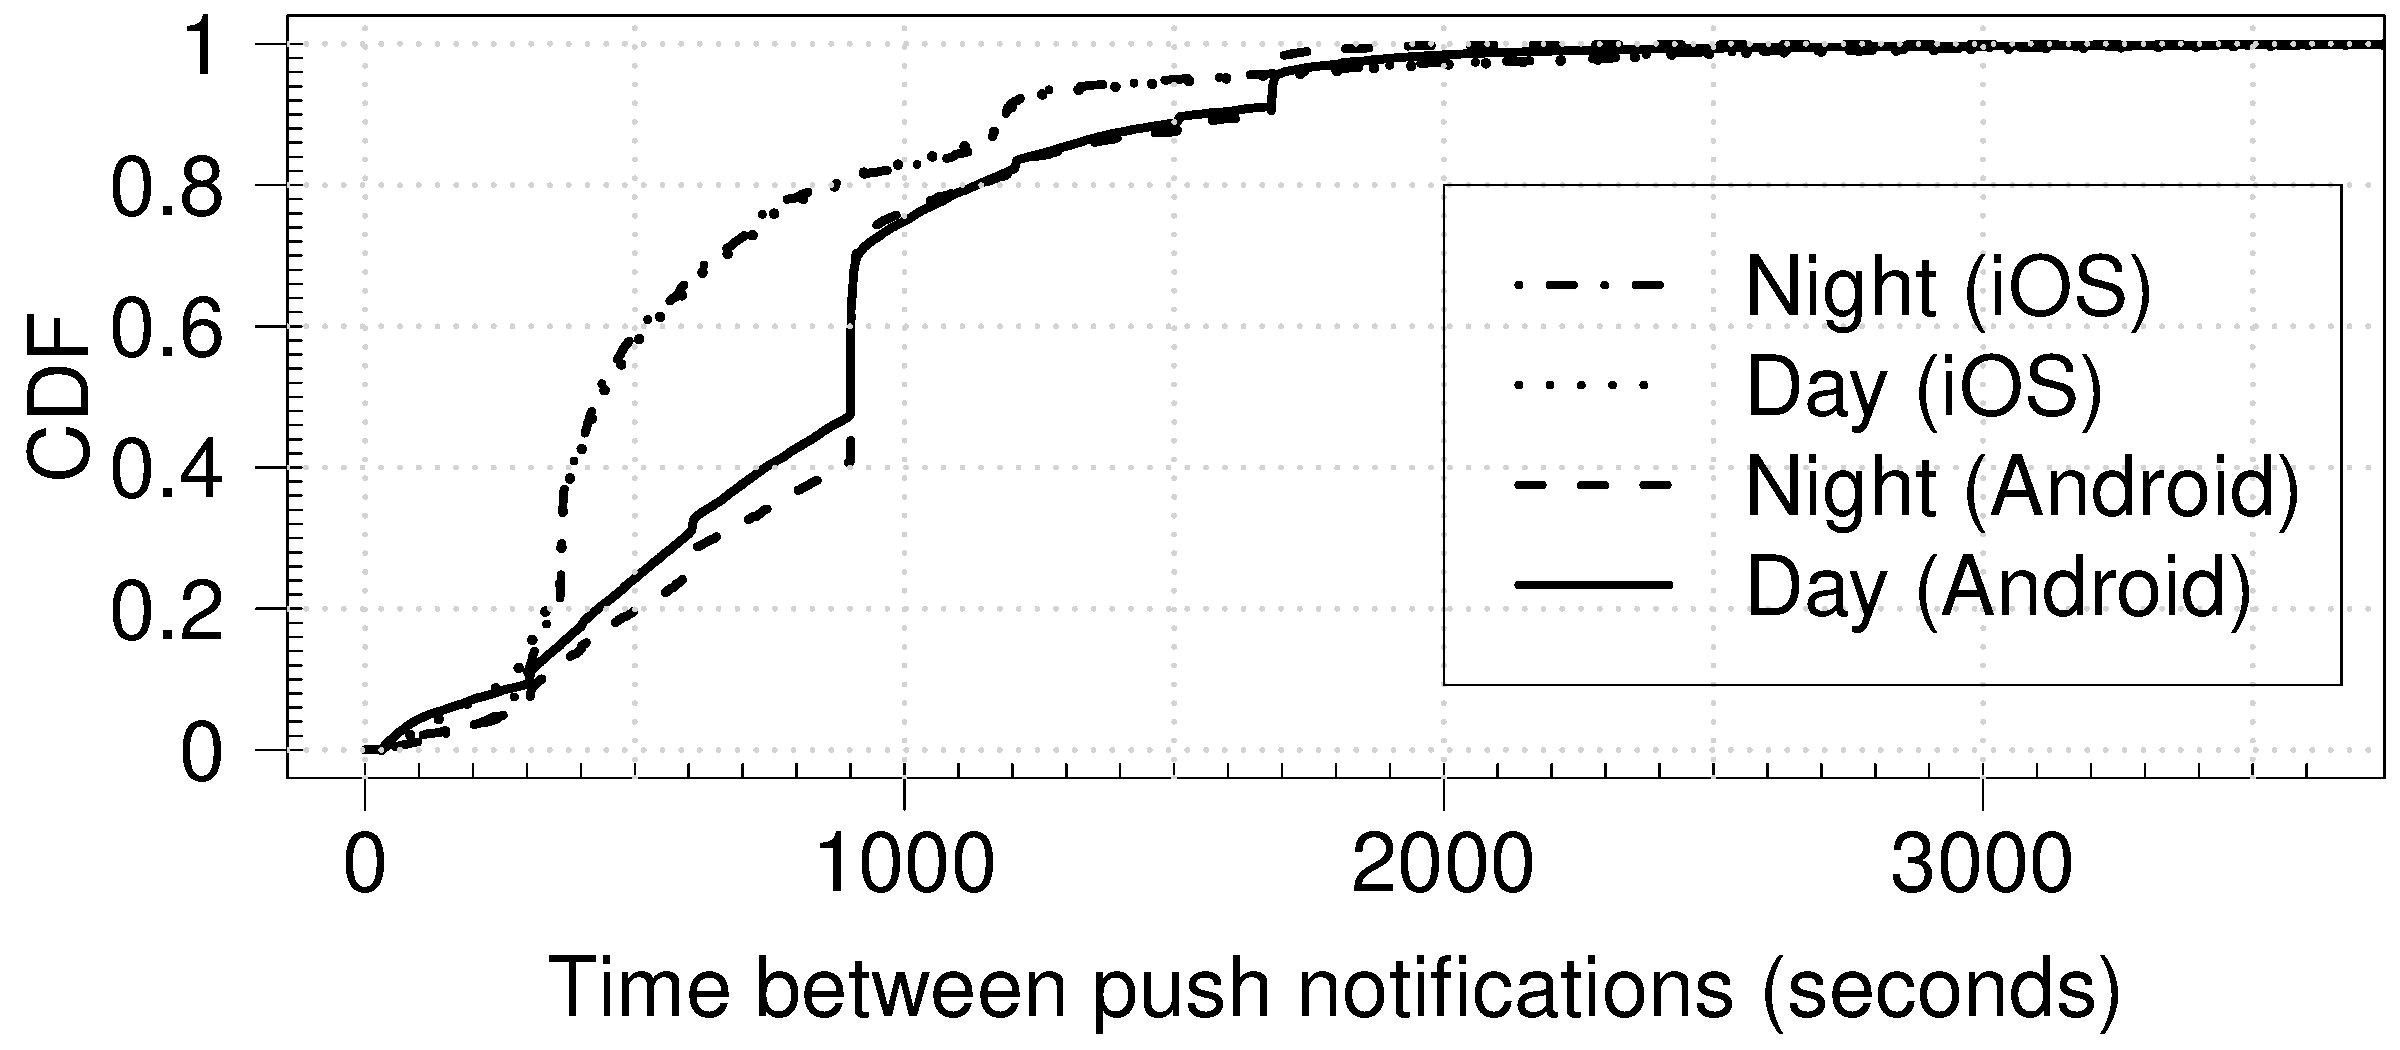
\includegraphics[width=\columnwidth]{plots/push_compare_diurnal_wild_distrib.pdf}
\caption{Impact of time-of-day on the push notifications. \emph{The rate of notifications is agnostic of the time of the day for iOS and Android devices.}}
\label{fig:push-wild-diurnal}
\end{figure}

The notification messages could be in response to user actions, for example, a mail server might receive a notification of a new message.
To analyze this impact, we notification messages received during two time intervals: from midnight to 6 am (night), and from 6 am to midnight (day). 
In \fref{fig:push-wild-diurnal}, we plot the distribution between successive notification messages for these two intervals. 
We observe that the Android and iOS devices appear to be agnostic of the time of the day. 
The iOS devices (from verion 6.0) come with a feature called \emph{Do Not Disturb (DND)} that does raise notification alarms on receiving notifications during specific time periods. 
We observe notification messages were received by the device that had enabled this feature during the intervals their users had configured as \emph{Do Not Disturb}.

\begin{figure}
\centering
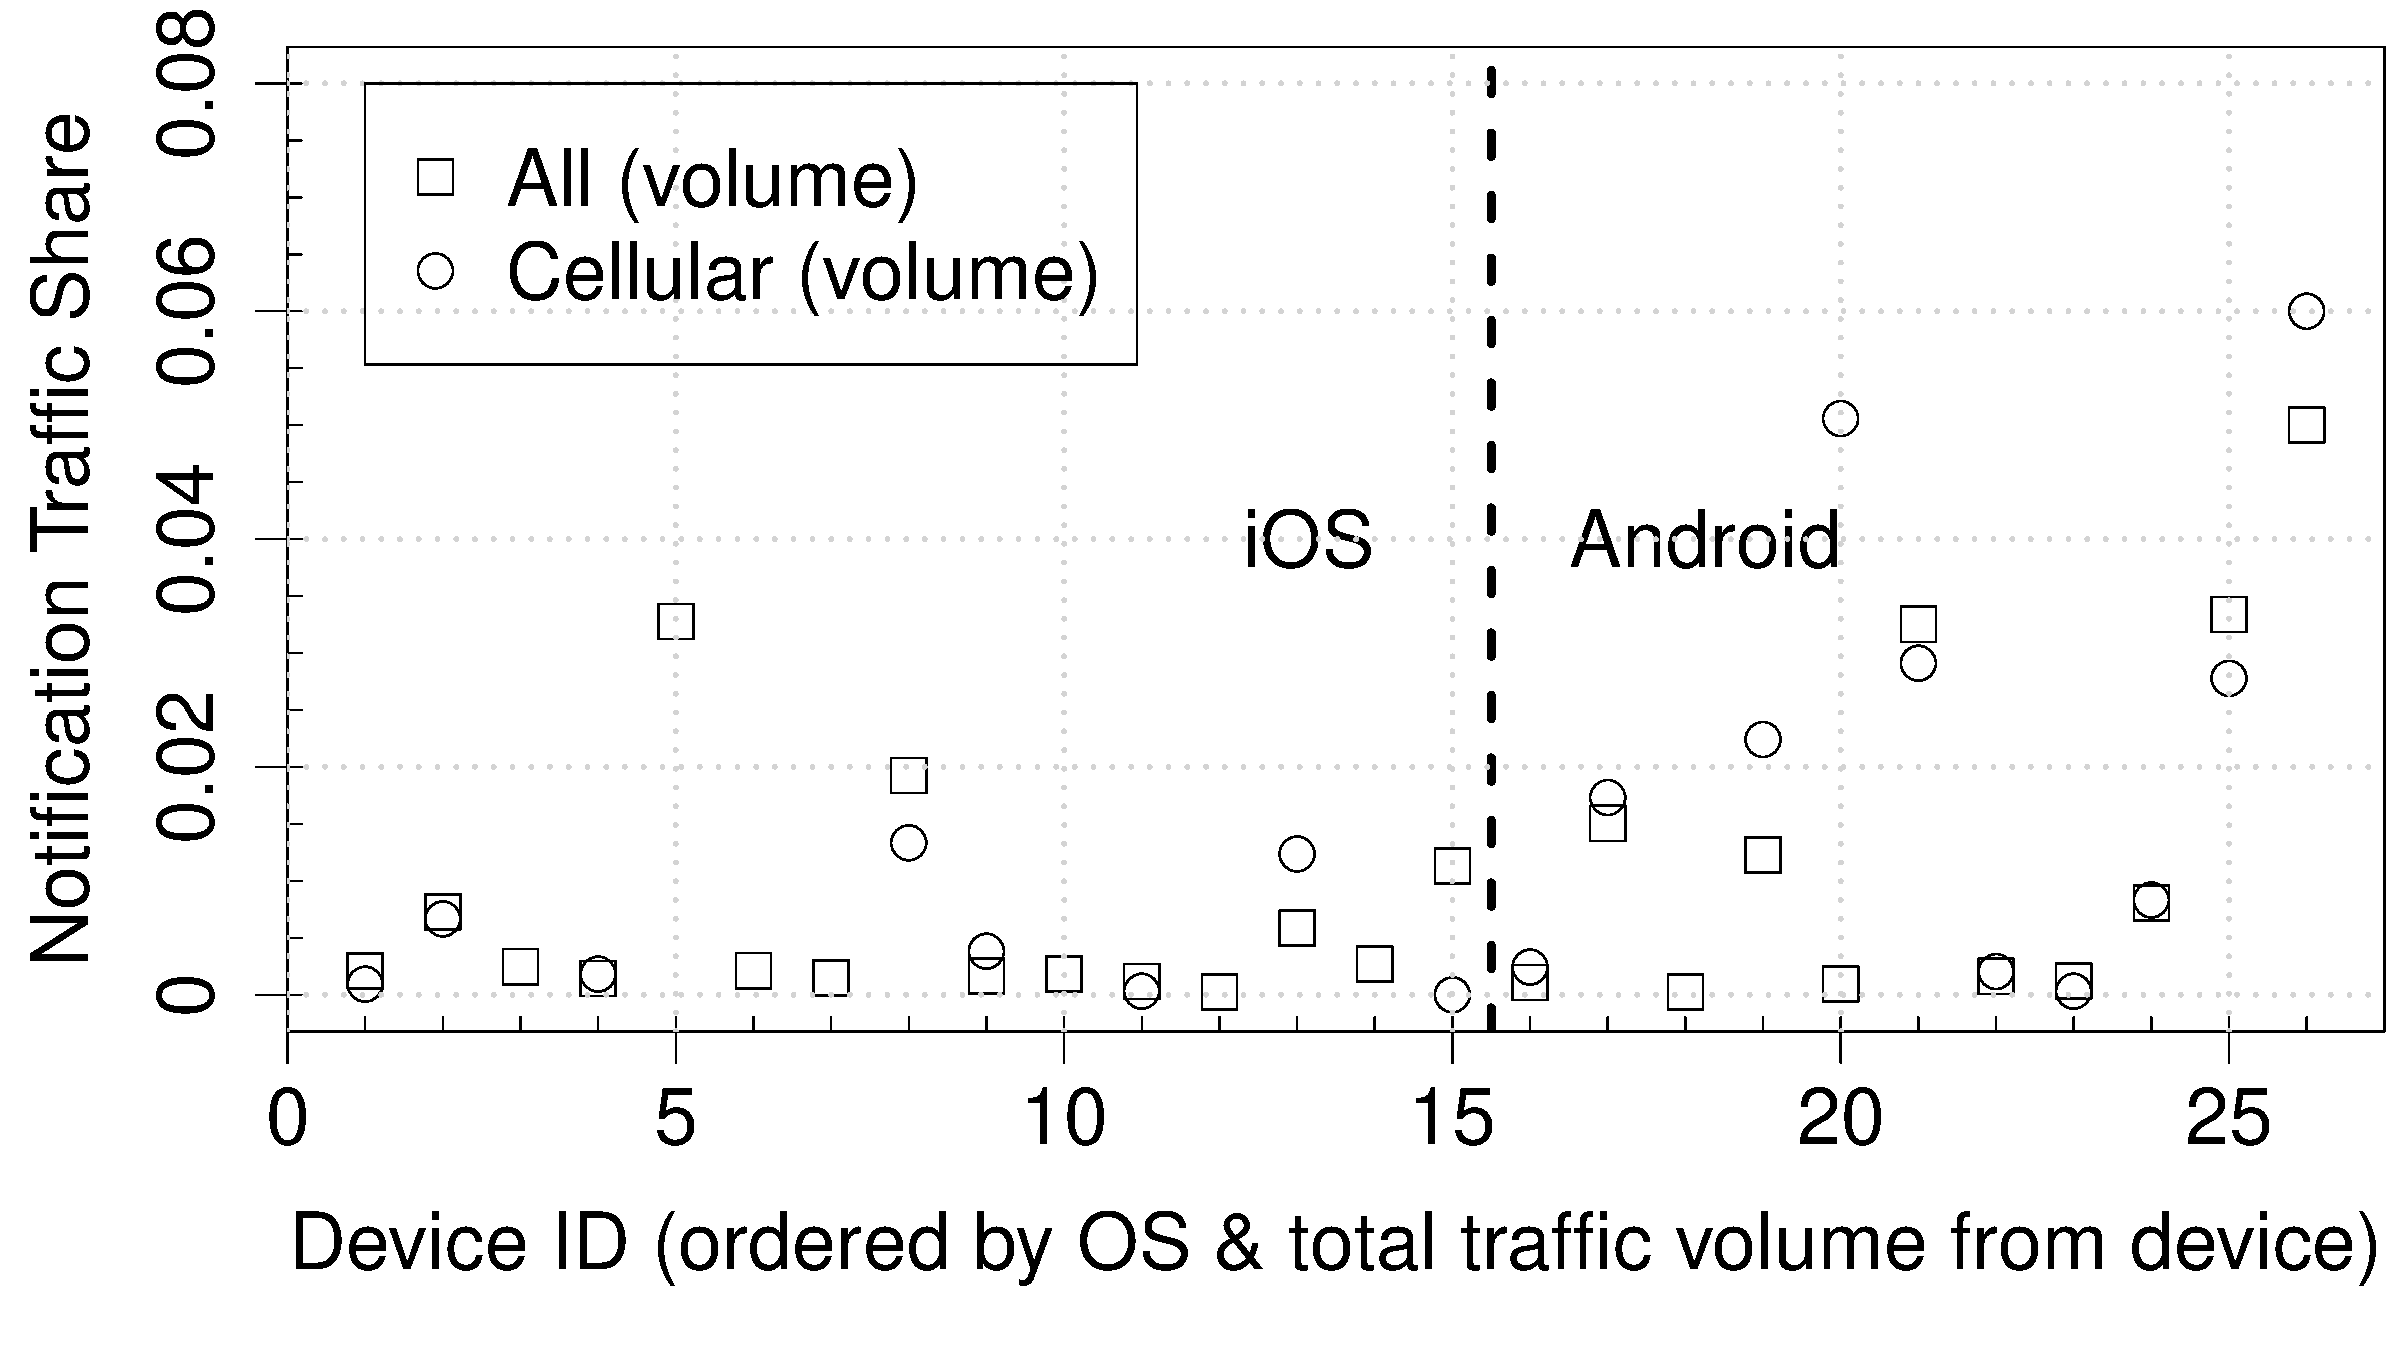
\includegraphics[width=\columnwidth]{plots/push_compare_trafficshare.pdf}
\caption{Traffic share of push notifications. \emph{Push notifications are responsible for less than 5\% of the traffic volume on most devices.}}
\label{fig:push-traffic-share}
\end{figure}

To analyze the volume of notification messages, we plot the share of notification messages as a fraction of total traffic from the device in \fref{fig:push-traffic-share}.
We observe that the notification messages are responsible for less than 4\% of the traffic volume on most Android and iOS devices. 
In \fref{fig:push-traffic-share}, we also plot the share of notification messages when the device exchanged data over cellular networks. 
We observe that there is no significant difference in the traffic share of notification messages when the device used cellular traffic. 
\tbd{Why do we care?}

To further analyze the source of the notification messages we analyzed the DNS lookups that were performed before the connections for receiving notification messages was established. 
We observed that the servers that pushed content to iOS devices correspond to the DNS requests that match the pattern \emph{*courier.push.apple.com} and \\ \emph{*courier-push-apple.com.akadns.net}.
For the android devices we observe that the DNS requests match the pattern\\ \emph{*talk.google.com}. 

In summary, we detail the behavior of the notification services using controlled experiments and the \mobWild dataset.  
We observe that push notifications consume a small fraction of the data and exhibit a heavy tail for the time between successive messages. 
We also observe that the frequency of notification messages was agnostic of the time of the day. 
Furthermore, notification messages were received by iOS devices even during the time interval the users had configured \emph{Do Not Disturb.}


% \begin{packedenumerate}
% \item How frequently do Push notifications take place in the wild?
% \item What is the impact of access technology on push notifications?
% \item What is the impact of the time of the day?
% \item What is the volume of push notification traffic?
% \item From which hosts are these notifications received?
% \end{packedenumerate}

%\subsection{Discussion}




% OLD TABLE WITHOUT IPHONE
% \begin{table}
% \begin{small}
% \begin{tabular}{|c|c|c|c|c|}
% \hline
% \multirow{2}{*}{\bf Application} & \multicolumn{4}{c|}{\bf Traffic Share in the first 24 hours}\tabularnewline
% \cline{2-5}
%      & iPad & iPod & Galaxy SIII & Nexus \tabularnewline
%      & (19 KB) & (21 KB) & (47 KB)& (97 KB)  \tabularnewline
% \hline
% Notifications & 0.54 & 0.53 & 0.35 & 0.88 \tabularnewline
% \hline
% Location & 0 & 0 & 0.26 & 0 \tabularnewline
% \hline
% SSL & 0 & 0 & 0.30 & 0.11 \tabularnewline
% \hline
% Mail & 0.05 & 0.07 & 0 & 0 \tabularnewline
% \hline
% HTTP & 0.13 & 0 & 0.09  & 0 \tabularnewline
% \hline
% UDP & 0.28 & 0.40 & 0.01 & 0.01 \tabularnewline
% \hline
% {\em total}& {\em 1.0} & {\em 1.0} & {\em 1.0} & {\em 1.0}\tabularnewline
% \hline
% \end{tabular}
% \end{small}
% \caption{Network usage in the first 24 hours after factory reset. \emph{Notifications contribute to the largest fraction of traffic volume across all devices.}}
% \label{tab:traffic-share-factory-reset}
% \end{table}

%While computing this distribution, we account the diversity in device usage in the following manner.
%For each device and each access technology we compute the 100 quantiles from 0.01 to 1.0 in steps of 0.01 of the time between successive push notifications. 
%We then use the median value of each quantile (from 0.01 to 1.0 in steps of 0.01) for a given access technology and operating system of the device.

% In \fref{fig:wild-inter-arrival-push} we present the time between successive push notifications for the 25 devices in our dataset. 
% As observed in \fref{fig:wild-cdf-push} we observe that the iOS devices receive push messages more frequently that the Android devices. 
% We also observe that the time between push notifications is higher for Android devices.
% The iOS devices prefer a cellular data connection for Push notification over \wifi \tbd{http://support.apple.com/kb/TS4264}. 
% However, in \fref{fig:wild-cdf-push} and \fref{fig:wild-cdf-push} despite this preference, we observe that the time between successive push notifications for iOS devices is higher over cellular networks in comparison to \wifi networks.  
% We observe that \tbd{SSL traffic} to mail servers was followed \tbd{x\%} after push notifications.
% This implies that higher usage of the device over \wifi may result in a higher number of notificatons received. 
% In \fref{fig:wild-inter-arrival-push}, device ID 
%Only if the cellular connection is not available or viable will the device switch to Wi-Fi for APNs connections.


\section{Application Characterization}
\label{sec:characterize-app}

  We now turn to measurements of specific popular iOS and Android applications. 
  When users install apps, they grant them Internet access without detailed knowledge of how that access will be used, including {\it how much} data is sent or accessed, {\it what} data is sent,  or {\it with whom} the app communications.
  ``How much'' is important to conserve both bandwidth caps and battery capacity: an app which consumes or produces too much data will waste bandwidth resources, while an app which consumes or produces data too frequently will prevent the device radio from going idle to save power.
  ``With whom'' is important to protect users from excessive tracking -- the more organization's servers an app connects to, the more organizations which are able to track user behavior, location, or other private data.
  Finally, ``what data'' is important because apps may unnecessarily leak personally identifiable information (PII) such as user email address, IMEI, contact information, or other stored data either to the app provider or worse, to any eavesdropper on a public WiFi connection.
  We  report on our findings in all three of these dimensions for the iPhone and Android apps in our study.

\subsection{Bandwidth and Radio Usage}

  {\bf In the Wild.}
    \begin{itemize}
      \item Stats on how much bandwidth each user used; time of day; how frequent...
    \end{itemize}

  {\bf Android Apps.}
    To dig in to the root cause of these usage patterns, we also did an `app-by-app` analysis of network usage to see if most bandwidth consumption/radio time was the result of a few heavy applications, with most applications relatively idle, or whether usage was divided amongst all applications equally.
    In Figure~\ref{fig:app-by-app-usage}, we plot the CDF of total bytes transferred by each app in our study, one line for the top-100 Google Play apps we tested manually, and another for the top 2000 apps, tested automatically, from a third-party market.
    We see that...\tbd{Amy...}
    Regarding radio usage,...\tbd{Do we even have time to do this? I don't remember the exact metrics we used for the MobiSys submission.}

  {\bf iPhone Apps.}

\subsection{Third Party Servers}
  Many free applications support themselves financially by serving ads or providing resources for third parties to track user behavior.
  We now explore how many servers are contacted by a given app (\ie{} how many providers are tracking a user with this app) -- most of these typically for ads, tracking, or analytics -- as well as how much data is transferred to and from these servers (\ie{} how much does this traffic impact the user's data cap?).

  {\bf In the Wild.}
  We first consider the overall impact of these ads, analytic, and tracking services on typical user behavior in our IRB study...
  \tbd{Ashwin...}

\begin{figure}[t]
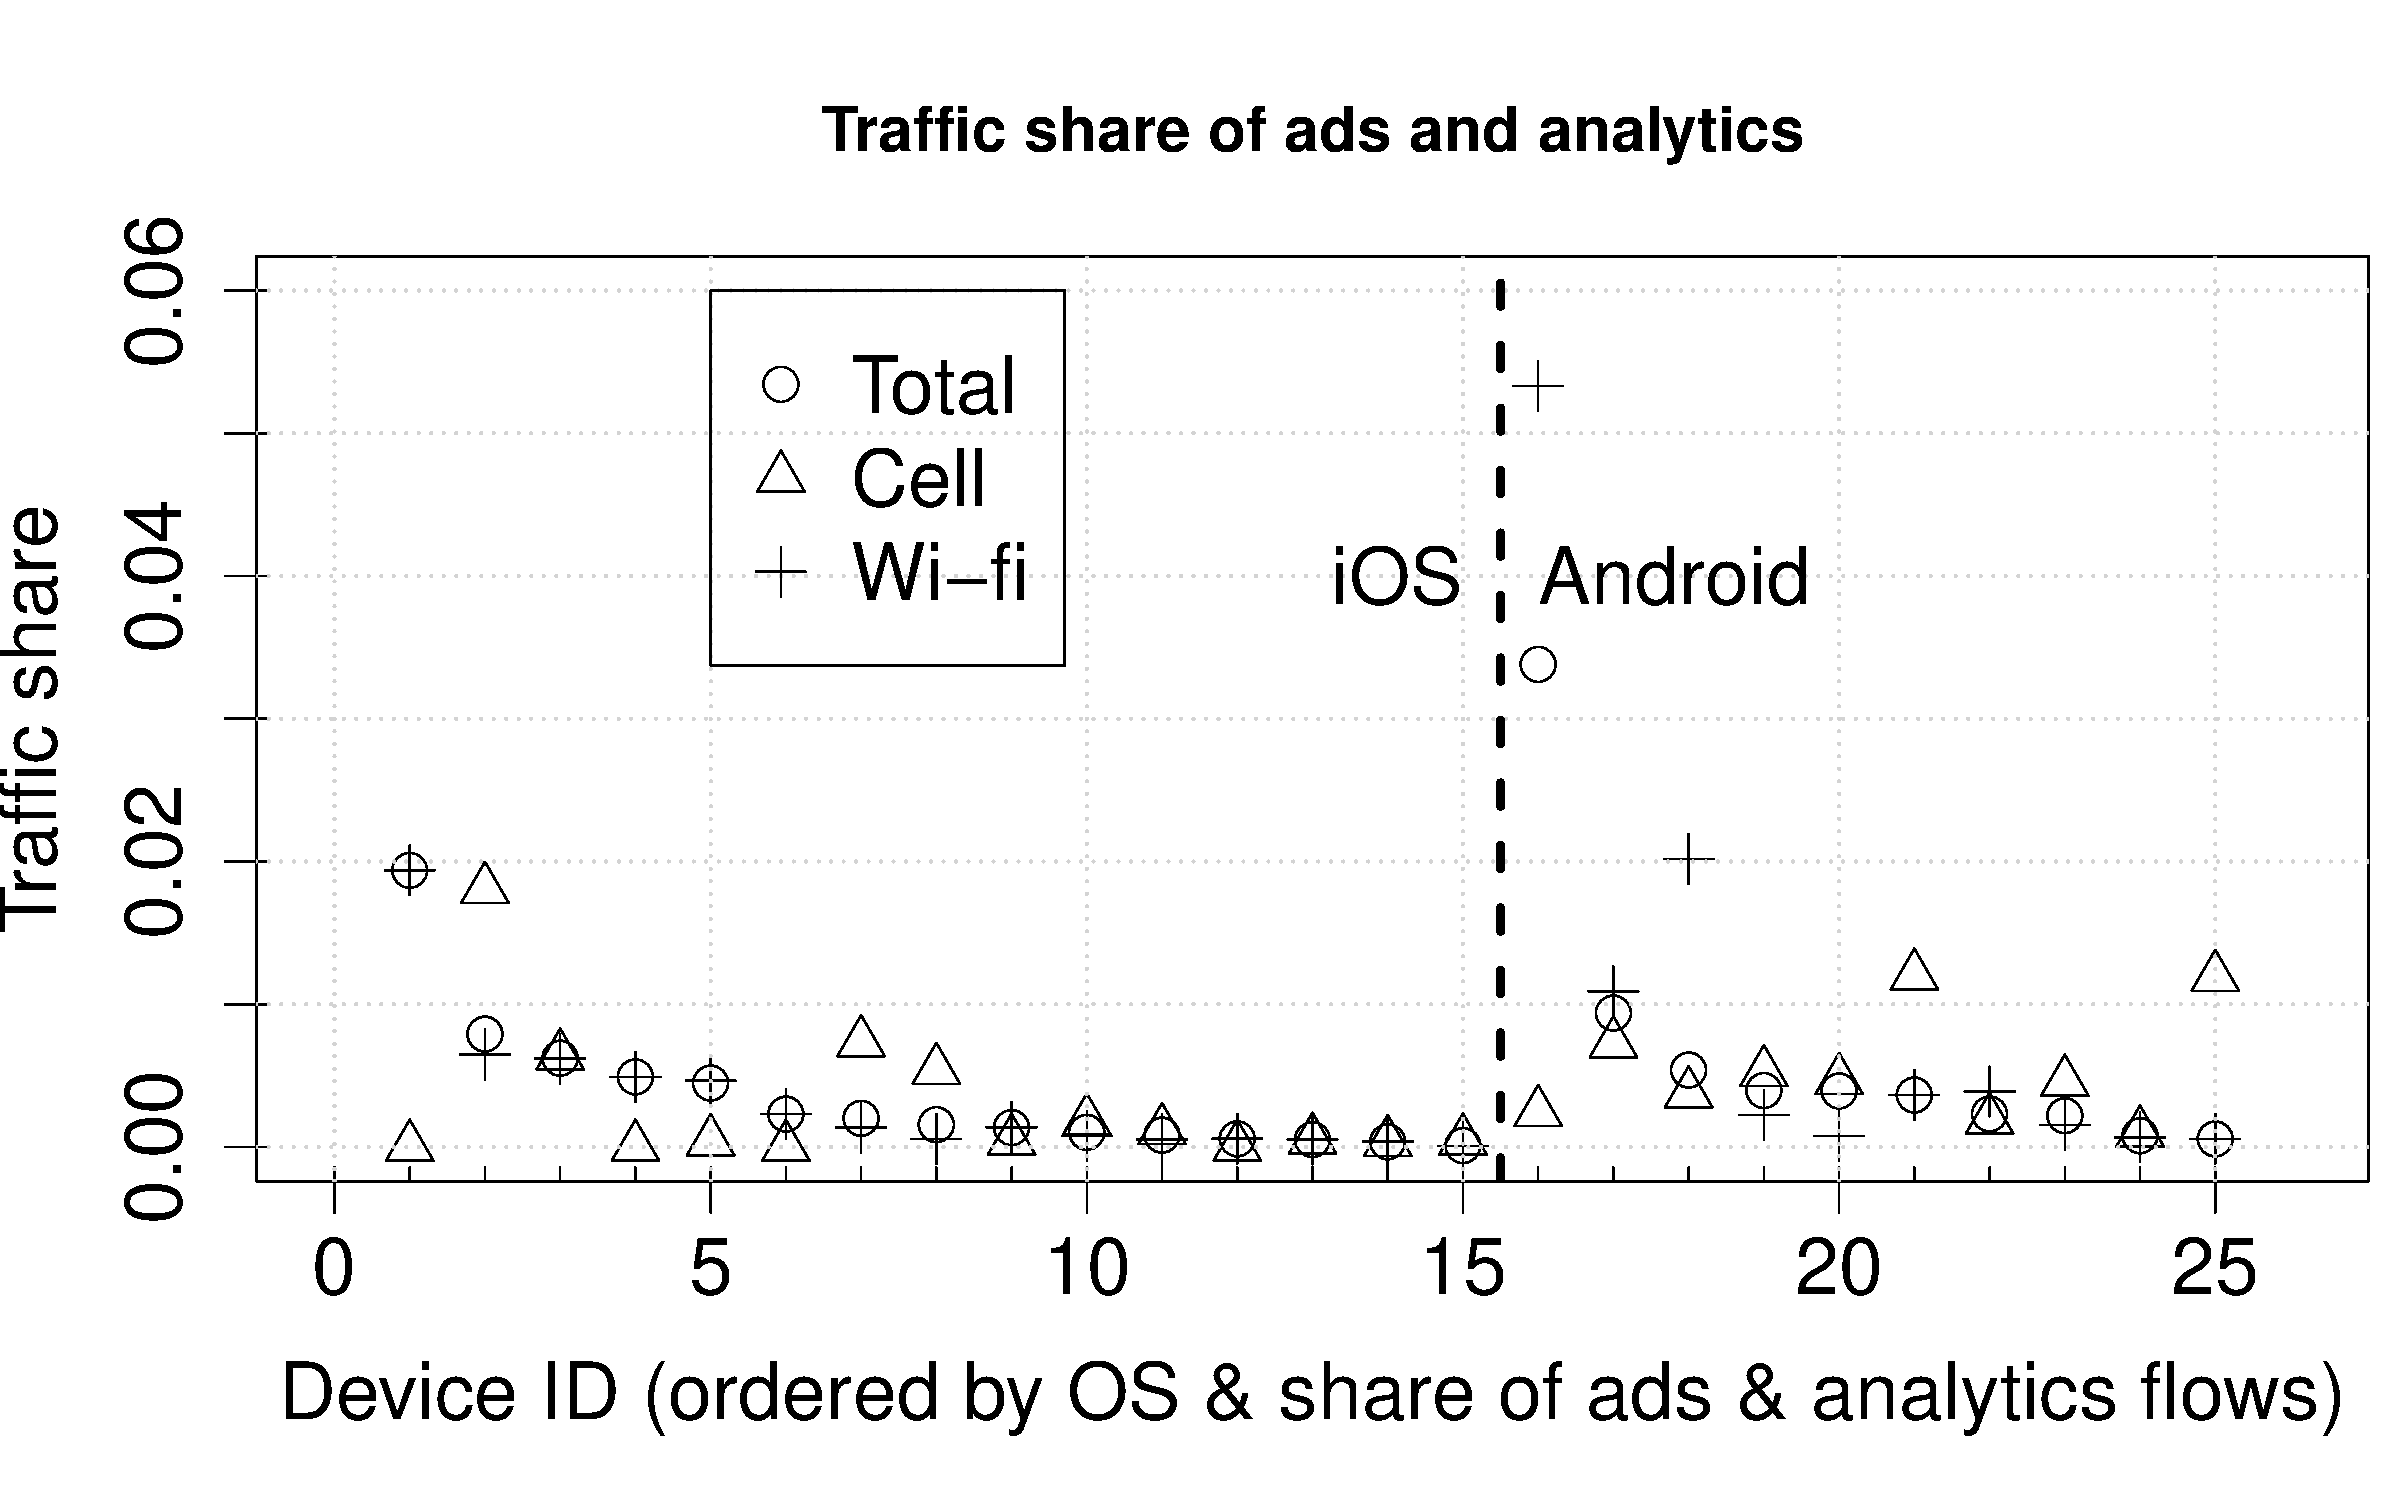
\includegraphics[width=\columnwidth]{plots/ad_share_bytes.pdf}
\caption{Fraction of traffic volume because of Ads and Analytics. \emph{\tbd{Check for id1 and id25}}}
\label{fig:description}
\end{figure}

\begin{figure}[t]
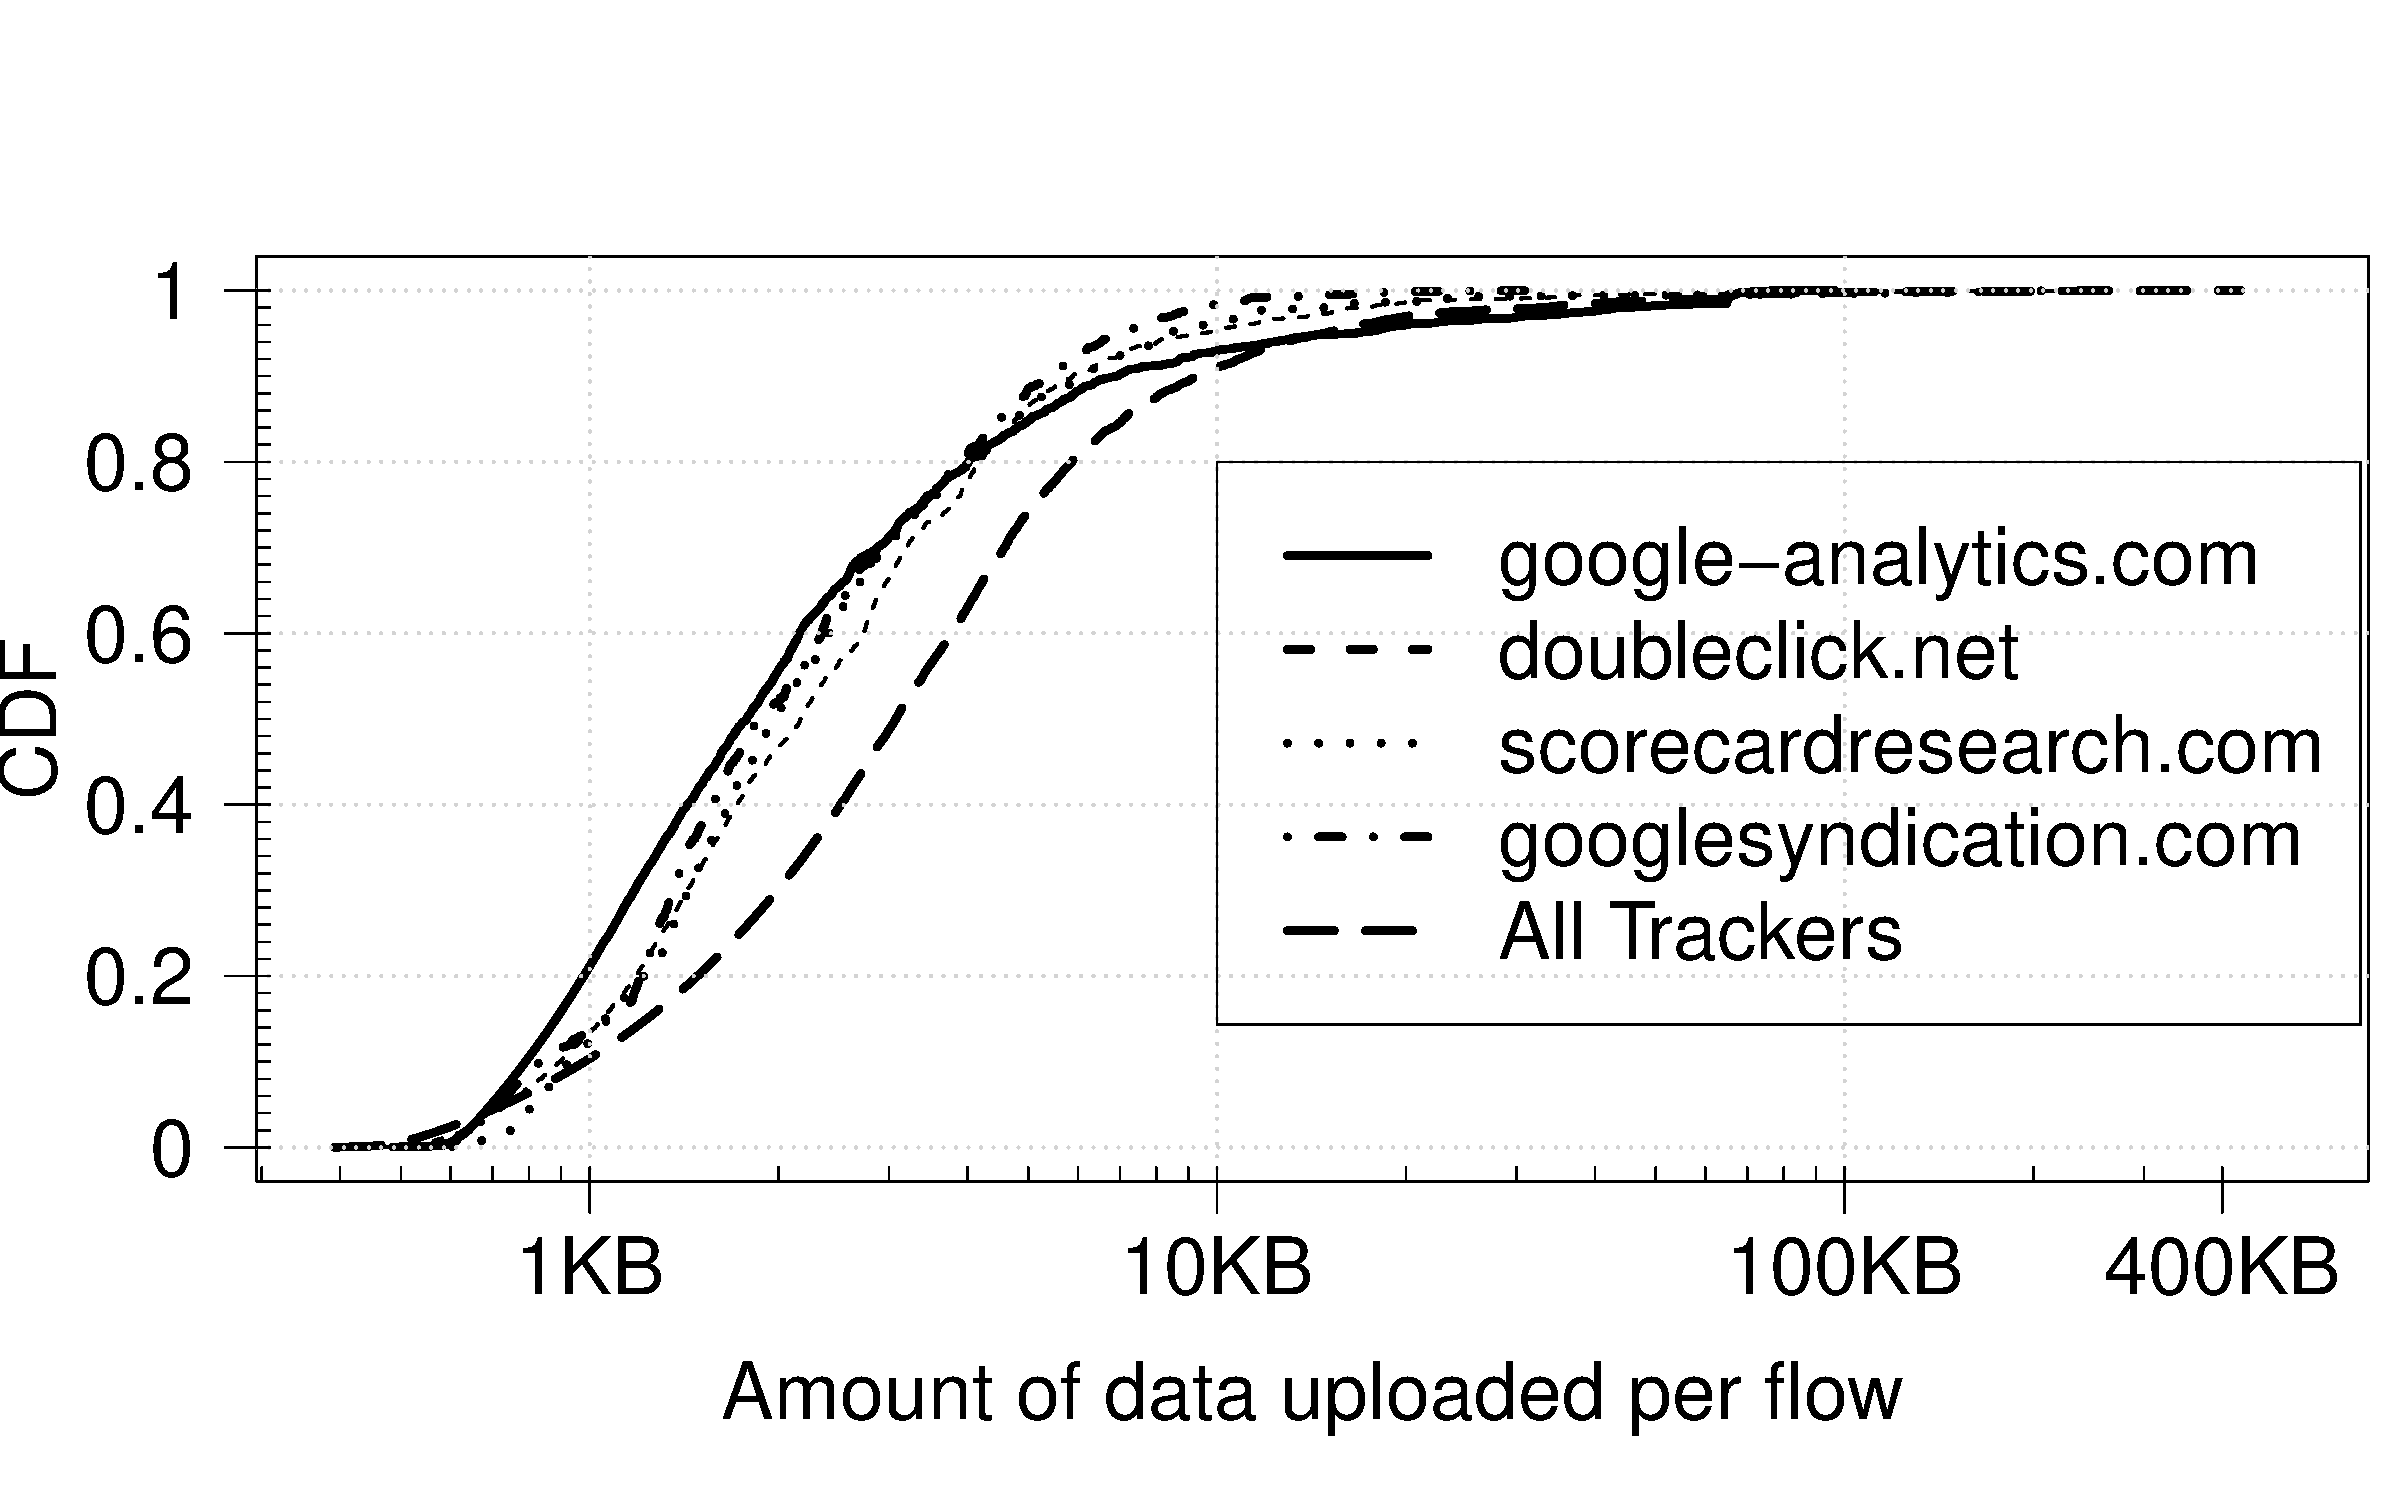
\includegraphics[width=\columnwidth]{plots/distrib_ad_uploads.pdf}
\caption{Distribution of bytes uploaded by ads and analytics sites. \emph{The distribution of bytes uploaded by all ads and analytics sites and the top four ads sites based on traffic volume across all users}.}
\label{fig:description}
\end{figure}

\begin{figure}[t]
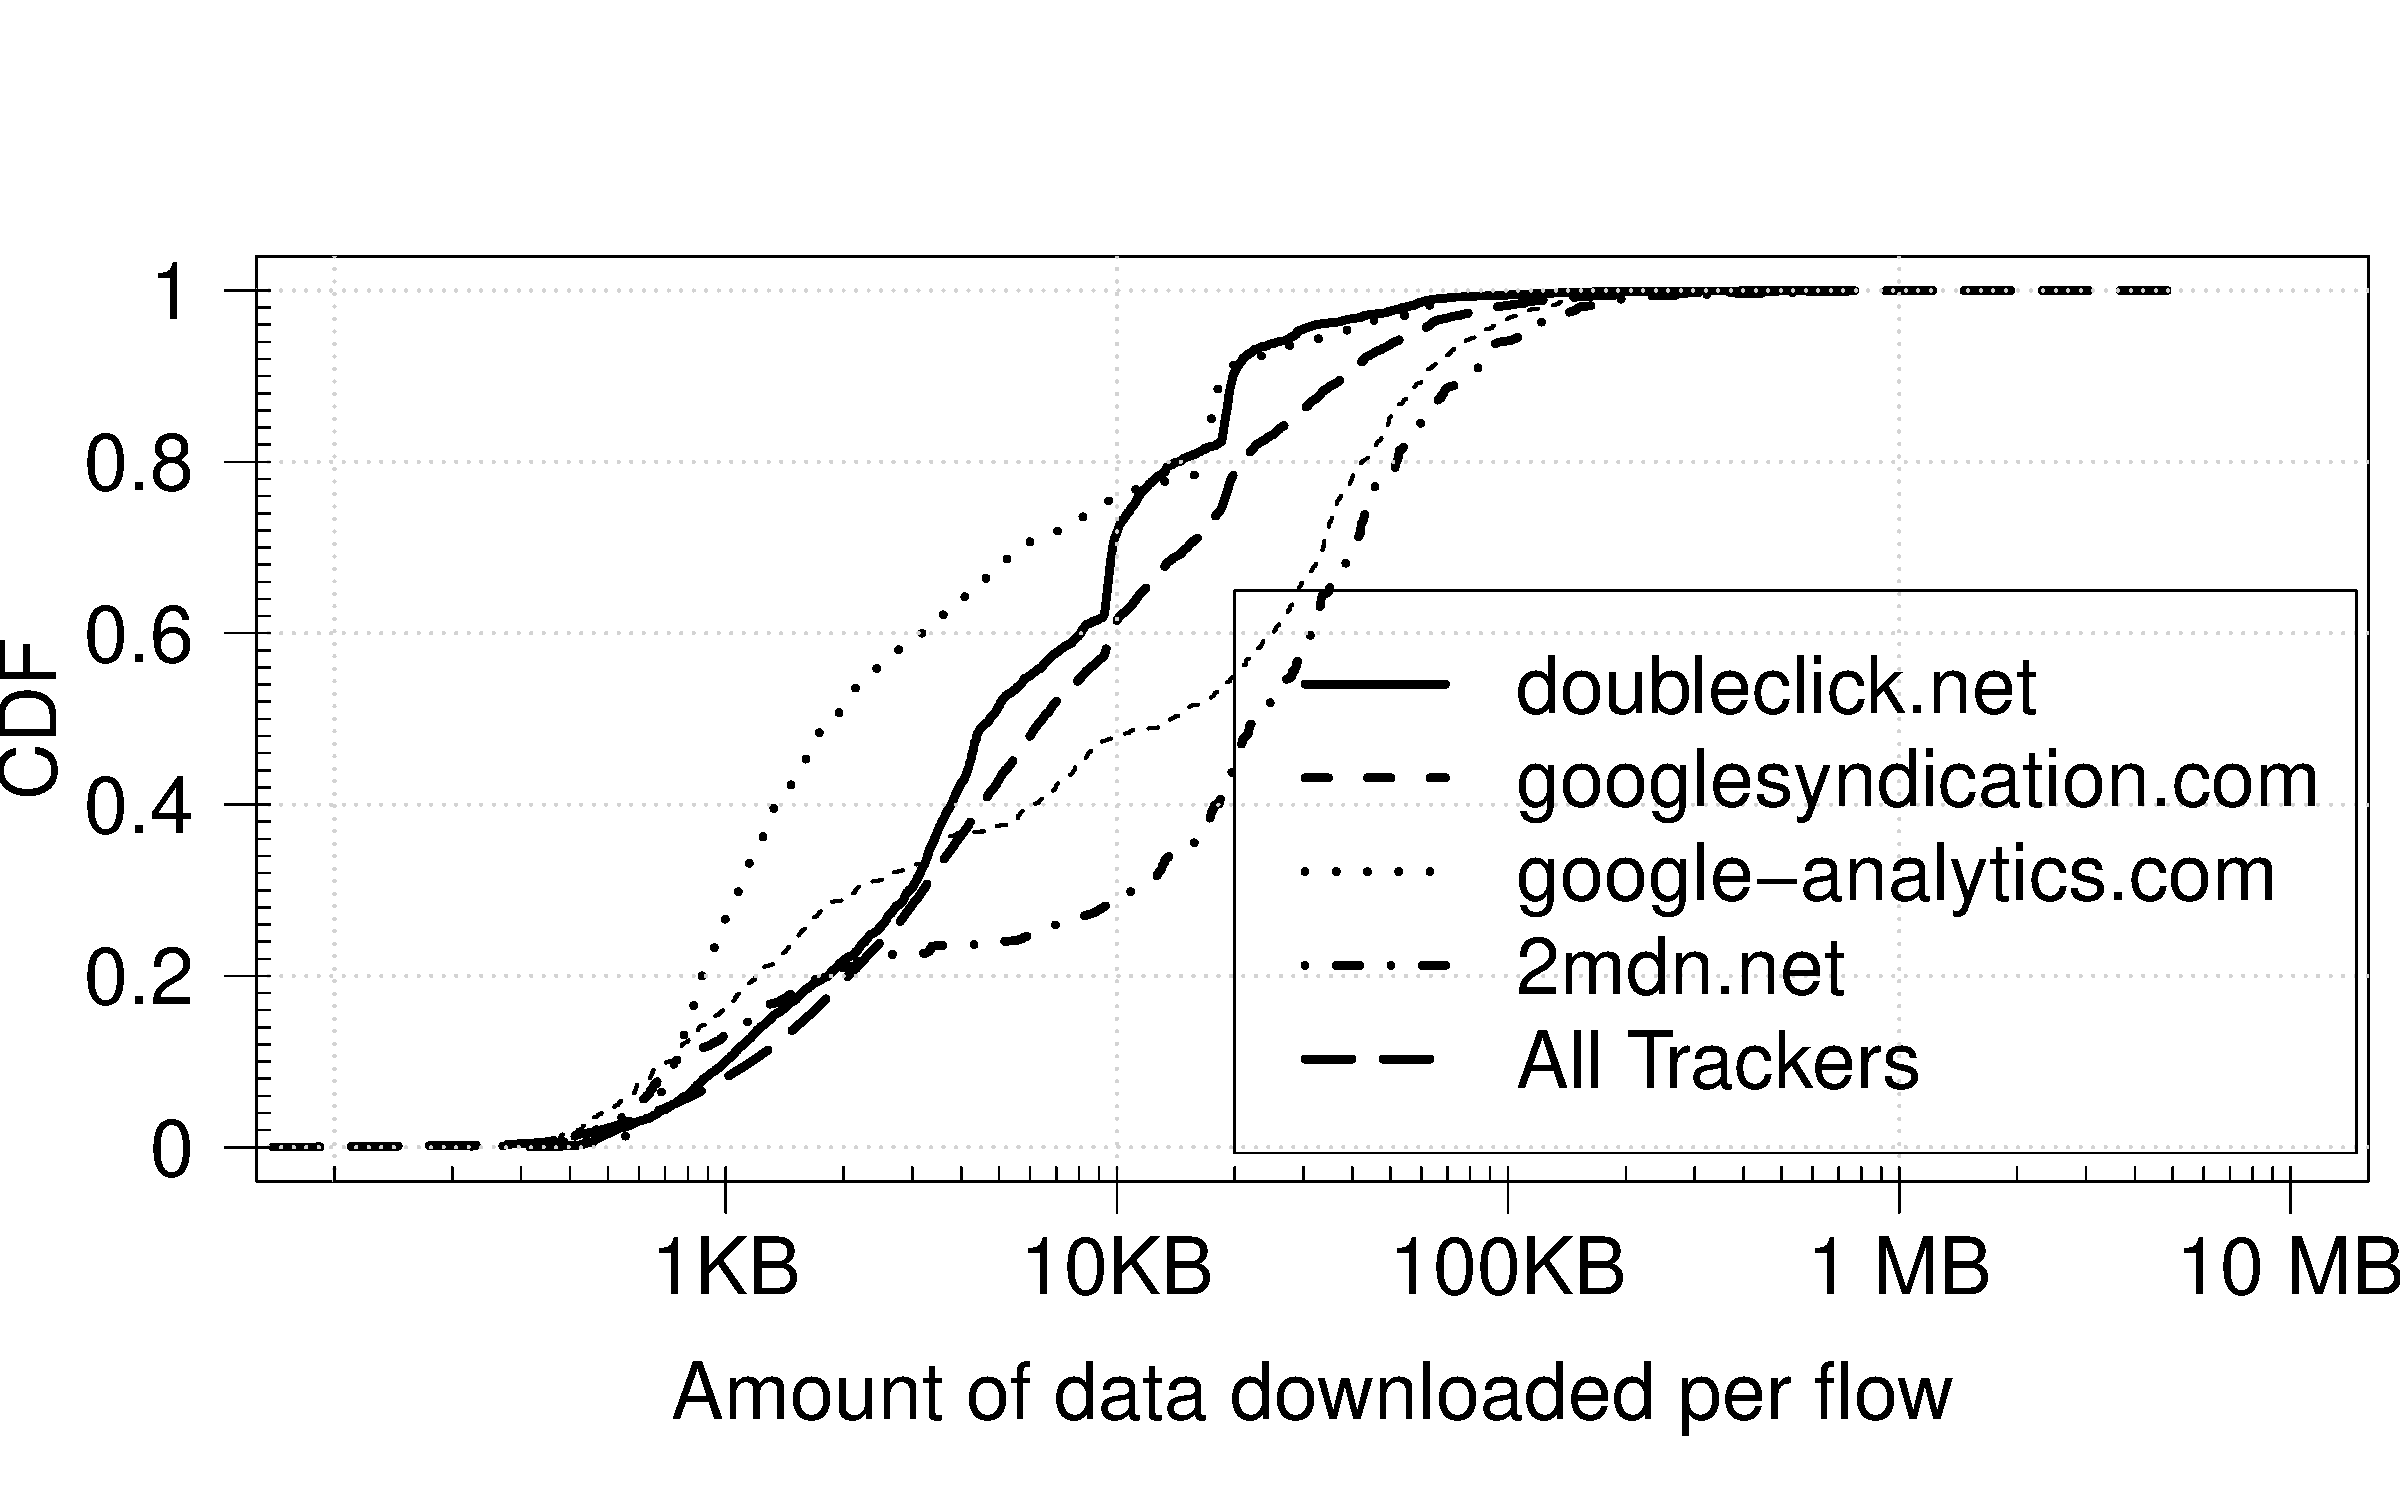
\includegraphics[width=\columnwidth]{plots/distrib_ad_downloads.pdf}
\caption{Distribution of bytes downloaded by ads and analytics sites. \emph{The distribution of bytes uploaded by all ads and analytics sites and the top four ads sites based on traffic volume across all users}.}
\label{fig:description}
\end{figure}

\begin{table}[t]
\centering
\begin{small}
\begin{tabular}{|p{0.35\columnwidth}|p{0.1\columnwidth}|p{0.15\columnwidth}|p{0.1\columnwidth}|}
\hline
\multirow{2}{*}{\bf Tracker} & \multicolumn{3}{c|}{\bf Number of devices tracked}\tabularnewline
\cline{2-4}
   &  {\bf Total} & {\bf Android} & {\bf iOS} \tabularnewline
\hline
doubleclick.net & 25 & 11 & 14 \tabularnewline
\hline
google-analytics.com   & 25 & 11 & 14 \tabularnewline
\hline
googlesyndication.com  & 22 & 10 & 12 \tabularnewline
\hline
admob.com  & 21 & 10 & 11 \tabularnewline
\hline
scorecardresearch.com &  21 & 10 & 11 \tabularnewline
\hline
2mdn.net  &  20 & 9 &  11 \tabularnewline
\hline
atdmt.com  & 18 & 9 &  9 \tabularnewline
\hline
imrworldwide.com & 18 &  9 &  9 \tabularnewline
\hline
flurry.com & 17 & 7 &  10 \tabularnewline
\hline
googleadservices.com  & 17 & 8 &  9 \tabularnewline
\hline
\end{tabular}
\end{small}
\caption{The top 10 ads and analytics sites that tracked the devices in our dataset.
\emph{Two trackers, \emph{doubleclick.net} and\emph{google-analytics.com}, were tracking all the 25 devices in our dataset.}}
\label{tab:top_trackers}
\end{table}


\begin{table*}[t]
    \begin{tabular}{l|l|l|l|l|l|l|l|l|l|l}
       Dataset&Platform&Proto&\# Apps&Email&Location&Username&Password&Android ID&Contacts&IMEI\\
       \hline
       Google Play&Android&HTTP&100&?&10 (10\%)&7 (7\%)&1 (1\%)&21 (21\%)&0 (0\%)&13 (13\%)\\
       \hline
       Third Party&Android&HTTP&908&?&32 (3.5\%)&?&0 (0\%)&95 (10.4\%)&4 (0.4\%)&48 (5.3\%)\\
       \hline
       App Store&iPhone&HTTP&100&?&?&?&?&?&?&?\\
    \end{tabular}
    \caption{\label{tbl:pii}Summary of personally identifiable information leaked in plaintext (HTTP) by Android and iPhone apps.}
  \end{table*}
  

  {\bf Android Apps.}
  When we inspect the data from our controlled study, we see that some apps contact a large number of external servers while others contact significantly fewer.
  In Figure~\ref{fig:android-cdns}, we show both the total number of servers contacted (solid lines) as well as the number of organizations contacted (dotted lines) for both the top-100 Google Play dataset and the top-2000 third-party dataset.
  To quantify ``organizations contacted'', we performed whois lookups on all servers contacted and mapped them to an organization name, allowing us to tighten our upper bound on the number of companies/entities able to track the user through a single app.
  Returning to the figure, we see...~\ref{fig:android-cdns}...\tbd{Amy...}


  {\bf iPhone Apps.}
  \tbd{Shen...}

\subsection{Personally Identifiable Information}
 
  Finally, we turn to information leaked by individual applications. We do not report on data leaked for our real users here, but only the data leaked by our controlled apps in isolation.
  We created fake user accounts on the test phones for a fake user named ``Tess Droid'', with fake contact information and fake Twitter and Facebook accounts. 
  We were then able to check that none of this data ever was released over the network, either in plaintext (HTTP) or encrypted (HTTPS, see \S\ref{sec:bumping}).
  
  We consider data to be `leaked' when any personally identifiable information -- email address, phone number, IMEI number -- is sent across the network under HTTP or HTTPS.
  Some of this information may be relevant to the app -- \eg{}, many apps legitimately require email access. 
  However, none of this information should ever travel across the network in plaintext (HTTP), which we see violated in serveral cases.

  In Table~\ref{tbl:pii}, we see the type of PII leaked for both Android and iPhone apps.
  For Android apps, IMEI and Android ID are the most commonly leaked forms of PII in both the Google Play and third-party dataset.
  Although not popularly thought of as ``private'' data, each of these identifiers are globally unique: IMEI is a unique identifier tied to a phone, and an Android ID is an identifier tied to a user's Google Account, used across many services on the Internet. 
  Consequently, either of these datapoints can be used to track or correlate a user's behavior across all sites the user visits that sell or collaborate with tracking data: a user's behavior on one site can easily be linked to their behavior on any other site they visit.
  With Android ID being tracked by between 10 and 20\% of apps in our study, and IMEI being tracked by between 5\% and 13\% of apps in our study, this suggests that global user tracking across collaborating services can be easily achieved today just by using this identifier.
  \tbd{...}

  Other informaiton like contacts, email, and passwords were rarely leaked in the clear, but all were leaked on occaision, suggesting that stricter monitoring of Android app behavior is needed -- contrastingly, no iPhone apps (which are manually given clearance by Apple before hitting the iPhone store) leaked passwords in plaintext~\tbd{is this true.}

  Moving to iPhone apps, \tbd{...}
%\subsection{Characterize Facebook Applications}

%Why Facebook was chosen?

%What do we observe ?

%What do we see in the User Agent Fields. 




\section{Behavior of Networks}

\subsubsection{Controlled Experiments}

\subsubsection{In the Wild}

We ignore connections from the same network and ISP in which our servers were placed.


\begin{figure}[t]
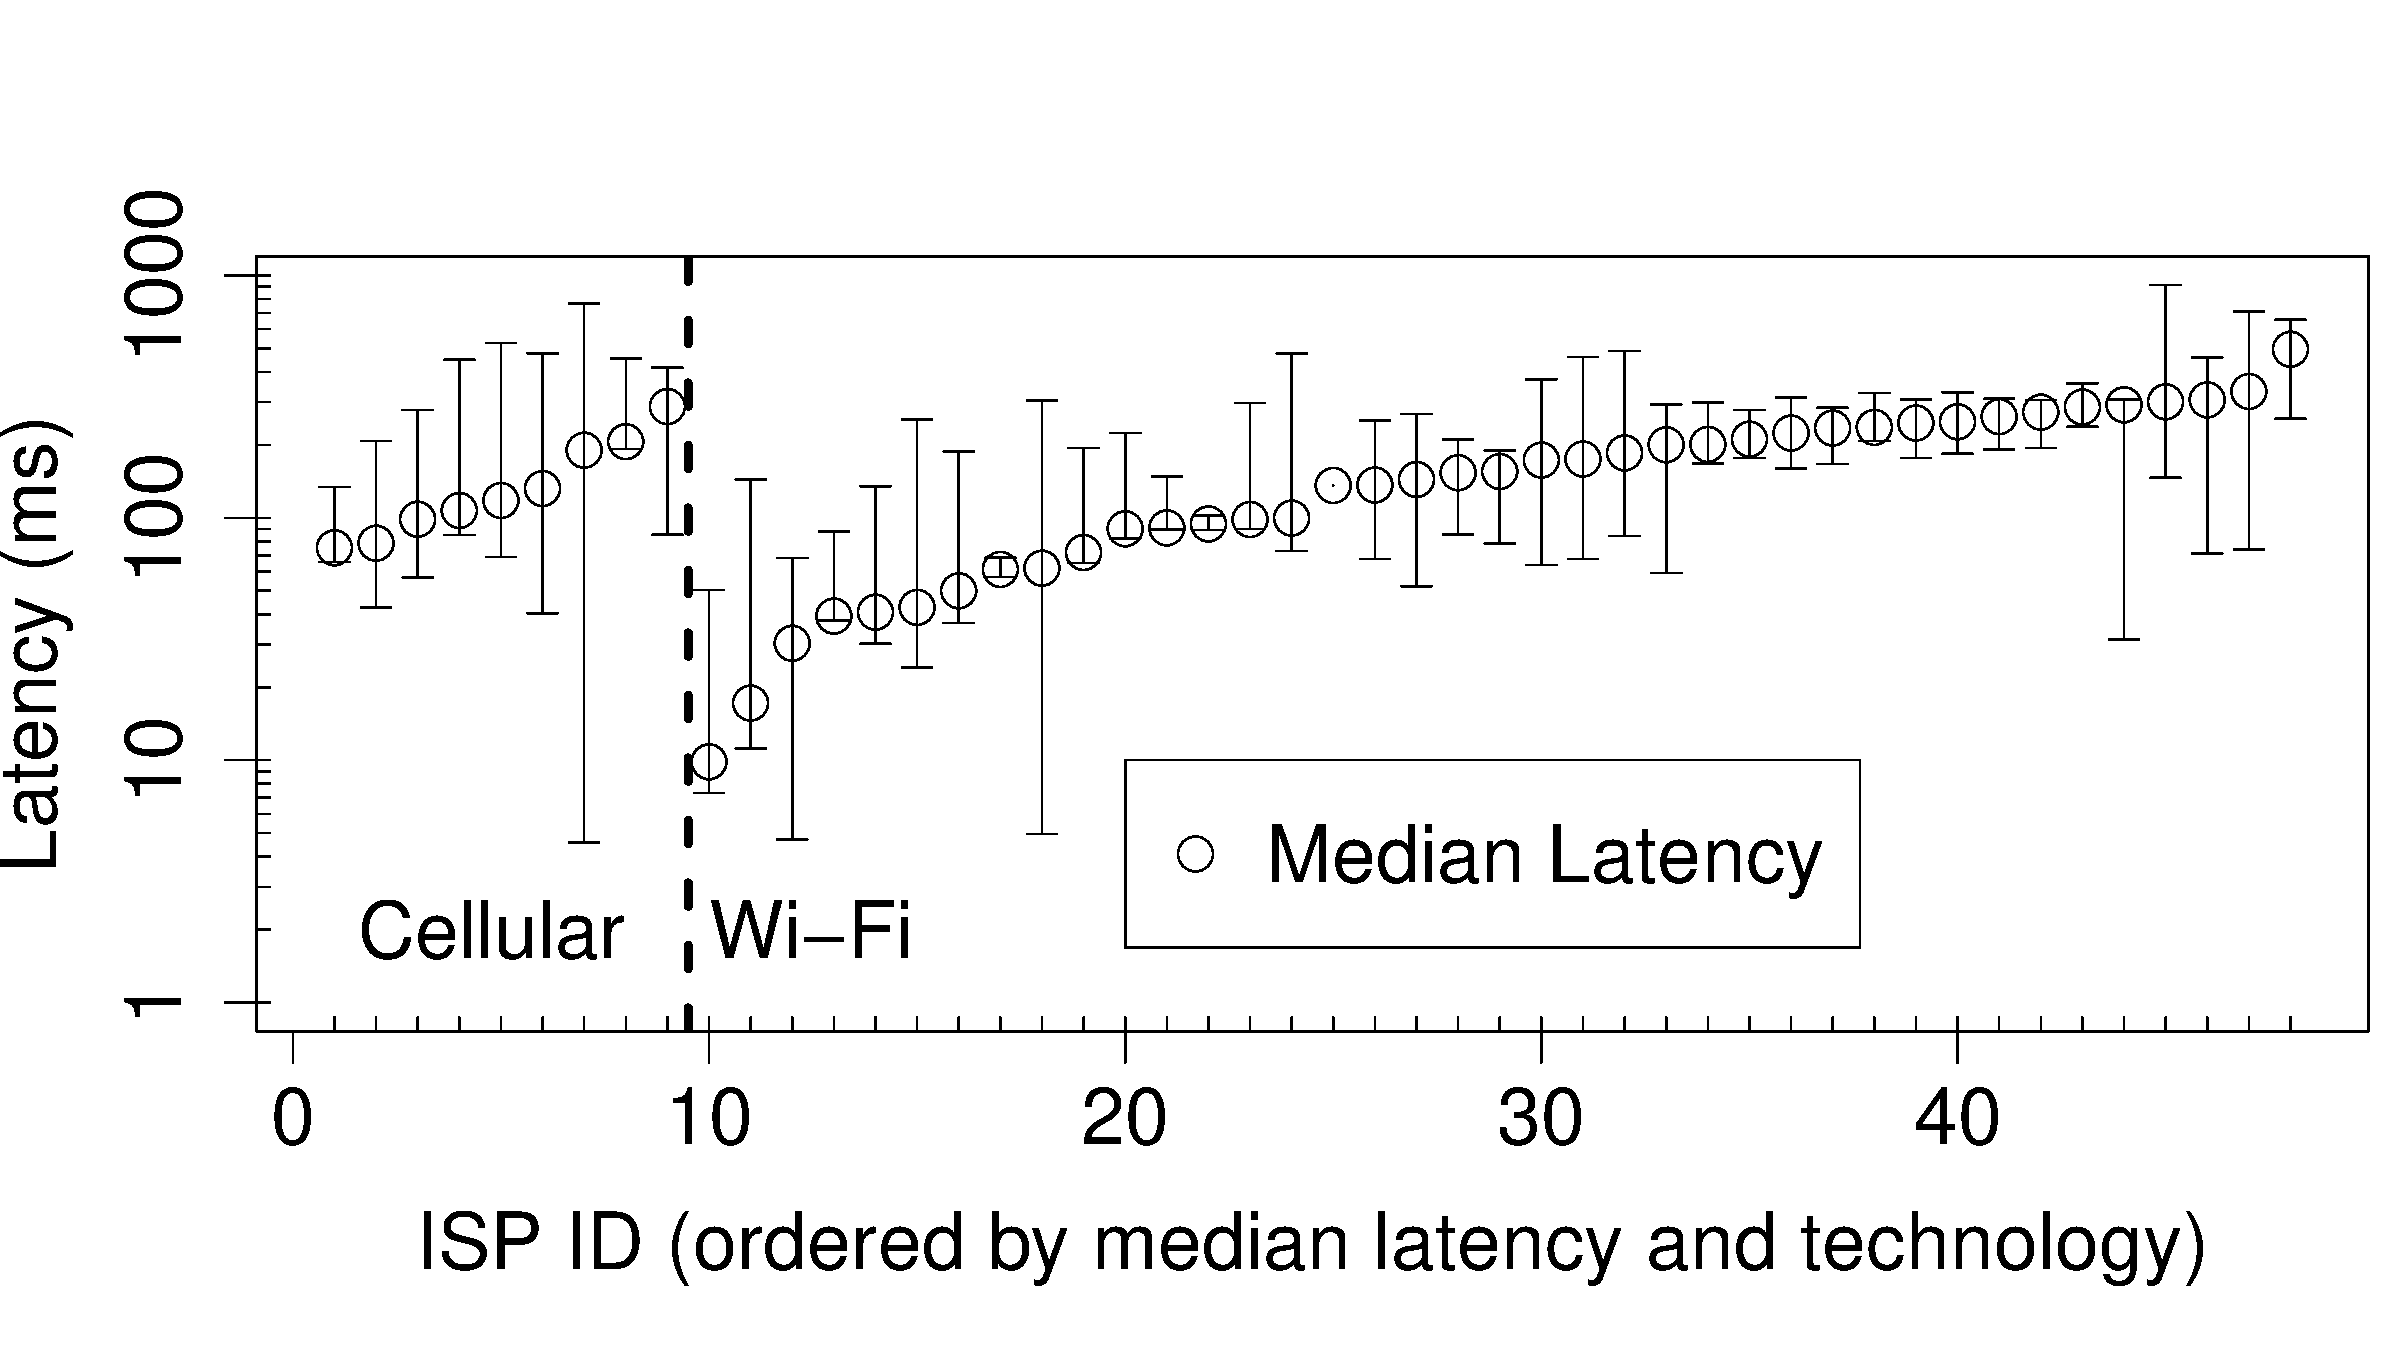
\includegraphics[width=\columnwidth]{plots/latency_isp_whisker.pdf}
\caption{One-way latency from VPN server to mobile devices. \emph{Connections from cellular ISPs suffer a higher delay compared to Wi-Fi ISPs. The delays from Cellular ISPs is comparable to connecting from a Wi-Fi ISP in another country. Error bars indicate the 91st and 9th percentile}.}
\label{fig:latency-across-isps}
\end{figure}


\begin{figure}[t]
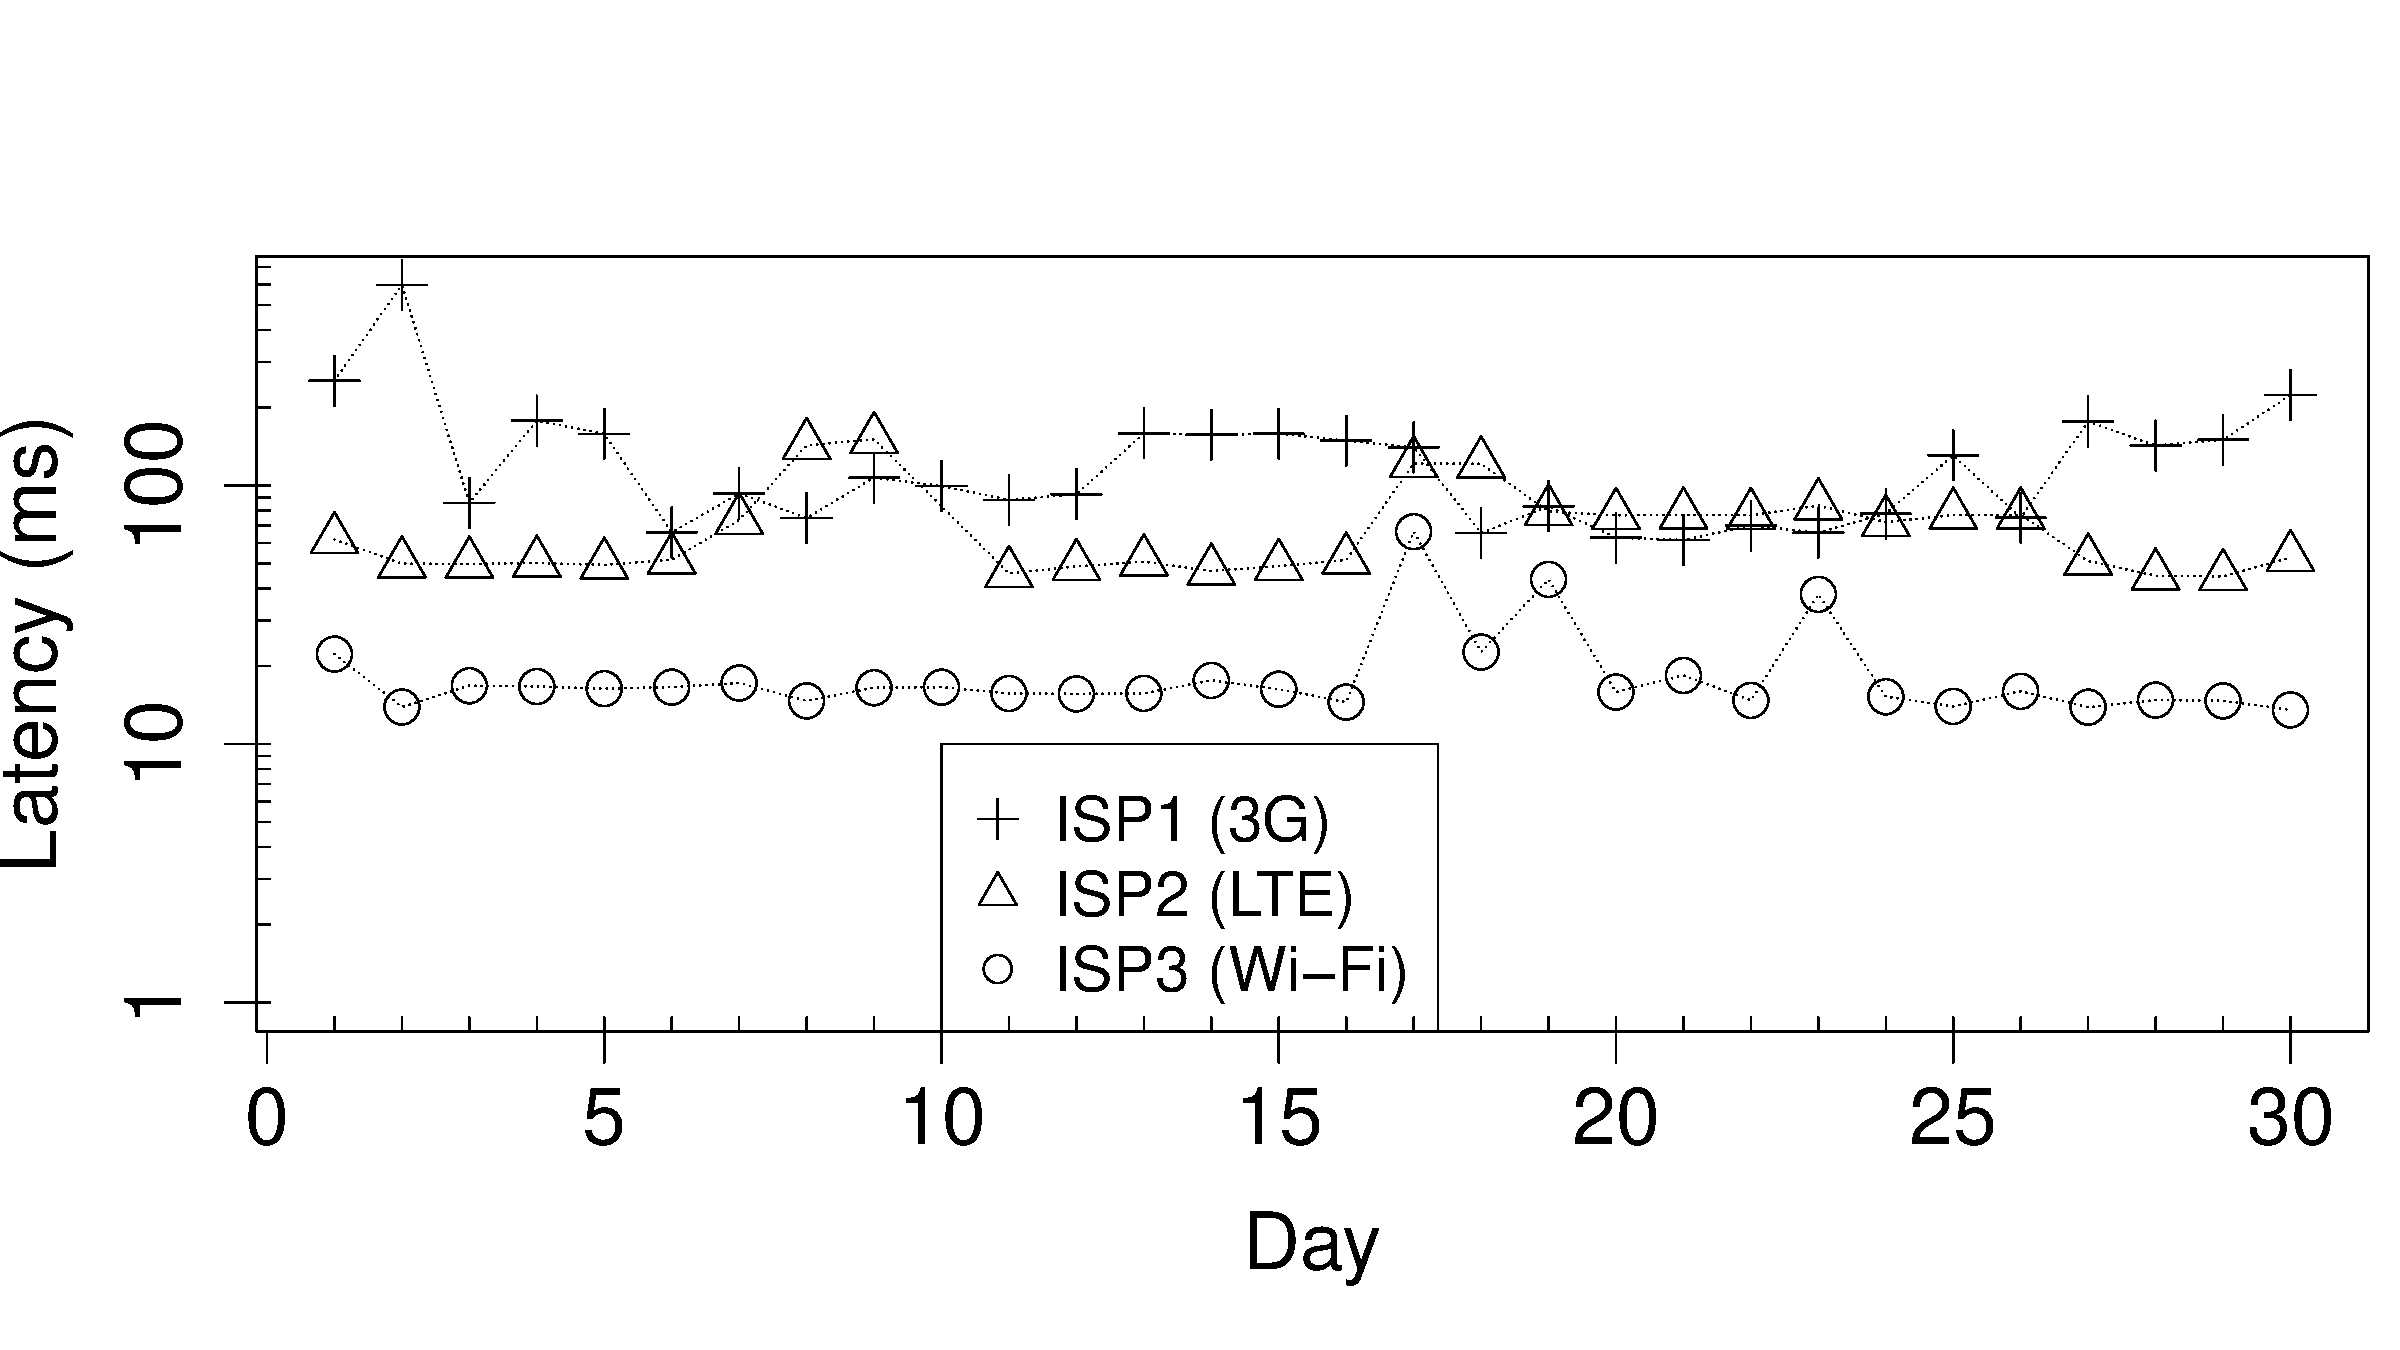
\includegraphics[width=\columnwidth]{plots/compare_isp_latency.pdf}
\caption{Comparison of ISPs that serve the same user during a 30 day time period. \emph{The LTE service provider has a smaller latency to the 3G provider. The smallest latency is observed by in the home Wi-Fi network.}}
\label{fig:compare-isp-latency}
\end{figure}

\begin{figure}[t]
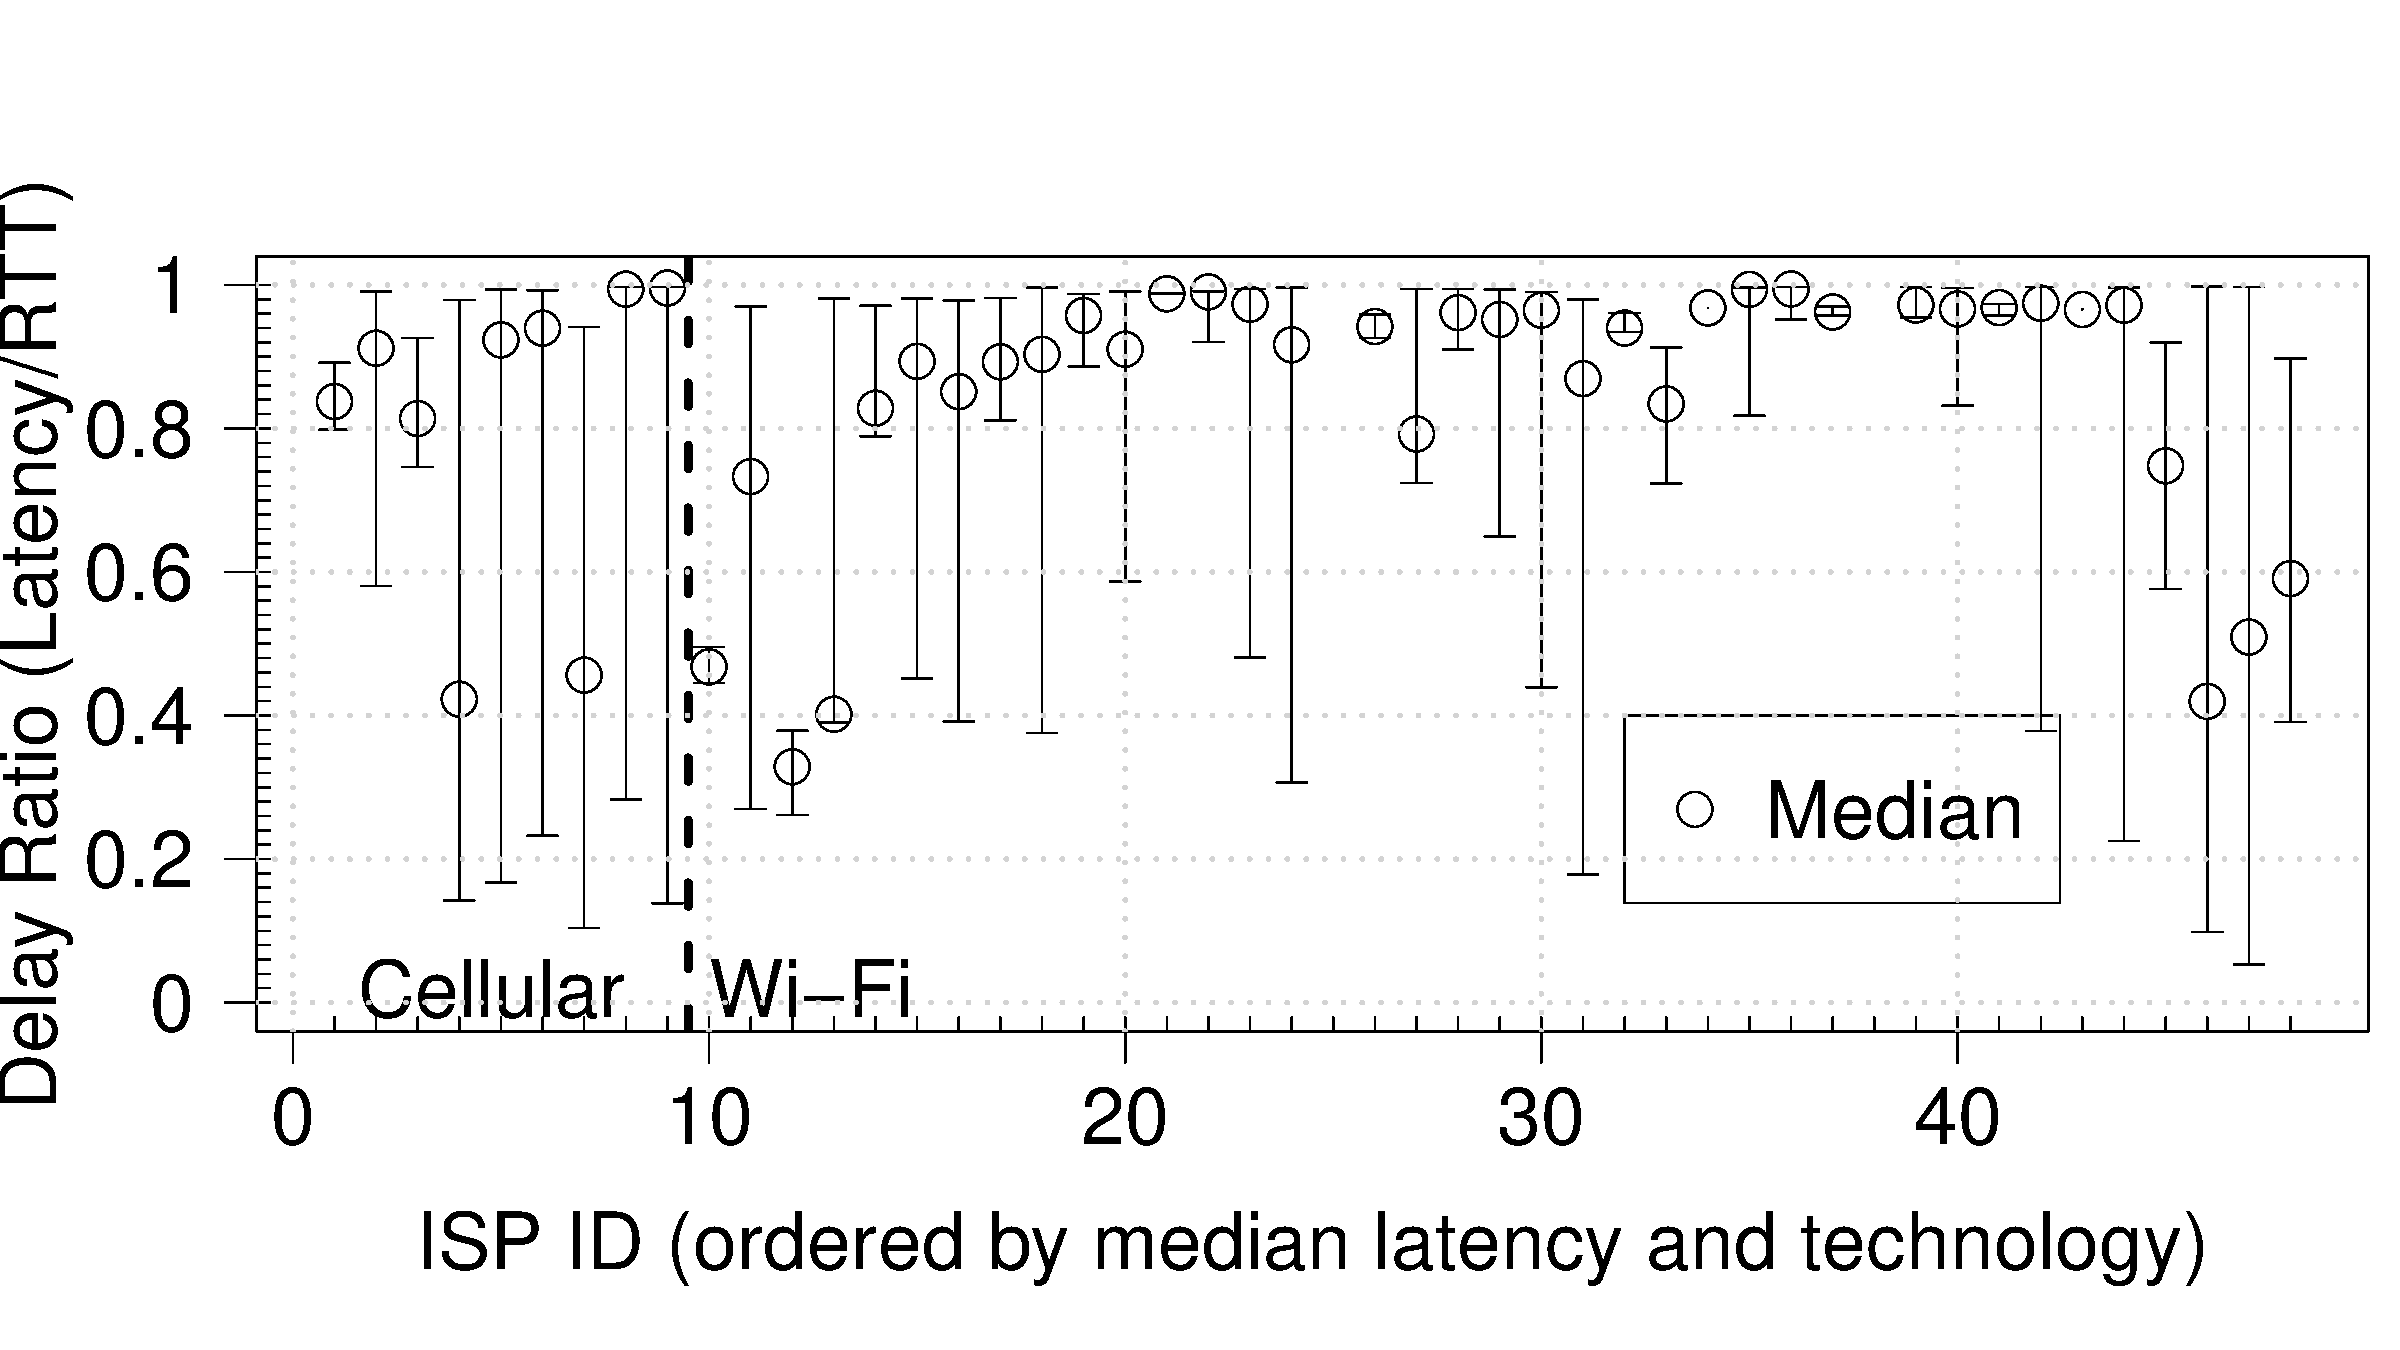
\includegraphics[width=\columnwidth]{plots/delay_ratio_isp_whisker.pdf}
\caption{Latency as a fraction of the round trip time to contact google services. \emph{In 35 ISPs of the 48 ISPs we observe that the latency of the mobile device to our server accounts for more than 90\% of the end-to-end round trip time. Error bars indicate the 91st and 9th percentile.}}
\label{fig:compare-delay-ratio}
\end{figure}

\begin{figure}[t]
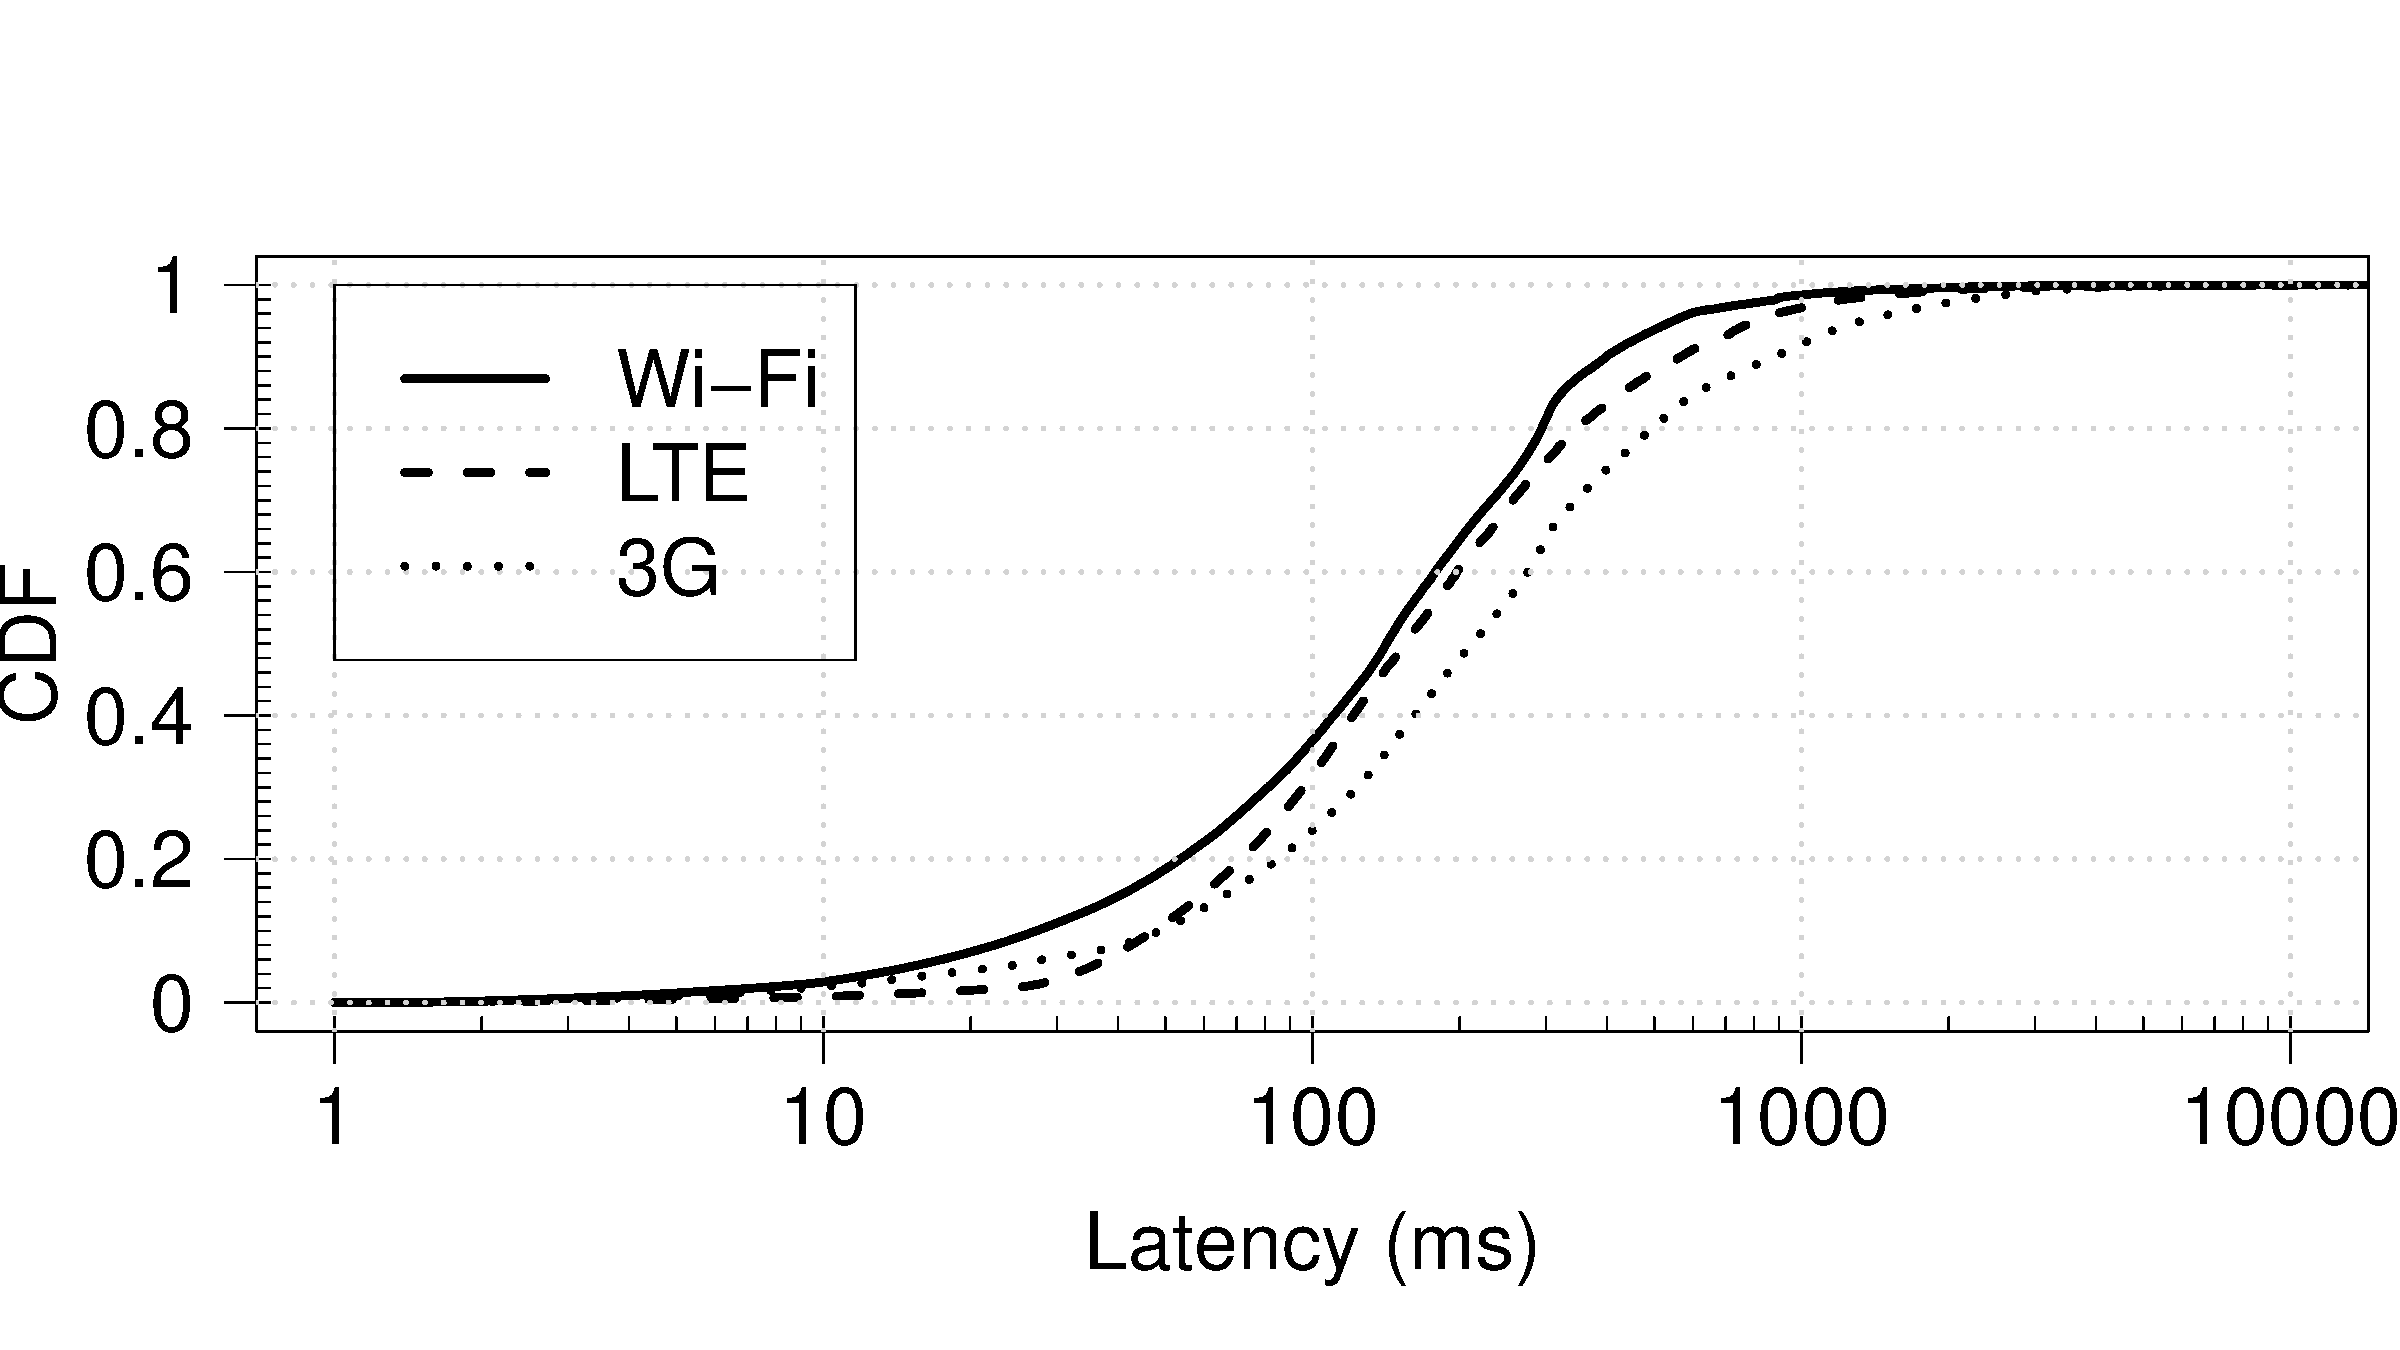
\includegraphics[width=\columnwidth]{plots/distrib_latency_technology.pdf}
\caption{Distribution of latency over cellular and \wifi ISPs. \emph{The distribution of latency observed when using LTE in the wild is similar to that observed for \wifi}.}
\label{fig:compare-delay-ratio}
\end{figure}

\begin{figure}[t]
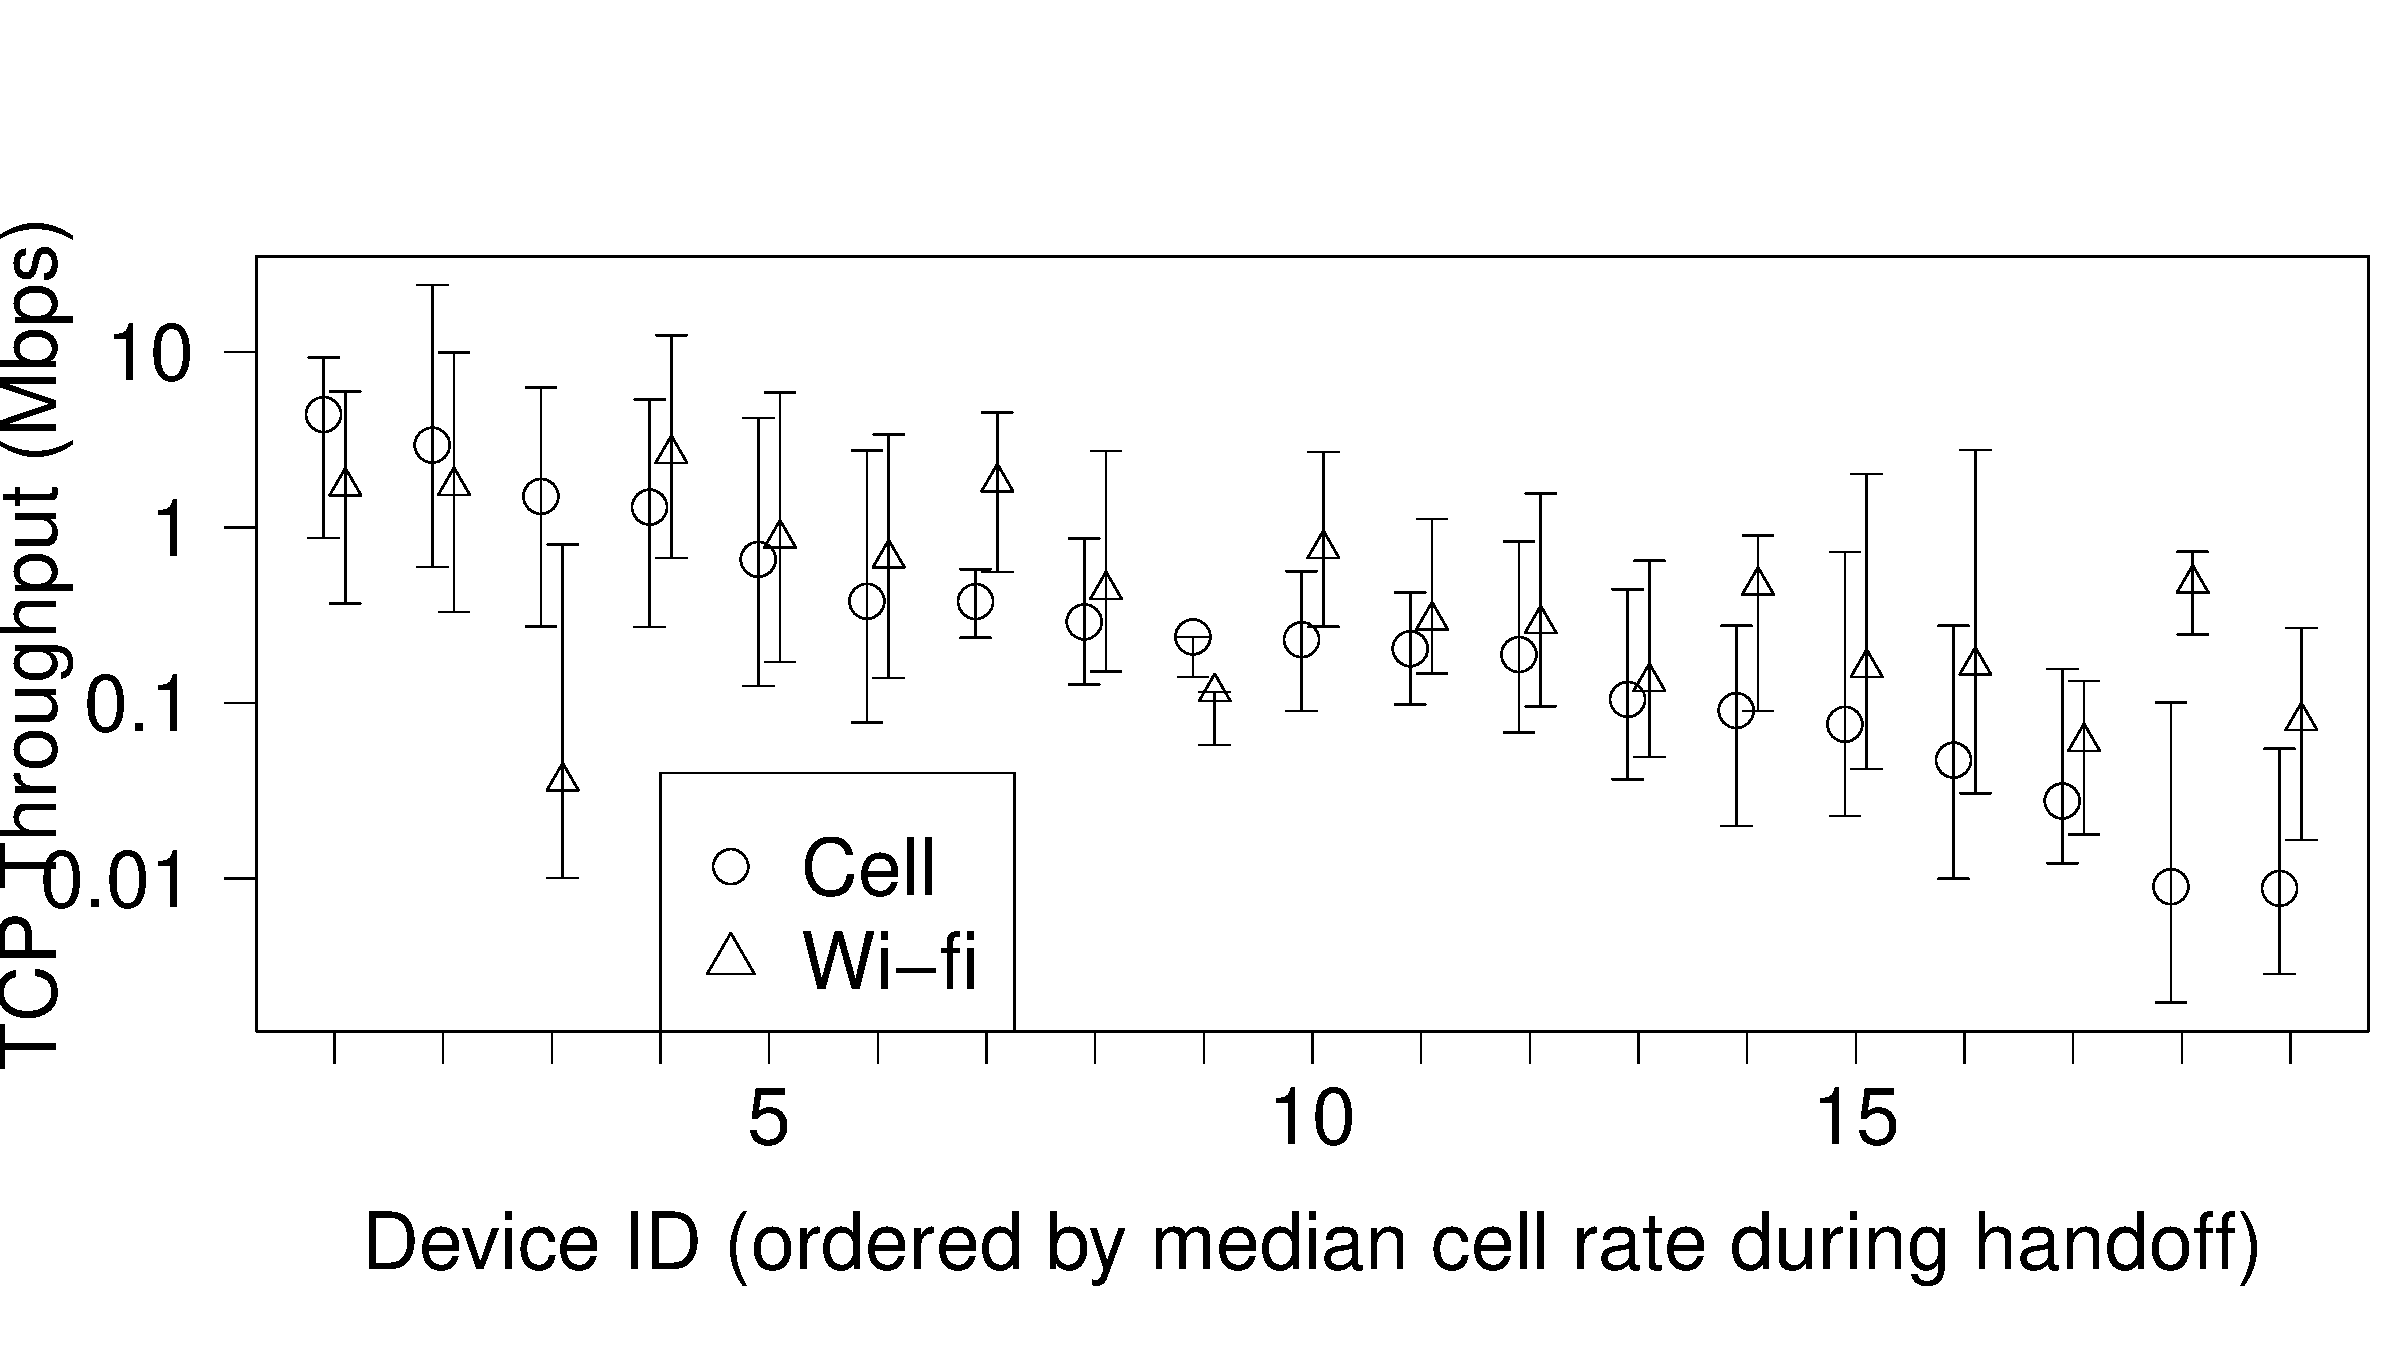
\includegraphics[width=\columnwidth]{plots/handoff_rates.pdf}
\caption{TCP Throughput observed during the hour of the handoff. \emph{The three users that have LTE connections observed a better TCP throughput over LTE in comparison to \wifi in the hour of the handoff. Error bars indicate the 91st and 9th percentile}.}
\label{fig:compare-handoff}
\end{figure}




\tbd{We performed a traceroute from our server to the egress link and found }



\section{Related Work}
\label{sec:related}

The network behavior of mobile systems has implications for battery life, 
data-plan consumption, privacy, security and performance, among others. 
When attempting to characterize this behavior, researchers face a number 
of trade-offs: compromising network coverage (limiting the number and type of ISPs measured), 
portability (limiting the device OSes) and/or deployability (limiting subscriber coverage).
\platname compromises 
none of these, enabling comprehensive measurements across carriers, devices and access 
technologies. Table~\ref{tab:relatedCompare} puts our approach in context with previous 
approaches for measuring the network behavior of mobile systems. 

\begin{table*}[t]
\begin{center}
{\footnotesize
\begin{tabular}{|l|l|l|l|l|}
\hline
 & \textbf{Network Coverage} &  \textbf{Portability} &  \textbf{Deployment model} &   \textbf{Meas. Type}  \\ \hline
AT\&T/Telefonica study~\cite{vallina-rod:ads,gerber:passivespeed} & Single carrier & All OSes & Instrument cell infrastructure & Passive \\ \hline
WiFi study~\cite{chen:wifi} & Single WiFi network & All OSes & Instrument WiFi network & Passive \\ \hline
PhoneLab/TaintDroid~\cite{enck:taintdroid} & Multiple networks & Android & Install custom OS & Active/Passive \\ \hline
MobiPerf~\cite{wang:middleboxes}/SpeedTest~\cite{sommers:cellwifi} & Multiple networks & Android & Install App & Active \\ \hline
\platname & Any network & Android / iOS & VPN configuration & Passive \\ \hline
\end{tabular} }
\end{center}
\label{tab:relatedCompare}
\caption{Comparison of alternative measurement approaches. \platname is the first approach to cover all access networks and most device OSes, capturing 
network traffic passively and with low overhead via VPN proxying.}
\end{table*}%

Traces from mobile devices can inform a number of interesting analyses. Previous work 
uses custom OSes to investigate how devices waste energy~\cite{pathak:eprof}, network bandwidth and 
leak private information~\cite{enck:taintdroid,hornyack:appfence}. Similarly, AppInsight~\cite{ravindranath:appinsight} and PiOS~\cite{egele:pios} can inform 
app performance through binary instrumentation and/or static analysis. In this work, we explore the opportunity to use network traces 
alone to reveal these cases without requiring any OS or app modifications.

Network traces from inside carrier networks provide a detailed view for large numbers 
of subscribes. For example, Vallina-Rodriguez~\etal~\cite{vallina-rod:ads} uses this approach to characterize performance and 
the impact of advertising. Gerber \etal~\cite{gerber:passivespeed} similarly use this approach to 
estimate network performance for mobile devices.  \cite{maier:mobtraffic} \cite{chen:wifi}
Similar to these approaches, \platname provides continuous passive monitoring of mobile network 
traffic; however, \platname is the first to do so across all networks to which a device connects.

Last, active measurements~\cite{wang:middleboxes,sommers:cellwifi} allow researchers to understand network topologies and instantaneous 
performance at the cost of additional, synthetic traffic for probing. In contrast, \platname uses 
passive measurements to characterize the traffic that devices
naturally generate.

%%% Local Variables: 
%%% mode: latex
%%% TeX-master: "main.tex"
%%% End: 


\section{Conclusion}
\label{sec:conclusion}

This paper described how we use proxying to provide a comprehensive view of Internet traffic 
generated by mobile devices. The key observation is that most devices already support traffic 
indirection via VPNs; by using VPN servers as proxying and instrumenting them to record 
traffic flows, we passively monitor traffic from mobile devices regardless of access 
technology, device or OS. Using this unique view of mobile-device traffic, we conduct 
controlled experiments and user studies to characterize and classify apps and to identify 
PII leakage. As part of future work, we are investigating additional 
techniques to improve traffic classification and to identify PII. To understand network 
behavior from a much more diverse set of users and devices, we are deploying 
a second study that is IRB-approved for a larger set of users without requiring 
in-person interviews. 

%\section{Classification Methodology}
\label{sec:classification-methodology}

\platname offers a network perspective of the mobile Internet traffic.
To detail the mobile traffic, we need to first identify the access technology used by the devices, and the applications and Web-services responsible for each flow captured by \platname.
In this section we describe the technique we used to identify the access technology and the applications and Web-services. 

\subsection{Access Technology Classification}

To quantify the impact of the access technology, we need to first identify the access technology used by the devices when accessing the Internet via \platname servers.
A mobile devices can access the Internet using either \wifi or cellular networks. 
We estimate the access technology with the description of the AS through which the mobile client connects to our \platname server. 
We get this AS description by performing a \emph{WHOIS} lookup on the IP address used by the mobile client to tunnel Internet traffic. 
For our analysis, we use the WHOIS databases available at \emph{whois.cmyru.com} and \emph{utrace.de}.
We use the information from these \emph{WHOIS} databases to manually classify the ASes to be either cellular or \wifi.
Our dataset consists of data traffic from 54 distinct ASes, of which we classify 9 to belong to cellular networks.
Each device connected our \platname server from at most two distinct ASes during the measurement study.
In contrast, a median of 4 \wifi ASes were observed per device and for one device we observed traffic from 25 different \wifi ASes that were spread across 5 countries. 

\subsection{Classification of Mobile Applications and Services}

The data traffic from mobile devices is because of the applications running on the device and OS services and libraries used by the applications. 
To analyze the behavior of mobile services we need to first associate the observed flows with the applications and the OS services responsible for the flows.
For our analysis, we focus on identifying the OS services and the applications and Web-services responsible for HTTP and SSL flows, the largest sources of mobile Internet traffic~\cite{maier:mobtraffic,falaki:mobileusage,xu:appusage}.

\begin{table}
\begin{small}
\begin{center}
\begin{tabular}{|p{0.15\columnwidth}|p{0.12\columnwidth}|r|r|r|r|}
\hline
\multirow{2}{*}{\bf IP Protocol} & \multirow{2}{*}{\bf Service} & \multicolumn{2}{|c|}{\bf Android} & \multicolumn{2}{|c|}{\bf iOS} \tabularnewline
\cline{3-6}
           &           &  \textbf{Cell.}  &  \textbf{\wifi}  &  \textbf{Cell.}  &  \textbf{\wifi}  \tabularnewline
\hline
\multirow{3}{*}{TCP}
       &  HTTP  & 35.386 & 68.686 & 52.109 & 75.506 \tabularnewline
\cline{2-6}
       &  SSL   & 61.135 & 27.366 & 46.765 & 18.777 \tabularnewline
\cline{2-6}
       &  other & 2.346  & 3.290  & 0.256  & 1.818 \tabularnewline
\hline
\multirow{2}{*}{UDP}
       &  DNS   & 0.682  & 0.496  & 0.545  & 0.305  \tabularnewline
\cline{2-6}
       &  other & 0.316  & 0.098  & 0.286  & 3.583  \tabularnewline
\hline
 Other &  -     & 0.135  & 0.064 & 0.039  & 0.011  \tabularnewline
\hline
\multicolumn{2}{|c|}{\emph{total}} & 100.00 & 100.00 & 100.00 & 100.00 \tabularnewline
\hline
\end{tabular}
\end{center}
\end{small}
\caption{Traffic volume (in percentage) of popular protocols and services on Android and iOS devices over cellular and \wifi.
\emph{TCP flows are responsible for more than 90\% of traffic volume. Traffic share of SSL over cellular networks is more than twice the traffic share of SSL over \wifi.}} 
\label{tab:summaryIOSAndroidTraffic}
\end{table}

We begin our identification process using the classification provided Bro~\cite{bro}.
Bro uses the protocol field in the IP header to broadly classify the flows, and we use this classification to label flows as either TCP, UDP, or \emph{other}.
Bro further classifies TCP flows using well defined port numbers, and we use this classification to label flows as either HTTP, SSL (which includes HTTPS, IMAP, etc.) or \emph{other} flows.
Similarly, we use Bro to label UDP flows as either DNS or \emph{other}. 
Indeed, in \fref{tab:summaryIOSAndroidTraffic}, we observe that more than 92\% of the traffic in our \mobWild dataset is either HTTP or SSL. 
We also observe that the share of HTTP volume over \wifi and ce
llular are significantly different. 
This increase is a result of the reduced share of media traffic and the use of email and for social networking applications that rely on SSL.

\subsubsection{HTTP Traffic Classification}

Differences with ~\cite{erman2011http,xu:appusage,maier:mobtraffic}.

Web-services rely on the \useragent field to distinguish HTTP flows from their mobile applications from the flows originating from Web-browsers.
In our controlled experiments we observed a valid \useragent string in more than 99\% of the HTTP flows from Android and iOS.
However, because the mobile applications use built in OS services and libraries to download media content, we do not observe the identifier of the application using the OS service and library in the \useragent string for media traffic. 
For example, when an iOS devices is used to stream YouTube video on a YouTube Application or if the video is viewed on clicking a video link on Facebook application, we observe that the media content is downloaded by AppleCoreMedia service of iOS~\cite{apple:coremedia}. 
We now show how a combination of \useragent and \httphost can be used to identify either the Web-service or the application associated with the flow.

\begin{figure}
\subfloat[iOS]{\label{fig:http-wordcloud-ios}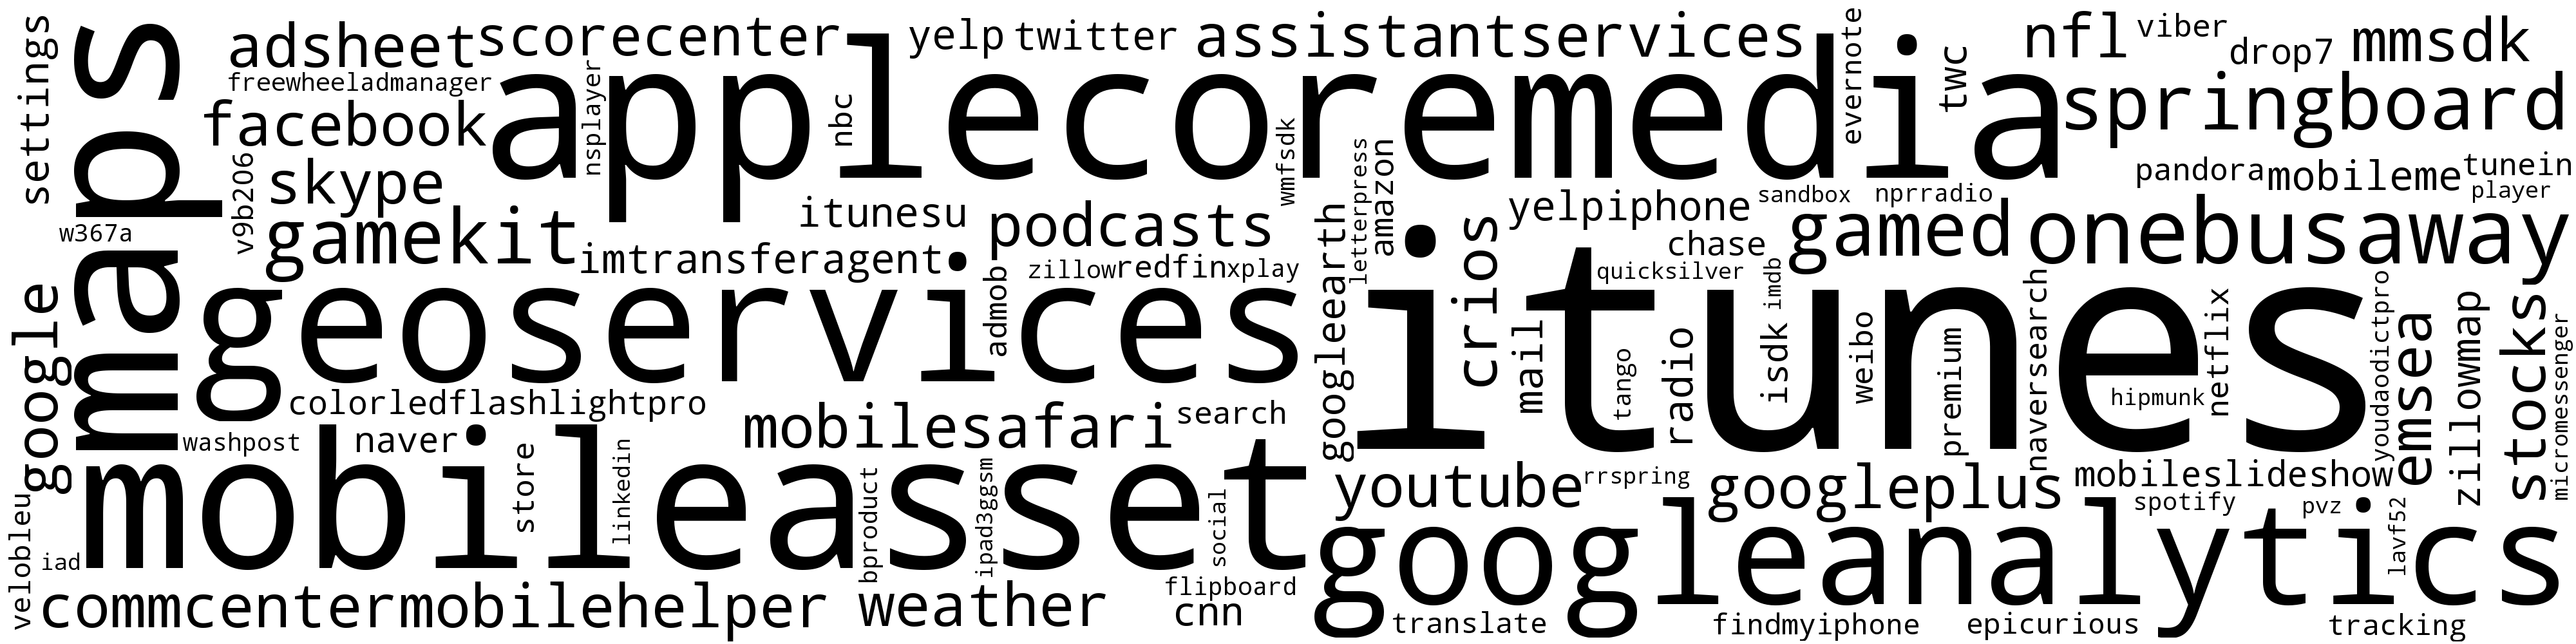
\includegraphics[width=\columnwidth]{figures/wordcloud_useragentsignature_ios_image.png}}\newline
\subfloat[Android]{\label{fig:http-wordcloud-android}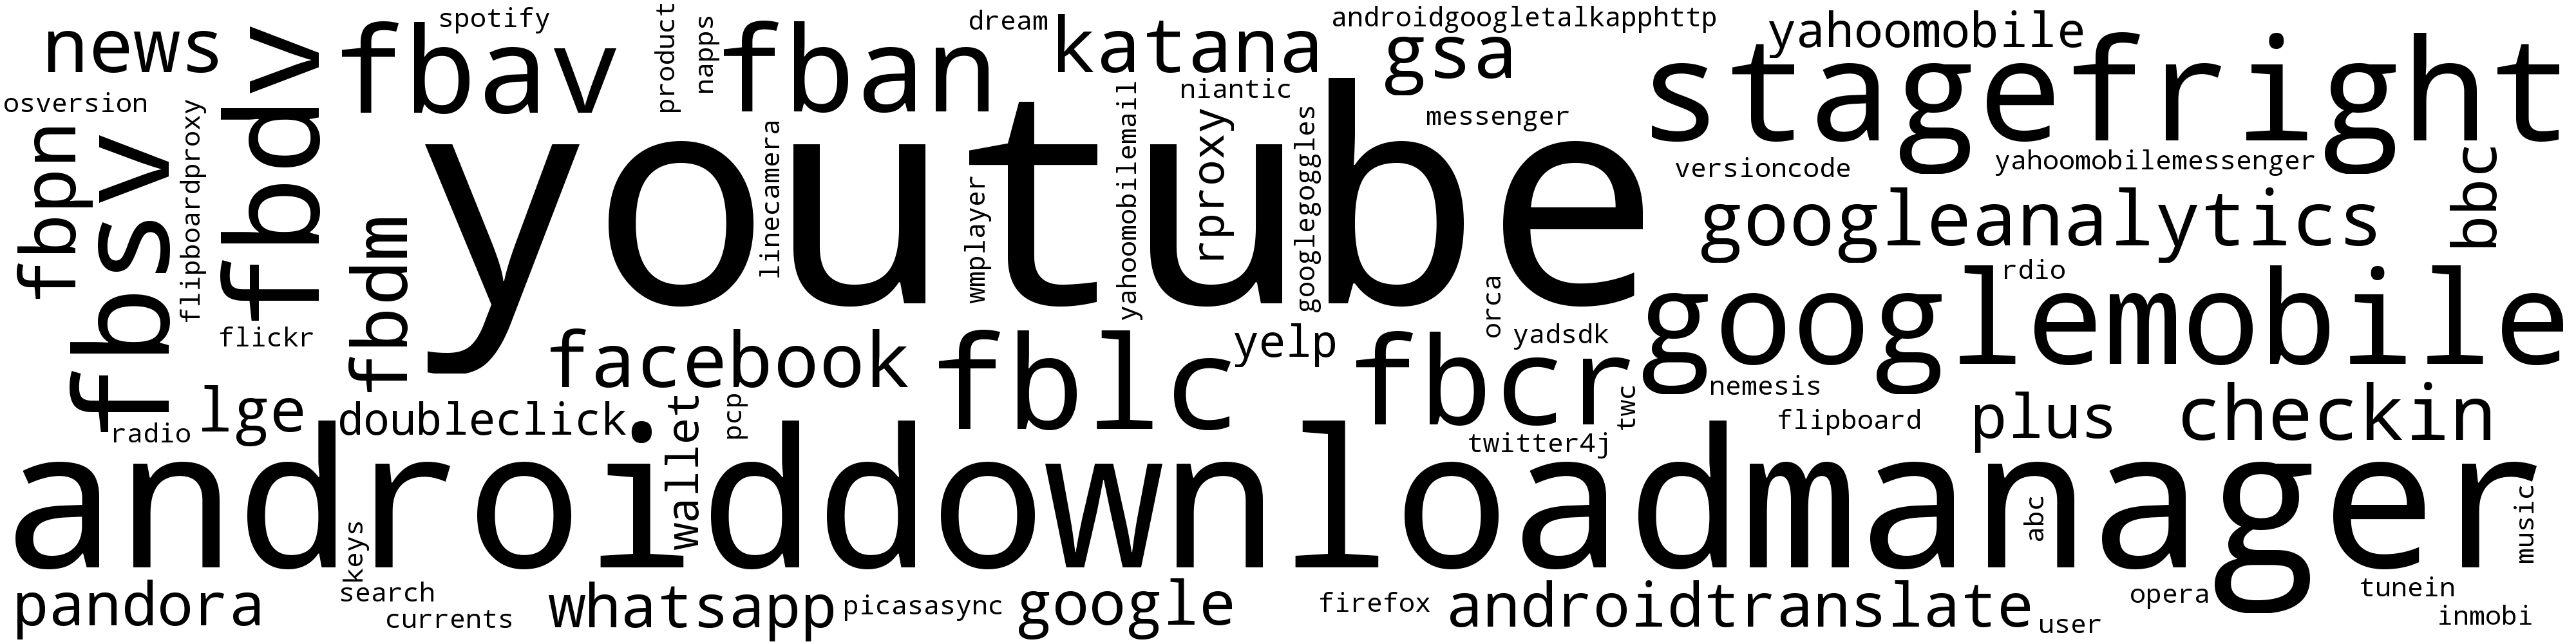
\includegraphics[width=\columnwidth]{figures/wordcloud_useragentsignature_android_image.png}}
\caption{\useragent signatures in  iOS and Android HTTP flows. \emph{The font weight represents the number of users for which a particular signature was observed.}}
\label{fig:http-wordcloud}
\end{figure}

We observe that more than 98\% of HTTP traffic from Android and iOS devices in the \mobWild dataset have a valid \useragent string; we observe a total of 1435 unique \useragent strings across Android and iOS devices. 
These \useragent strings contain an application identifier and other auxiliary information such as details of the OS, manufacturer, display resolutions, carrier, and information such as versions and compatibility with other browser engines~\cite{mozilla:useragentdetection}. 
We use regular expression to extract the tokens that contain the application information, and cluster these tokens using edit distance\footnote{We plan to release this code along with \platname package.}.
At the end of this process we were able to identify 361 unique signatures which we resolve as either applications or OS services. 

In \fref{fig:http-wordcloud} we present a \emph{word cloud} of the signatures we were able to extract from \useragent field; the text size of the signature represents the number of users for which the signature was observed.
Despite the usefulness of the \useragent, we observe that relying only on the \useragent is not sufficient to identify the application.
For example, we observe the signatures \emph{applecoremedia} and \emph{stagefright} in the \emph{word cloud} for iOS devices and Android devices, signatures of the OS services responsible to download media content.

The iOS devices rely on AppleCoreMedia service~\cite{apple:coremedia} to download media content.
We therefore observed the signature of AppleCoreMedia in more than 98.45\% of the content downloaded from the YouTube servers (which we identify based on the \httphost field in the \httpget requests). 
Similarly, depending the Android version we observe either the signature for Stagefright\cite{android:stagefright} or no application or OS service signature for YouTube traffic to Android devices. 
Indeed, we observed signatures for popular media services such as Netflix, YouTube, Vimeo, Pandora, etc. in the \httphost field in the majority traffic from iOS devices and Android devices. 
We therefore used the \httphost field to classify media content.

\begin{table}
\centering
\begin{small}
\begin{tabular}{|p{0.25\columnwidth}|c|c|c|c|}
\hline
\multirow{2}{*}{\bf Category} & \multicolumn{2}{c|}{\bf iOS} &  \multicolumn{2}{c|}{\bf Android} \tabularnewline
\cline{2-5}
  & {\bf Bytes}  & {\bf Flows} & {\bf Bytes} & {\bf Flows}   \tabularnewline
\hline
Media (Popular)         & 51.405  & 12.131 & 65.922 & 22.377 \tabularnewline
\hline
Application             & 33.987  & 80.758 & 31.353 & 77.498 \tabularnewline
\hline
Media (Other)       & 14.572  &  5.914 &  2.712 &  0.044 \tabularnewline
\hline
Other                   &  0.036  & 1.1963 &  0.013 &  0.081 \tabularnewline
\hline
{\em total}            & 100 & 100 & 100 & 100 \tabularnewline
\hline
\end{tabular}
\end{small}
\caption{Classification of HTTP Traffic.}
\label{tab:classify-http}
\end{table}

In summary, we use a combination of \useragent and \httphost field in HTTP headers to classify HTTP traffic.
In \fref{tab:classify-http}, a table that provides an overview of our classification results.
We observe that we were able to classify more than 98\% of the traffic in terms of flows and bytes from iOS and Android devices using the \useragent and the \httphost field. 
We observe that media from popular hosts contribute to more than 50\% of the traffic volume from iOS and Android devices.
Similarly, we were able to identify applications for more than 77\% of flows from Android and iOS devices. 
However, we observe media (identified based on the \useragent) served from CDNs and others hosts from which we could not identify the webservice from other fields in the HTTP header and the DNS responses before the HTTP flows to be 14.5\% of the traffic volume for the iOS devices in our dataset.

\subsubsection{Classification of SSL Traffic.}

Unlike HTTP flows, SSL flows provide limited information that can be used to identify the applications. 
Our objective classifying SSL traffic was therefore focused towards identifying the Web-services responsible for the SSL flows. 
We now show how we used the port number, the SSL certificate with server name identification, and DNS queries to identify the source of SSL traffic. 

\begin{table}
\centering
\begin{small}
\begin{tabular}{|p{0.25\columnwidth}|c|c|c|c|}
\hline
\multirow{2}{*}{\bf Service} & \multicolumn{2}{c|}{\bf iOS} &  \multicolumn{2}{c|}{\bf Android} \tabularnewline
\cline{2-5}
  & {\bf Bytes}  & {\bf Flows} & {\bf Bytes} & {\bf Flows} \tabularnewline
\hline
HTTPS                   & 91.287 & 81.960 & 97.852 & 97.168    \tabularnewline
\hline
Mail                    &  6.700 & 15.872 & 0.689  & 0.320  \tabularnewline
\hline
Notification            &  1.412 & 1.553  & 1.321  & 2.100  \tabularnewline
\hline
Other                   &  0.601 & 0.615  & 0.138  & 0.412 \tabularnewline
\hline
{\em total}             & 100 & 100 & 100 & 100 \tabularnewline
\hline
\end{tabular}
\end{small}
\caption{Classification of SSL Traffic based on port number. \emph{HTTPs is the most popular service that uses SSL in the \mobWild dataset.}}
\label{tab:classify-ssl-port}
\end{table}

Mobile devices use SSL for various services including mail, notifications, instant messaging, and web browsing.
Services such as mail, instant messaging, and notifications are documented to use dedicated port numbers of their traffic\footnote{We also use the AS for identifying the notification messages as detailed in \fref{sec:characterize-os}.}
On using port numbers, we observe in \fref{tab:classify-ssl-port} that a majority of SSL traffic by volume and flows is HTTPS.
We then focus our attention on indentifying the Web-services responsible for the HTTPs flows. 

We first use the common name (CN) field of certificates to identify the servers that exchanged data using HTTPS.
We observe that less than 25\% of the HTTPS traffic from iOS and Android contains the fully qualified domain name (FQDN) in the subject of the certificate; the rest of the traffic either contains regular expressions such as *.google.com in the certificate or is a continuation of a previous SSL session. 
To further resolve the hostnames, we rely on \emph{server name indication} used by SSL flows~\cite{rfc:servernametls}.
Servers that host multiple services use the \emph{server name indication} to distinguish these services.   
For example, we observe a \emph{server name indication} of \emph{plus.google.com} and \emph{s.youtube.com} in two flows that used a certificate with a CN \emph{*.google.com}.
However, we observe that by using either the certificate or the \emph{server name} we were able to identify the name of the Web-service in less than \tbd{40}\% of iOS and Android HTTPS traffic.

For such flows we use DNS requests made by the mobile devices before starting the HTTPS flows, a technique similar to DN-Hunter~\cite{bermudez:dnhunter}.
DN-Hunter relies on the most recent FQDN that corresponds to the IP address, however in our controlled experiments we observe Android and iOS devices use the first entry in DNS response while resolving \emph{hostnames}.
We therefore use the latest DNS response that contains the IP address of the webservice in the first position of the DNS response. 
Indeed, for 97.8\% of the Android and 83.4\% of the iOS HTTPS traffic that we could not classify using other fields, we observe that the latest DNS response before the flow started contained the IP address of the webservice as the first entry in the DNS response\footnote{The share of SSL traffic where the latest DNS response contains the IP address of the web-service in the first position is 97.4\% for Android and 88.6\% of iOS}. 
Despite the potential usefulness of DNS responses, we give a high priority to the server-name and the certificates because we observed that for flows that contained the server name did not contain the same name in the DNS response for 9.2\% of the iOS traffic and 5.6\% of Android traffic.

\begin{table}
\centering
\begin{small}
\begin{tabular}{|c|c|}
\hline
{\bf iOS} & {\bf Android} \tabularnewline
\hline
imap.gmail.com & picasaweb.google.com \tabularnewline
www.google.com & www.googleapis.com \tabularnewline
sphotos-a.xx.fbcdn.net & android.clients.google.com \tabularnewline
itunes.apple.com  & clients4.google.com \tabularnewline
m.google.com & fbcdn-photos-a.akamaihd.net \tabularnewline
\hline
\end{tabular}
\end{small}
\caption{Popular hostnames for iOS and Android based on traffic volume.}
\label{tab:sslclassify-popular-host}
\end{table}

In \fref{tab:sslclassify-popular-host} we present the top5 hostnames that were responsible for 66\% of iOS traffic and 54\% of Android by volume. 
We observe that despite the hostname we cannot uniquely identify the application. 
For example, \emph{www.google-apis.com} and \emph{clients4.google.com} offer limited information on the application or web-service that is responsible for the content; one can only guess that these flows belong to some google service.
However, hostname such as \emph{fbcdn-photos-a.akamaihd.net} gives an indication that the traffic is due to facebook.

\begin{table}
\centering
\begin{small}
\begin{tabular}{|p{0.35\columnwidth}|c|c|c|c|}
\hline
\multirow{2}{*}{\bf Service} & \multicolumn{2}{c|}{\bf iOS} &  \multicolumn{2}{c|}{\bf Android} \tabularnewline
\cline{2-5}
  & {\bf Bytes}  & {\bf Flows} & {\bf Bytes} & {\bf Flows} \tabularnewline
\hline
Mail                 & 9.970    & 62.168   & 1.626  & 1.565 \tabularnewline
\hline
Social Networking    & 12.491   & 6.683    & 36.661 & 22.352 \tabularnewline
\hline
Apple/Google Store   & 5.457    & 3.463    & 0.044  & 0.036 \tabularnewline
\hline
Instant Messages     & 0.982    & 7.089    & 1.411  & 3.109 \tabularnewline
\hline
Other Google Services & 58.665   & 13.32510 & 45.024 & 46.089 \tabularnewline
\hline
\emph{total}         & 87.564   & 92.728   & 84.776 & 73.151 \tabularnewline
\hline
\end{tabular} 
\end{small}
\caption{Sample classification of SSL traffic based on names in certificate, server name identification, and DNS request.}
\label{tab:classify-ssl-traffic}
\end{table}

In \fref{tab:classify-ssl-traffic} we show how we grouped SSL traffic based on names identified using the SSL fields and DNS queries and port numbers.
We observe that the iOS devices in our dataset generated a significant number of flows to email sites.
Similarly, we were able to group 12.49\% of iOS and 36.661\% of Android traffic with social network services that includes \emph{Google Plus, Facebook, and Twitter}.
We speculate the increase in traffic share for Android devices is because Android devices offer services to backup photos on \emph{Google Plus}.
Similarly, we observe that 5.4\% of the traffic from iOS devices was from Apple stores while we observe only 0.04\% of traffic to the \emph{Google Play} store. 
This low share is because google can use hosts matching the pattern \emph{client*.google.com} to serve for different Web-services.
We observed a similar behavior in our controlled experiments, and we group such traffic as \emph{other google services}.
Indeed, in \fref{tab:classify-ssl-traffic} we observe that traffic from Google is the largest source of SSL traffic for iOS and Android devices in our dataset. 

In summary, we use \platname to perform controlled experiments and in the wild measurements to characterize mobile Internet traffic. 
We use Bro to analyze the data and build on the output of bro to further classify HTTP flows and SSL flows to identify the source of the traffic. 
We now present the results of our experiments and measurements study. 


%%% Local Variables: 
%%% mode: latex
%%% TeX-master: "main.tex"
%%% End: 

% Popular webservices such as google are known to use the same pool of IP addresses for various applications, for example the IP for gmail may also be used for search. 
% In \fref{fig:ssl-classification-app-service} we present the fraction of SSL traffic where the most recent DNS response contained the IP address of the SSL flow in the first position. 
% We observe that for the majority of SSL traffic by volume and flows can be classified by using the DNS responses. 

% \begin{table}
% \centering
% \begin{small}
% \begin{tabular}{|p{0.35\columnwidth}|c|c|c|c|}
% \hline
% \multirow{2}{*}{\bf Service} & \multicolumn{2}{c|}{\bf iOS} &  \multicolumn{2}{c|}{\bf Android} \tabularnewline
% \cline{2-5}
%   & {\bf Bytes}  & {\bf Flows} & {\bf Bytes} & {\bf Flows} \tabularnewline
% \hline
% FQDN in Certificate    & 24.274 & 31.423  & 19.318 & 29.424 \tabularnewline
% \hline
% Regular expression     & 50.463 & 35.318  & 42.427 & 31.670 \tabularnewline
% \hline
% No Subject or CN       & 25.263 & 33.259  & 38.254 & 38.906 \tabularnewline
% \hline
% {\em total}            & 100 & 100 & 100 & 100 \tabularnewline
% \hline
% \end{tabular}
% \end{small}
% \caption{Classification of HTTPs based on certificates.}
% \label{tab:classify-http-cert}
% \end{table}
%\section{Application Characterization}
\label{sec:characterize-app}

  We now turn to measurements of specific popular iOS and Android applications. 
  When users install apps, they grant them Internet access without detailed knowledge of how that access will be used, including {\it how much} data is sent or accessed, {\it what} data is sent,  or {\it with whom} the app communications.
  ``How much'' is important to conserve both bandwidth caps and battery capacity: an app which consumes or produces too much data will waste bandwidth resources, while an app which consumes or produces data too frequently will prevent the device radio from going idle to save power.
  ``With whom'' is important to protect users from excessive tracking -- the more organization's servers an app connects to, the more organizations which are able to track user behavior, location, or other private data.
  Finally, ``what data'' is important because apps may unnecessarily leak personally identifiable information (PII) such as user email address, IMEI, contact information, or other stored data either to the app provider or worse, to any eavesdropper on a public WiFi connection.
  We  report on our findings in all three of these dimensions for the iPhone and Android apps in our study.

\subsection{Bandwidth and Radio Usage}

  {\bf In the Wild.}
    \begin{itemize}
      \item Stats on how much bandwidth each user used; time of day; how frequent...
    \end{itemize}

  {\bf Android Apps.}
    To dig in to the root cause of these usage patterns, we also did an `app-by-app` analysis of network usage to see if most bandwidth consumption/radio time was the result of a few heavy applications, with most applications relatively idle, or whether usage was divided amongst all applications equally.
    In Figure~\ref{fig:app-by-app-usage}, we plot the CDF of total bytes transferred by each app in our study, one line for the top-100 Google Play apps we tested manually, and another for the top 2000 apps, tested automatically, from a third-party market.
    We see that...\tbd{Amy...}
    Regarding radio usage,...\tbd{Do we even have time to do this? I don't remember the exact metrics we used for the MobiSys submission.}

  {\bf iPhone Apps.}

\subsection{Third Party Servers}
  Many free applications support themselves financially by serving ads or providing resources for third parties to track user behavior.
  We now explore how many servers are contacted by a given app (\ie{} how many providers are tracking a user with this app) -- most of these typically for ads, tracking, or analytics -- as well as how much data is transferred to and from these servers (\ie{} how much does this traffic impact the user's data cap?).

  {\bf In the Wild.}
  We first consider the overall impact of these ads, analytic, and tracking services on typical user behavior in our IRB study...
  \tbd{Ashwin...}

\begin{figure}[t]
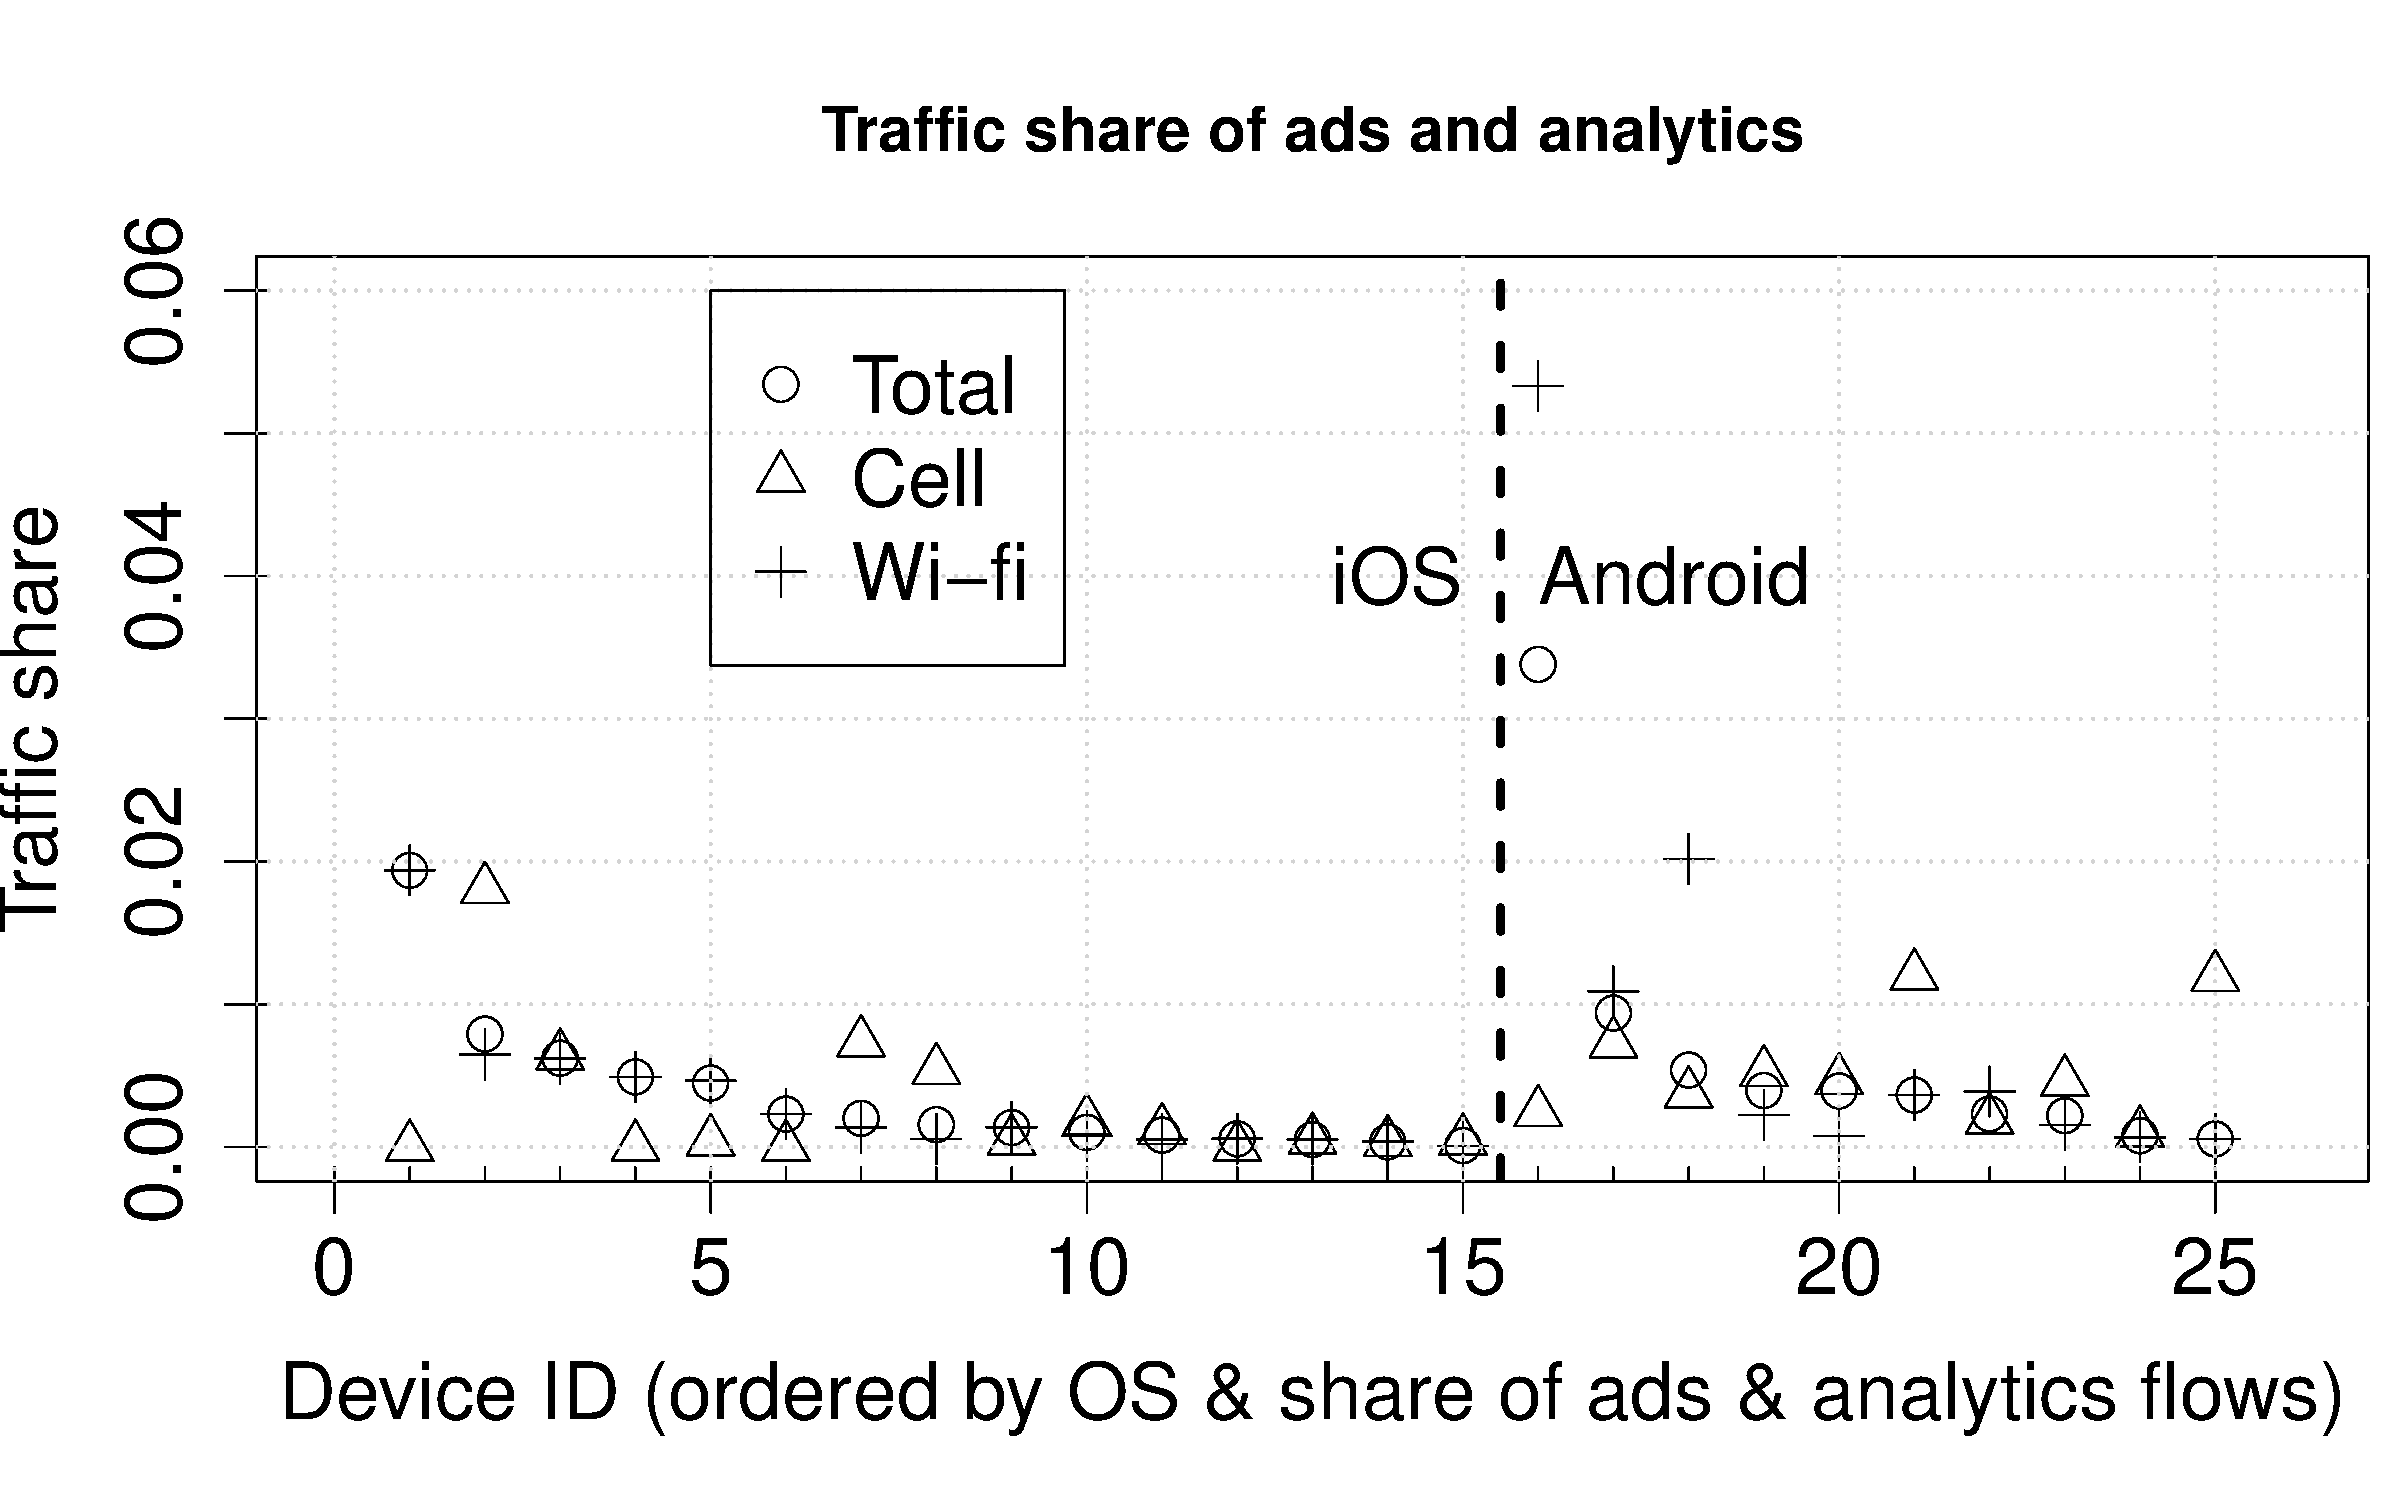
\includegraphics[width=\columnwidth]{plots/ad_share_bytes.pdf}
\caption{Fraction of traffic volume because of Ads and Analytics. \emph{\tbd{Check for id1 and id25}}}
\label{fig:description}
\end{figure}

\begin{figure}[t]
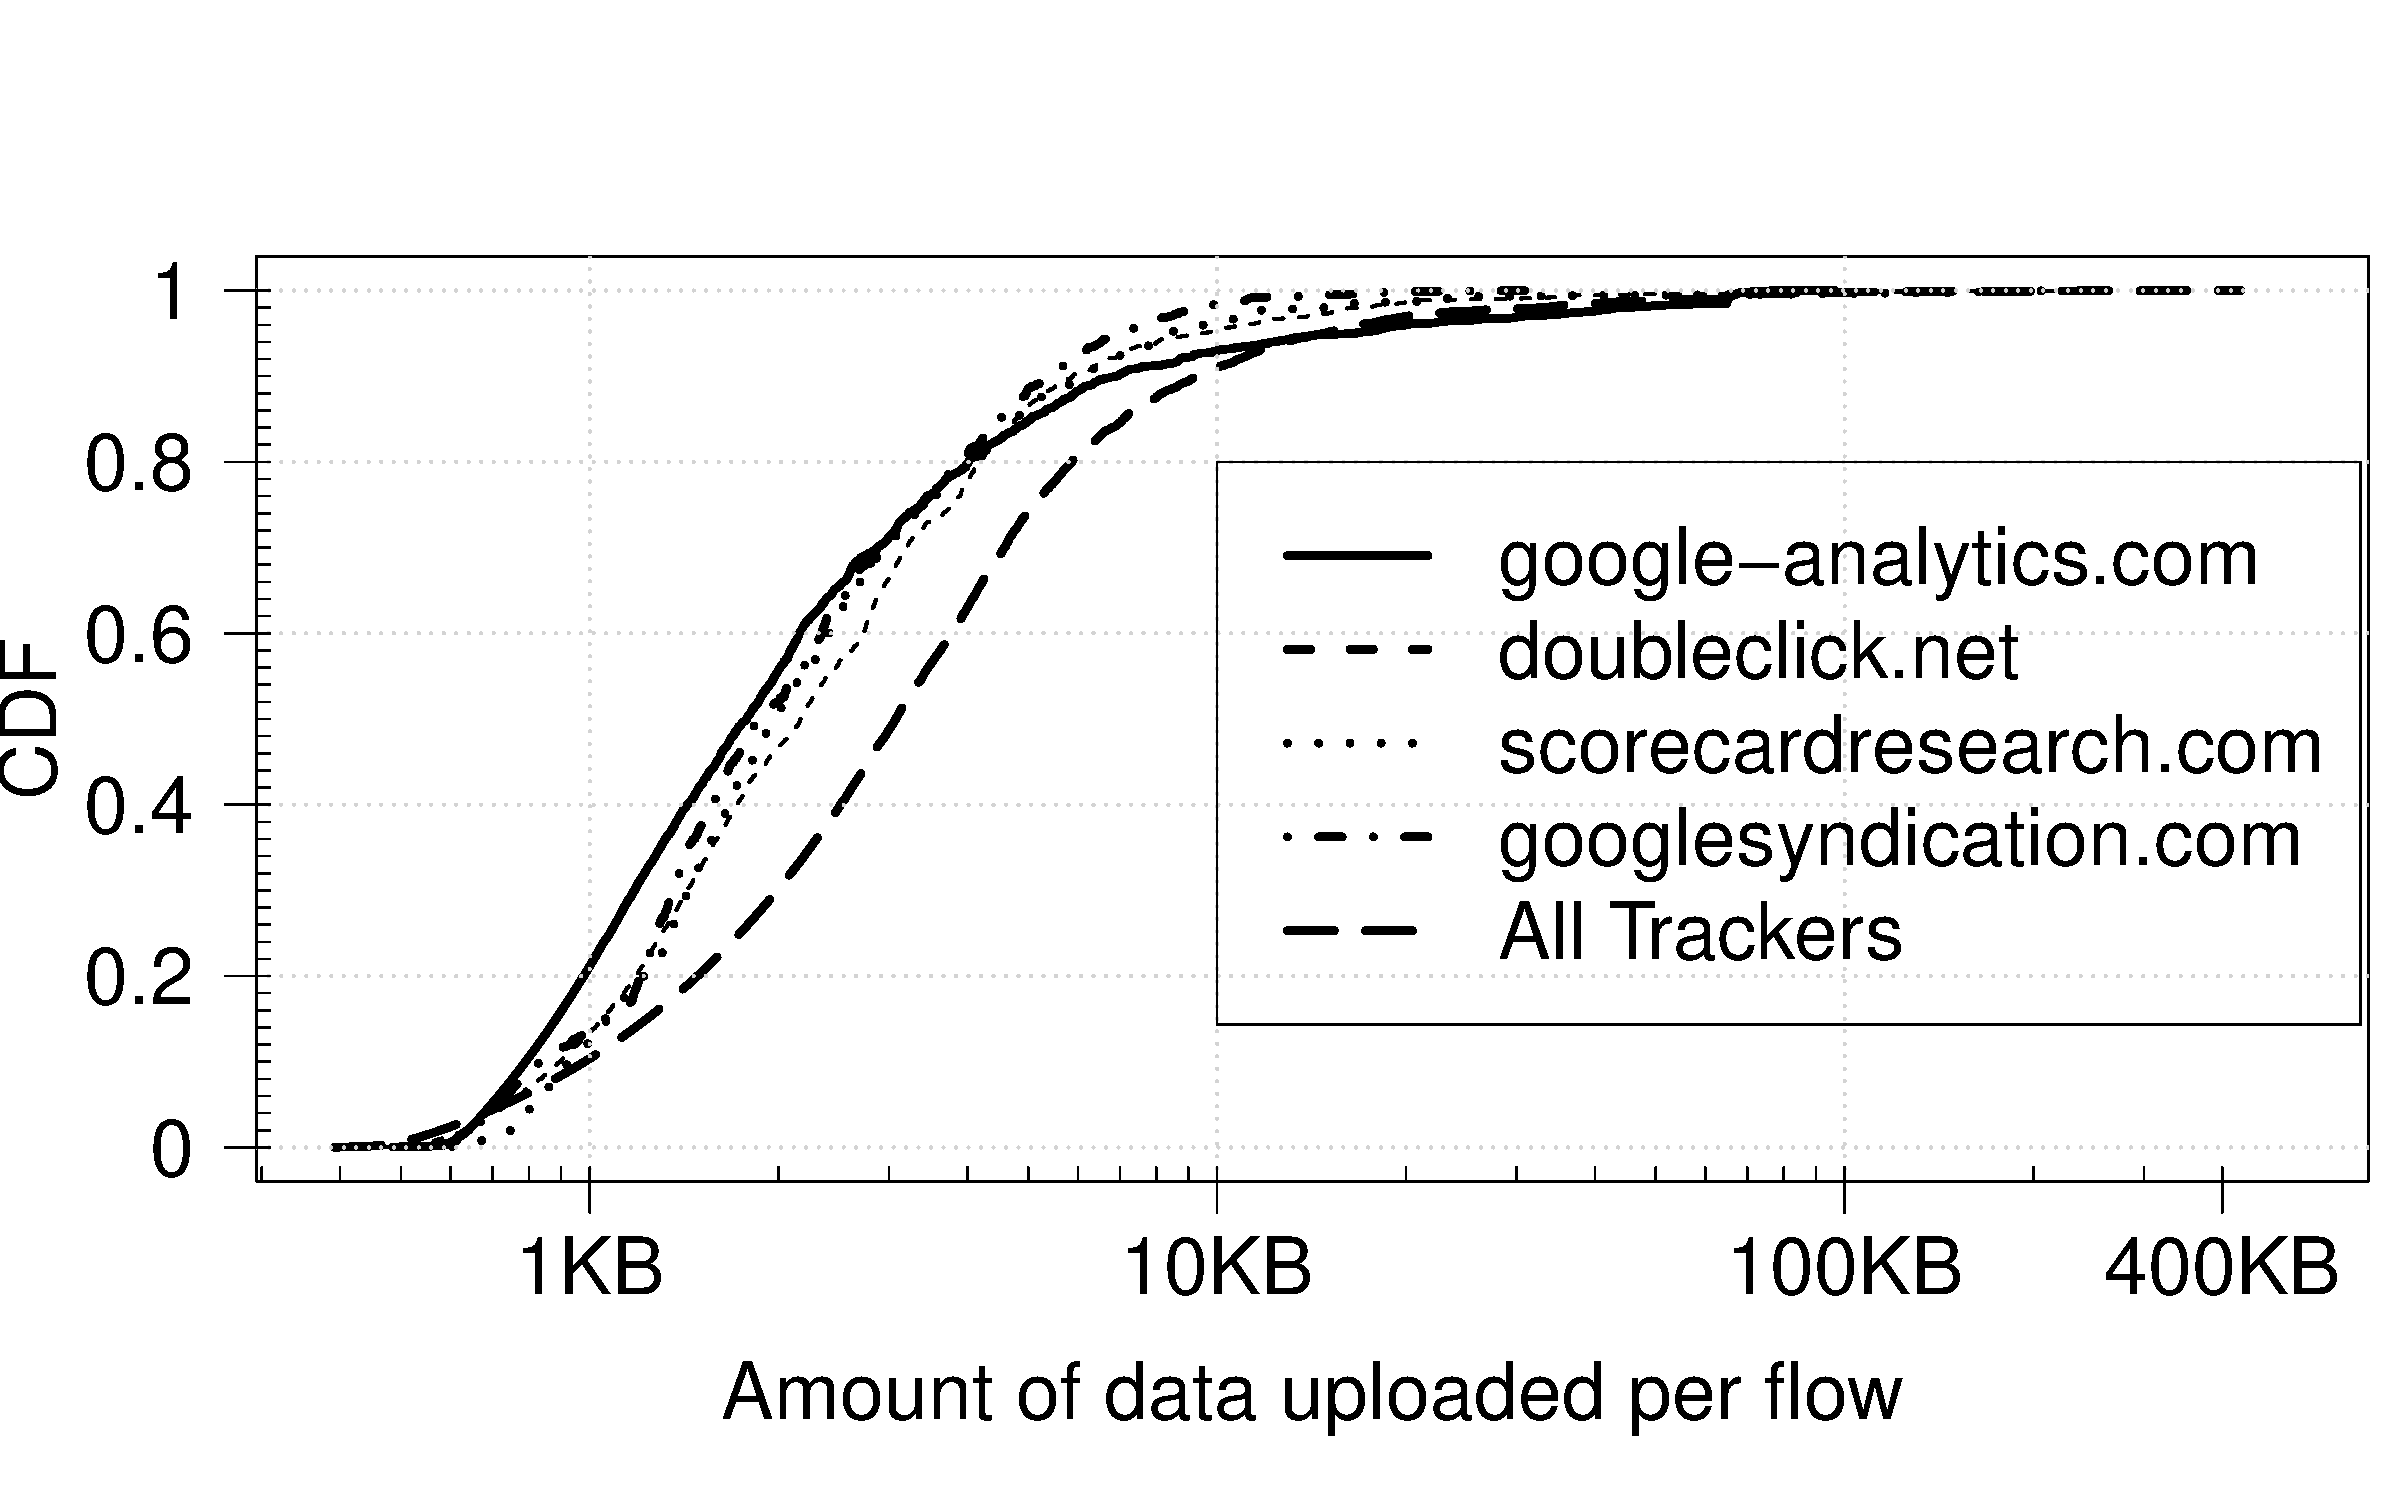
\includegraphics[width=\columnwidth]{plots/distrib_ad_uploads.pdf}
\caption{Distribution of bytes uploaded by ads and analytics sites. \emph{The distribution of bytes uploaded by all ads and analytics sites and the top four ads sites based on traffic volume across all users}.}
\label{fig:description}
\end{figure}

\begin{figure}[t]
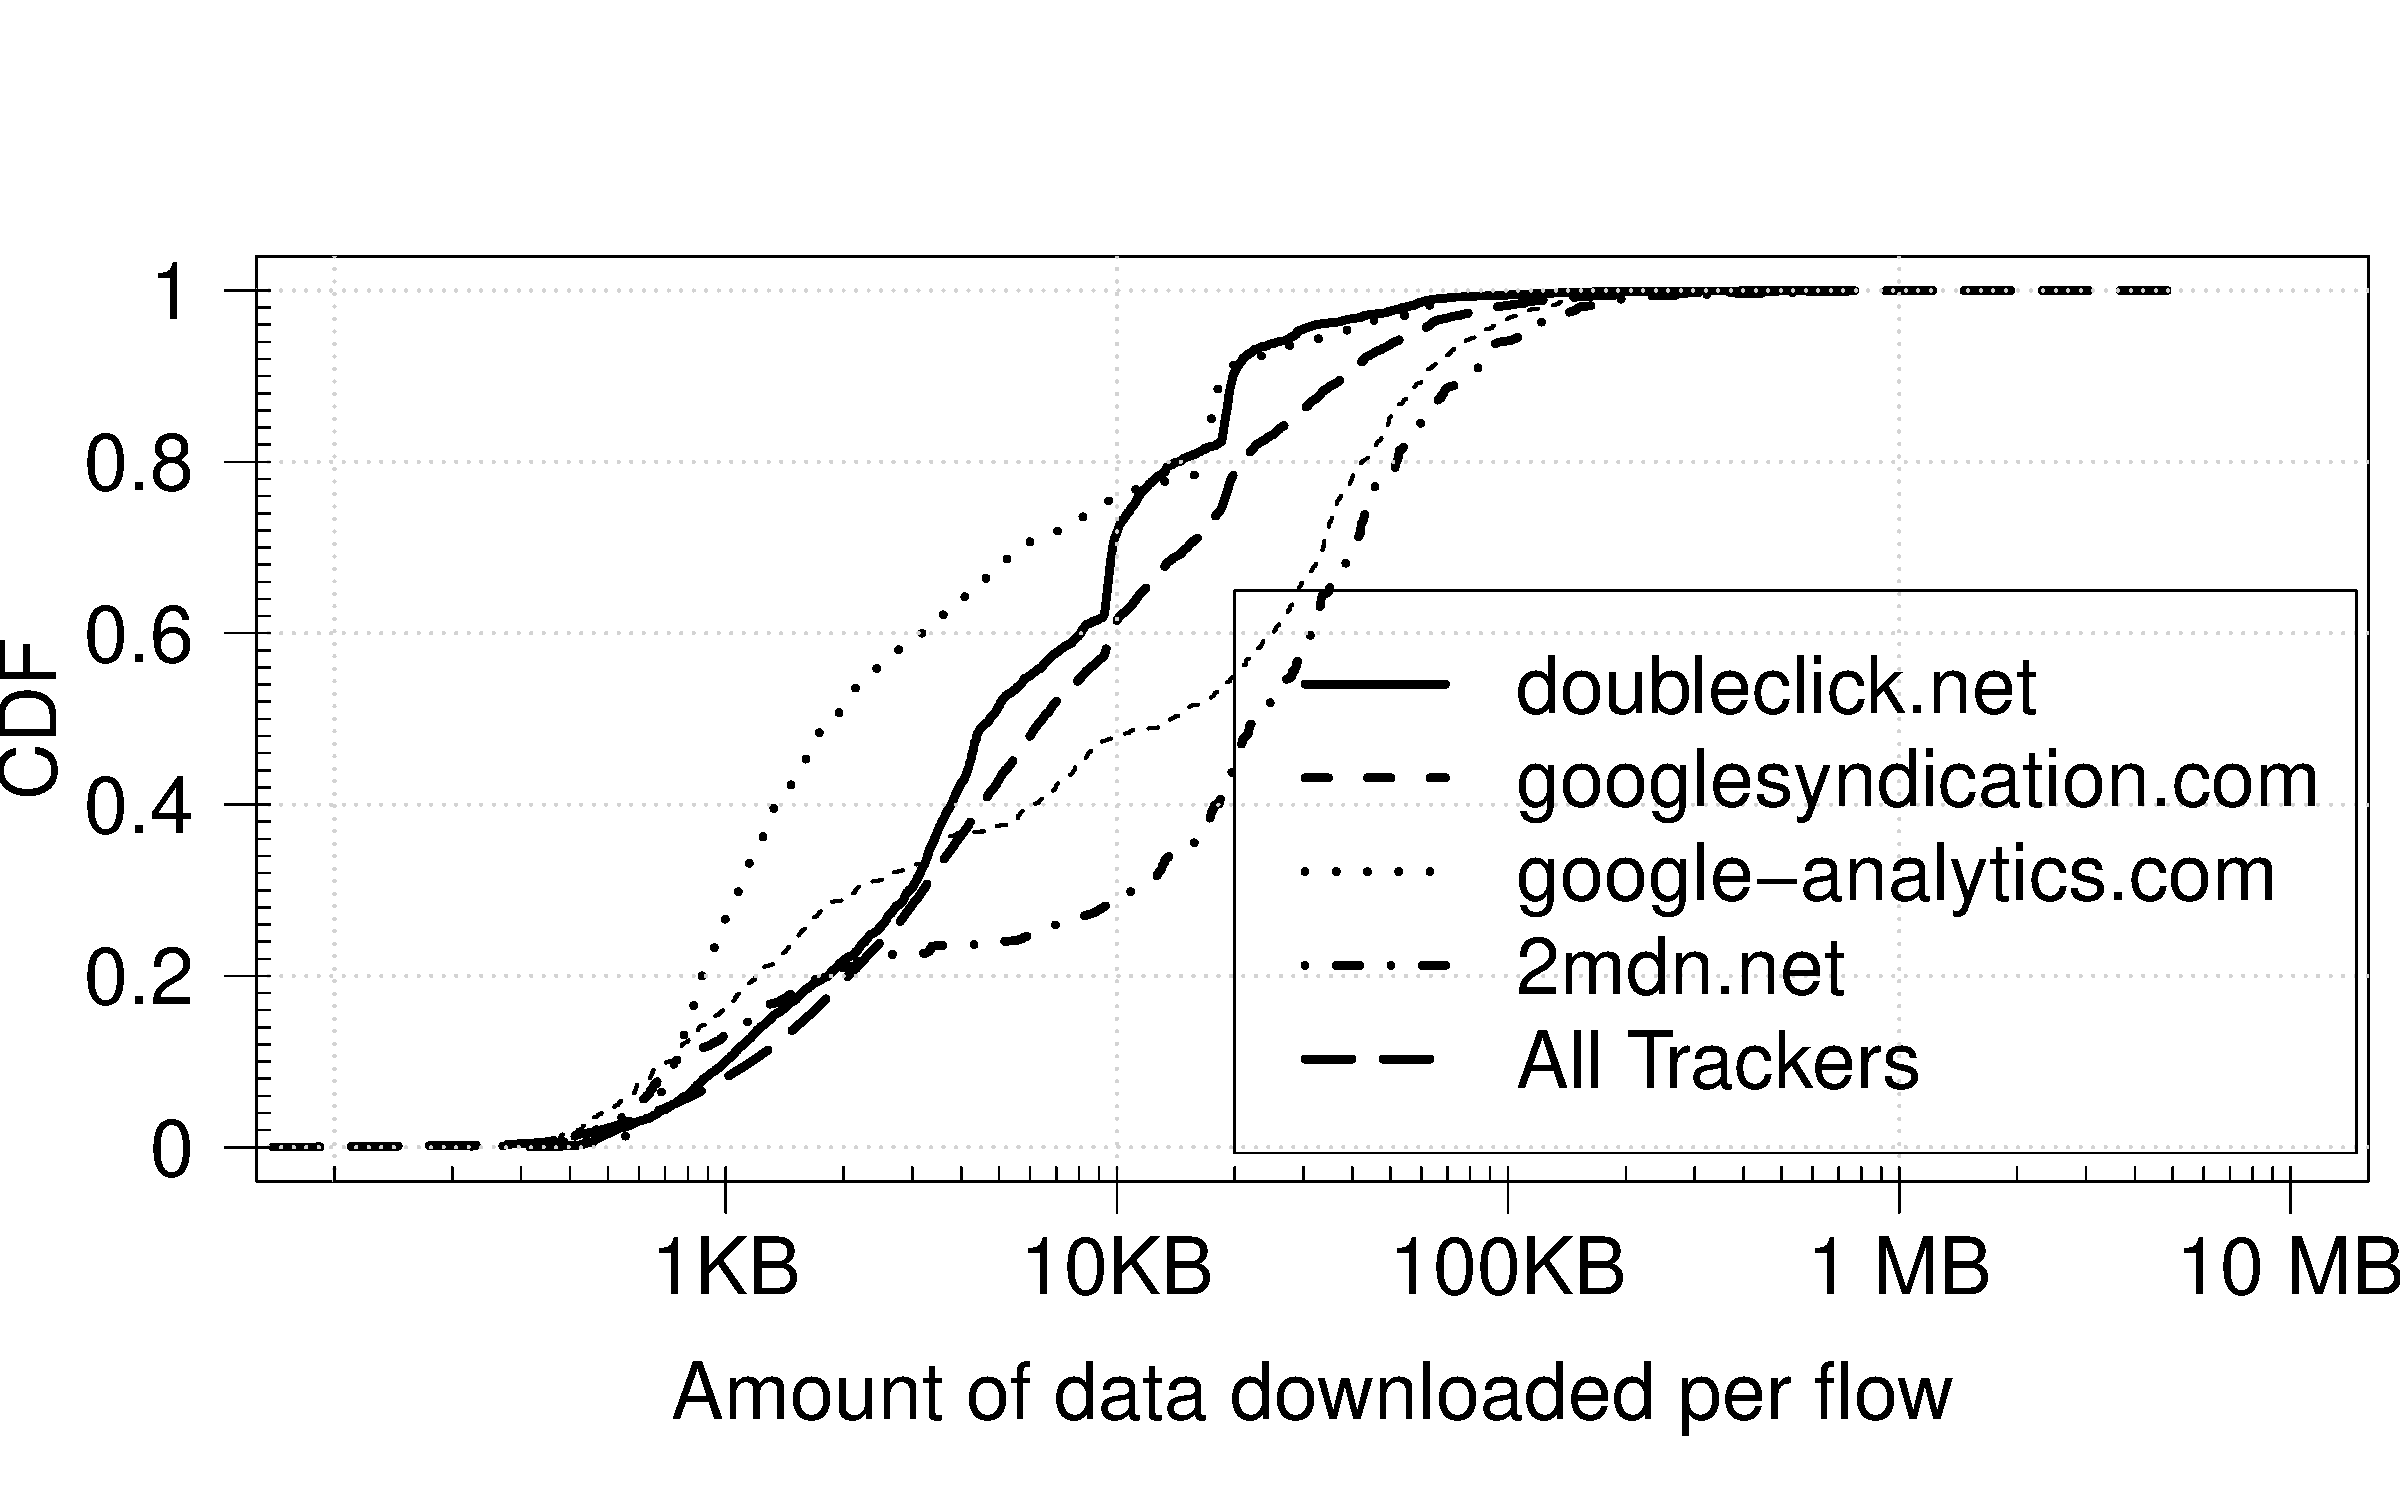
\includegraphics[width=\columnwidth]{plots/distrib_ad_downloads.pdf}
\caption{Distribution of bytes downloaded by ads and analytics sites. \emph{The distribution of bytes uploaded by all ads and analytics sites and the top four ads sites based on traffic volume across all users}.}
\label{fig:description}
\end{figure}

\begin{table}[t]
\centering
\begin{small}
\begin{tabular}{|p{0.35\columnwidth}|p{0.1\columnwidth}|p{0.15\columnwidth}|p{0.1\columnwidth}|}
\hline
\multirow{2}{*}{\bf Tracker} & \multicolumn{3}{c|}{\bf Number of devices tracked}\tabularnewline
\cline{2-4}
   &  {\bf Total} & {\bf Android} & {\bf iOS} \tabularnewline
\hline
doubleclick.net & 25 & 11 & 14 \tabularnewline
\hline
google-analytics.com   & 25 & 11 & 14 \tabularnewline
\hline
googlesyndication.com  & 22 & 10 & 12 \tabularnewline
\hline
admob.com  & 21 & 10 & 11 \tabularnewline
\hline
scorecardresearch.com &  21 & 10 & 11 \tabularnewline
\hline
2mdn.net  &  20 & 9 &  11 \tabularnewline
\hline
atdmt.com  & 18 & 9 &  9 \tabularnewline
\hline
imrworldwide.com & 18 &  9 &  9 \tabularnewline
\hline
flurry.com & 17 & 7 &  10 \tabularnewline
\hline
googleadservices.com  & 17 & 8 &  9 \tabularnewline
\hline
\end{tabular}
\end{small}
\caption{The top 10 ads and analytics sites that tracked the devices in our dataset.
\emph{Two trackers, \emph{doubleclick.net} and\emph{google-analytics.com}, were tracking all the 25 devices in our dataset.}}
\label{tab:top_trackers}
\end{table}


\begin{table*}[t]
    \begin{tabular}{l|l|l|l|l|l|l|l|l|l|l}
       Dataset&Platform&Proto&\# Apps&Email&Location&Username&Password&Android ID&Contacts&IMEI\\
       \hline
       Google Play&Android&HTTP&100&?&10 (10\%)&7 (7\%)&1 (1\%)&21 (21\%)&0 (0\%)&13 (13\%)\\
       \hline
       Third Party&Android&HTTP&908&?&32 (3.5\%)&?&0 (0\%)&95 (10.4\%)&4 (0.4\%)&48 (5.3\%)\\
       \hline
       App Store&iPhone&HTTP&100&?&?&?&?&?&?&?\\
    \end{tabular}
    \caption{\label{tbl:pii}Summary of personally identifiable information leaked in plaintext (HTTP) by Android and iPhone apps.}
  \end{table*}
  

  {\bf Android Apps.}
  When we inspect the data from our controlled study, we see that some apps contact a large number of external servers while others contact significantly fewer.
  In Figure~\ref{fig:android-cdns}, we show both the total number of servers contacted (solid lines) as well as the number of organizations contacted (dotted lines) for both the top-100 Google Play dataset and the top-2000 third-party dataset.
  To quantify ``organizations contacted'', we performed whois lookups on all servers contacted and mapped them to an organization name, allowing us to tighten our upper bound on the number of companies/entities able to track the user through a single app.
  Returning to the figure, we see...~\ref{fig:android-cdns}...\tbd{Amy...}


  {\bf iPhone Apps.}
  \tbd{Shen...}

\subsection{Personally Identifiable Information}
 
  Finally, we turn to information leaked by individual applications. We do not report on data leaked for our real users here, but only the data leaked by our controlled apps in isolation.
  We created fake user accounts on the test phones for a fake user named ``Tess Droid'', with fake contact information and fake Twitter and Facebook accounts. 
  We were then able to check that none of this data ever was released over the network, either in plaintext (HTTP) or encrypted (HTTPS, see \S\ref{sec:bumping}).
  
  We consider data to be `leaked' when any personally identifiable information -- email address, phone number, IMEI number -- is sent across the network under HTTP or HTTPS.
  Some of this information may be relevant to the app -- \eg{}, many apps legitimately require email access. 
  However, none of this information should ever travel across the network in plaintext (HTTP), which we see violated in serveral cases.

  In Table~\ref{tbl:pii}, we see the type of PII leaked for both Android and iPhone apps.
  For Android apps, IMEI and Android ID are the most commonly leaked forms of PII in both the Google Play and third-party dataset.
  Although not popularly thought of as ``private'' data, each of these identifiers are globally unique: IMEI is a unique identifier tied to a phone, and an Android ID is an identifier tied to a user's Google Account, used across many services on the Internet. 
  Consequently, either of these datapoints can be used to track or correlate a user's behavior across all sites the user visits that sell or collaborate with tracking data: a user's behavior on one site can easily be linked to their behavior on any other site they visit.
  With Android ID being tracked by between 10 and 20\% of apps in our study, and IMEI being tracked by between 5\% and 13\% of apps in our study, this suggests that global user tracking across collaborating services can be easily achieved today just by using this identifier.
  \tbd{...}

  Other informaiton like contacts, email, and passwords were rarely leaked in the clear, but all were leaked on occaision, suggesting that stricter monitoring of Android app behavior is needed -- contrastingly, no iPhone apps (which are manually given clearance by Apple before hitting the iPhone store) leaked passwords in plaintext~\tbd{is this true.}

  Moving to iPhone apps, \tbd{...}
%\subsection{Characterize Facebook Applications}

%Why Facebook was chosen?

%What do we observe ?

%What do we see in the User Agent Fields. 



{\footnotesize
\bibliographystyle{abbrv}
\bibliography{biblio}
}
\end{document}
%%% Local Variables: ***
%%% mode:latex ***
%%% TeX-master: "main.tex"  ***
%%% End: ***

